\documentclass[11pt,a4paper]{article}

\usepackage[margin=2.5cm]{geometry}
\usepackage{amsmath,amssymb}
\usepackage{graphicx}
\usepackage{booktabs}
\usepackage{caption}
\usepackage[numbers,sort&compress]{natbib}
\usepackage{xcolor}
\definecolor{linkcol}{RGB}{25,60,130}
\usepackage[colorlinks=true,linkcolor=linkcol,citecolor=linkcol,urlcolor=linkcol]{hyperref}

\captionsetup{font=small,labelfont=bf}
\graphicspath{{figures/}}

% ---------------------------------------------------------------------------
\title{Physics-informed neural networks on the van der Pol oscillator:\\
a measured comparison of the continuous-time and discrete-time formulations}

\author{George William Scriven\thanks{george.w.scriven@gmail.com}\\[2pt]
\normalsize Maastricht University, Maastricht, The Netherlands\\
\normalsize Hasselt University, Hasselt, Belgium\\
\normalsize Nikhef, Amsterdam, The Netherlands}

\date{\today}

\begin{document}
\maketitle

\begin{abstract}
We rebuild the two formulations of physics-informed neural networks (PINNs)
introduced by Raissi, Perdikaris and Karniadakis on the van der Pol
oscillator and measure both against a fixed-step sixth-order Runge--Kutta
reference trusted to $10^{-13}$, at least six orders of magnitude below any
trained network in this study. The continuous-time formulation, transcribed
faithfully, matches or betters the accuracy reported in the original work
on horizons up to one period of the limit cycle ($3.8\times10^{-5}$ to
$6.6\times10^{-4}$ relative $L_2$ error). Beyond one period it fails
structurally: every seed collapses onto a spurious solution of the
differential equation while the training loss converges, so the failure is
silent. Across 733 training runs under the original optimiser protocol, no resource changes where this happens.
Causal weighting of the residuals, the strongest loss-level modification
available, moves the failure from one period out to two at a cost that
grows faster than linearly. A four-fold extension of the optimisation
budget repairs none of the seven runs it was applied to. A 600-run sweep
over 25 architectures finds no size that repairs a failing horizon, and
added depth is actively harmful. Varying the collocation density 64-fold
has no effect on the plain formulation at the failing horizons, and
targeted re-placement of the collocation points changes nothing. What does
order the outcomes is the starting state: at two periods the causally
weighted formulation reaches better than 1\% error for 12.7\% of the
architecture and start combinations tested, with the successes
concentrated on the outer starts, and at four periods for none. A supervised control then locates the failure: the same networks fit four periods from reference data at a few times $10^{-4}$, so the residual objective, not the network or the optimiser, is what fails. I show why: for an autonomous system every trajectory of the flow satisfies the equation exactly, so a candidate that follows the truth and then splices onto another trajectory, the fixed point being the cheapest, has zero residual at every point of a fixed collocation set and a price of order $1/T$ under resampling. Eight variants of the objective trained to demonstrated convergence, ten seeds each at two, four and six periods, bear this out: every fix works at two periods; past two, every variant of the published fixed-point regulariser converges onto a spliced off-loop trajectory with a loss below $10^{-4}$, and only pseudo-time stepping succeeds, in 8 of 10 seeds at four periods and 7 of 10 at six. Its own wall lies between six and ten periods, its failures are late parks, and the loss of every parked run with a sampled transition layer follows the $1/T$ law to within a few percent at every collocation density. The
discrete-time formulation, generalised so that the network input is the
starting state itself, learns a single reusable implicit Runge--Kutta step
of size $\Delta t = 0.8$ from the equations alone. Swept over the number
of stages against the exactly solved scheme, it is scheme-limited at $q=2$
and network-limited from $q=4$, with an endpoint error floor of
$3.6\times10^{-3}$ that a 135-run architecture sweep shows to be an
optimisation floor rather than a capacity one (rank correlation between
training loss and held-out one-step error $+0.974$). Long-horizon quality
is decided by the training seed, is measurable on a validation chain, and
transfers. A simple selection protocol (train ten seeds, chain each to the
target horizon on validation starts, keep the best) yields a single
network of 4 layers and 32 units that carries 108 held-out starting
states through six periods at $2.0\times10^{-3}$ relative $L_2$ error, a
horizon at which even the causally weighted continuous-time formulation
has an error above one, and that stays flat to thirty periods on fresh
starts. Chaining this map beats the source work's single-large-step mode
by a factor of 10 at the largest feasible step. Finally, a matched
data-supervised twin quantifies the accuracy cost of training from the
equations alone: the equation-trained network lands within a factor 2.1
of perfect-label training at zero reference-data cost.
\end{abstract}

\tableofcontents

% ===========================================================================
\section{Introduction}
\label{sec:intro}

A physics-informed neural network (PINN) is a neural network trained to
satisfy a differential equation: the training loss contains the equation
itself, evaluated on the network's own output by automatic differentiation,
in place of (or in addition to) measured data. The canonical statement of
the idea is the work of Raissi, Perdikaris and
Karniadakis~\cite{raissi2019}, referred to throughout this paper as
\emph{the source work}. It contains two distinct constructions:

\begin{enumerate}
  \item a \textbf{continuous-time} formulation, in which the network
  \emph{is} the solution (time goes in, and space too for a partial
  differential equation; the solution value comes out), with the equation
  enforced at sampled points of the domain; and
  \item a \textbf{discrete-time} formulation, in which the network predicts
  the internal stage states of one implicit Runge--Kutta step and the
  algebra of the step itself supplies the supervision.
\end{enumerate}

In this paper I rebuild both constructions from scratch on a single,
completely controlled test problem, the van der Pol
oscillator~\cite{vanderpol1926}, a two-dimensional nonlinear system with an
attracting limit cycle, and measure them under identical optimiser
discipline against a reference solution whose own error is negligible. The
oscillator is small enough to measure exhaustively and hard enough to
defeat naive fits. My wider motivation is the construction of learned
surrogates for ordinary differential equations arising in charged-particle
track reconstruction~\cite{aaij2020}, for which a controlled proving ground
was required. The study asks where each formulation stops working, by what
mechanism, and what the strongest available modification costs, rather
than simply whether it can work. The evidence base is 733 training runs on the continuous-time side under the original protocol, a further 654 in the failure study of Sections~\ref{sec:control} to~\ref{sec:axes} (24 supervised, 150 at a fixed budget, 240 trained to convergence, 240 on density and horizon), and 241 on the discrete-time side.

The contributions are:

\begin{enumerate}
  \item a faithful reproduction of the continuous-time formulation that
  matches the source work's reported accuracy up to one period of the limit
  cycle and fails beyond it by collapsing onto spurious solutions of the
  equation with a converged training loss. The problem is well-posed with a
  unique solution and the collocation budget is trivially affordable, so
  this is a measured counterexample to the source work's stated expectation
  that a sufficiently expressive network with sufficiently many collocation
  points achieves good accuracy on a well-posed problem
  (Sections~\ref{sec:cont-method} and~\ref{sec:cont-results});
  \item a demonstration that the failure is structural, by measuring that
  no resource changes the outcome: a four-fold optimisation budget repairs
  none of the seven runs that ended with the step budget spent
  (Section~\ref{sec:causal}); a 600-run sweep over 25
  architectures and six starting states finds no size that repairs a
  failing horizon, with added depth harmful
  (Section~\ref{sec:size-start}); the collocation density, varied over a
  64-fold range, moves the plain formulation's failing-horizon medians by
  at most a factor 1.15 (Section~\ref{sec:density}); and targeted
  re-placement of the collocation points changes nothing (Section~\ref{sec:placement}), all under the original L-BFGS protocol; with training taken to a demonstrated plateau, density does help at two periods while the four-period wall stays (Section~\ref{sec:axes});
  \item an identification of what does order the outcomes: the starting
  state. Success at two periods occurs in 19 of the 150 causally weighted
  runs (12.7\%) at the 1\% error threshold and depends on where the start
  sits; at four periods none of the 300 runs of either variant succeeds
  (Section~\ref{sec:size-start});
  \item a measurement of causal weighting~\cite{wang2024causal}, the
  strongest loss-level modification in the literature: it moves the
  failure from one period out to two at a cost that grows faster than
  linearly, makes failures detectable in training telemetry, and carries a
  density floor (approximately 20 collocation points per unit time here)
  below which its weight-based completion condition is met on wrong
  solutions (Sections~\ref{sec:causal} and~\ref{sec:density});
  \item a supervised control that locates the failure: the same networks, sample times, optimiser and caps fit four periods from reference data at $3\times10^{-4}$ to $5\times10^{-3}$ in all 24 runs, so the residual objective is what fails (Section~\ref{sec:control});
  \item an account of why, from the objective itself: every trajectory of the flow satisfies the equation exactly, so spliced candidates, of which the fixed point is the cheapest member, have zero residual on a fixed collocation set and a price of order $1/T$ under resampling; the price is then measured, loss $\times T$ constant to within a few percent over 65 parked runs from four to fifteen periods at every density (Sections~\ref{sec:splice} and~\ref{sec:axes});
  \item a comparison of eight objectives, the published fixed-point regulariser in three variants, resampling, causal weighting and pseudo-time stepping, each trained to a demonstrated plateau at two, four and six periods with ten seeds: every fix works at two periods, every regulariser variant converges onto a spliced off-loop trajectory past them, and only pseudo-time stepping, whose mechanism prices the whole family, succeeds at four and six periods; its own wall lies between six and ten periods and collocation density does not move it (Sections~\ref{sec:arms} and~\ref{sec:axes});
  \item a generalisation of the discrete-time formulation in which the
  network input is the starting state itself, yielding a single reusable
  map that advances any state by a fixed time step, trained from the
  equations alone, following the extension of
  Fern\'andez Corral et al.~\cite{fernandez2024}
  (Section~\ref{sec:disc-method});
  \item an attribution of the discrete-time map's error: sweeping the
  number of implicit Runge--Kutta stages against the exactly solved scheme
  shows it scheme-limited at $q=2$ and network-limited from $q=4$ with a
  floor of $3.6\times10^{-3}$ (Section~\ref{sec:disc-results}). A 135-run
  architecture sweep then shows the floor is an optimisation floor rather
  than a capacity one: training loss and held-out one-step error
  rank-correlate at $+0.974$, so networks that fail also fail to train
  (Section~\ref{sec:disc-size});
  \item a finding that long-horizon quality under chaining is decided by
  the training seed rather than the architecture, together with a selection
  protocol that exploits it: chained error on a validation set predicts
  held-out six-period error at rank correlation $+0.98$, and selecting the
  best of ten seeds yields a single network that holds
  $2.0\times10^{-3}$ relative error to six periods and stays flat to
  thirty (Section~\ref{sec:disc-size});
  \item a head-to-head comparison over identical horizons: the selected
  map, chained without retraining, completes six periods at
  $2.0\times10^{-3}$ relative error where the causally weighted
  continuous-time formulation has an error above one, and beats the
  alternative reading of the source work in which one network learns a
  single large step covering the whole horizon by a factor 10 at the
  largest feasible step, which is bounded by nonlinear solvability rather
  than stability (Section~\ref{sec:disc-routes}); and
  \item a measurement of what the physics loss costs in accuracy: against
  a twin trained on perfect reference labels (799 integrator steps per
  training state), the equation-trained network lands within a factor 2.1
  at zero reference-data cost, and the gap is an optimisation gap
  (Section~\ref{sec:baseline}).
\end{enumerate}

The paper is organised as follows. Section~\ref{sec:problem} fixes the
test problem, the reference solution and the error measures, which
everything later is scored against. Section~\ref{sec:cont-method} is the
complete continuous-time route: the faithful reproduction and its failure
mechanism, causal weighting with its budget-extension test, the three studies that measure the remaining resources, and the failure study that locates the cause in the objective and tests the published fixes (Sections~\ref{sec:control} to~\ref{sec:axes}).
Section~\ref{sec:disc-method} is the complete discrete-time route: the
implicit Runge--Kutta background, the reusable one-step map, the error
attribution, the seed and selection analysis, whole trajectories by
chaining against one large step, and the data-trained comparison.
Section~\ref{sec:discussion} relates the measurements to the claims of the
source work and of the causal-weighting literature;
Section~\ref{sec:future} lists the studies I would run next; and
Section~\ref{sec:conclusion} concludes.

% ===========================================================================
\section{Test problem, reference solution, and metrics}
\label{sec:problem}

\subsection{The van der Pol oscillator}

I use the van der Pol oscillator in first-order form, with state
$y = (y_1, y_2)$ (position and velocity) and damping parameter $\mu$ fixed
at 1 throughout:
\begin{equation}
  \frac{dy_1}{dt} = y_2, \qquad
  \frac{dy_2}{dt} = \mu\,(1 - y_1^2)\,y_2 - y_1 .
  \label{eq:vdp}
\end{equation}
Reading the second equation term by term: for $|y_1| < 1$ the
``damping'' term $\mu(1 - y_1^2)\,y_2$ has the same sign as the velocity
and pumps energy in; for $|y_1| > 1$ it opposes the velocity and takes
energy out. The result is the system's defining feature, a limit cycle:
a closed loop in the $(y_1, y_2)$
plane onto which every trajectory except the equilibrium at the origin
spirals, and around which it then circulates. One period is
$6.663287$ time units, and the loop's extent is $|y_1| \le 2.009$,
$|y_2| \le 2.678$ (both measured from the reference solution below; the
period agrees with the accepted value). The equilibrium at the origin is
repelling: the Jacobian of $f$ there has eigenvalues
$0.5 \pm 0.866\,i$, whose positive real part means nearby solutions grow
like $e^{0.5t}$ while rotating, spiralling outward. Yet the origin
satisfies Eq.~\eqref{eq:vdp} exactly. Both facts drive the failure analysis
of Section~\ref{sec:cont-results}. ``Solving'' the problem means producing
the trajectory from a given starting state over a horizon $T$; the
canonical start throughout is $(2, 0)$, a point on the loop
(Figure~\ref{fig:problem}).

\begin{figure}[tbp]
  \centering
  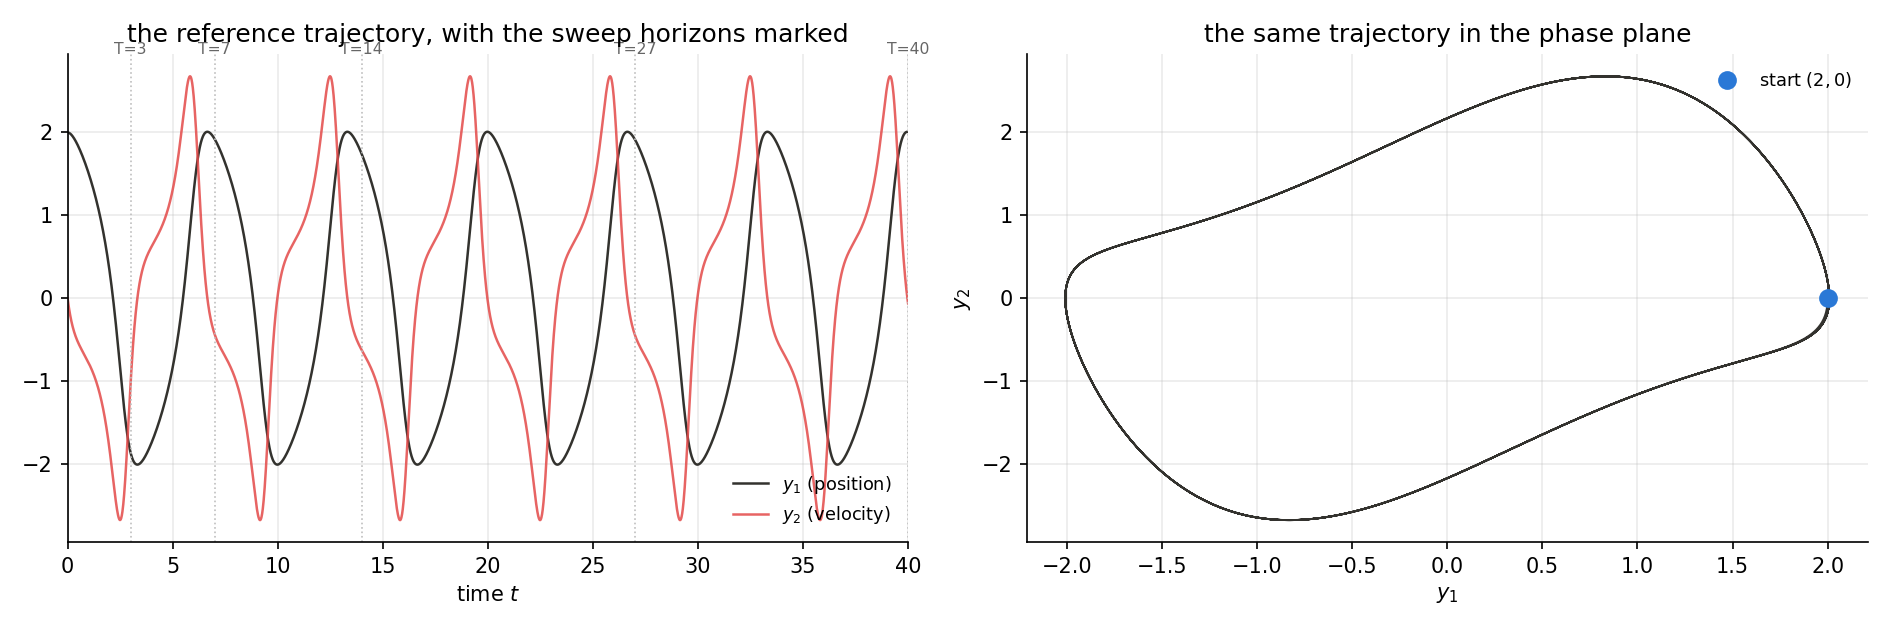
\includegraphics[width=\linewidth]{fig_problem.png}
  \caption{The test problem. Left: the reference trajectory from $(2,0)$
  over six periods, with the five training horizons of the continuous-time
  experiments marked. Right: the same trajectory in the phase plane, the
  closed loop to be learned.}
  \label{fig:problem}
\end{figure}

\subsection{The reference solution}

All errors are measured against a fixed-step, seven-stage, sixth-order
explicit Runge--Kutta integration of Eq.~\eqref{eq:vdp} at step
$10^{-3}$ in double precision, verified independently of any network by
four instruments, each measured rather than asserted:
\begin{enumerate}
  \item the convergence order, measured as the slope of the global error
  against the step size on logarithmic axes over three problems with known
  closed-form solutions (an order-$p$ method appears as slope $p$); the
  measured slopes are 6.06, 6.27 and 5.75 against the theoretical 6;
  \item step-halving self-consistency: integrating at $h$ and $h/2$ and
  comparing, the disagreement reaches a rounding floor of
  $6.4\times10^{-14}$ below $h \approx 5\times10^{-3}$, so at the working
  step $10^{-3}$ the truncation error is beneath double-precision
  rounding;
  \item the period of the limit cycle, $6.663287$ measured against the
  accepted value $6.6633$; and
  \item the closure of the limit cycle onto itself after one full period:
  $5.6\times10^{-14}$.
\end{enumerate}
The reference is trustworthy to approximately $10^{-13}$, at least six
orders of magnitude below anything a trained network reaches in this
study, so the yardstick never contaminates the measurement. The reference
is used only for scoring, never for training, with one deliberate
exception: the data-trained comparison of Section~\ref{sec:baseline},
whose entire point is to consume it. Where a network's evaluation times
fall between stored reference samples (times inside a single step, needed
in Section~\ref{sec:disc-method}), the reference integrator is re-run to
stop exactly at each required time; nothing is interpolated.

\subsection{Error measures}
\label{sec:metrics}

I use three measures. Throughout the paper, whiskered quantities are
medians over random-initialisation seeds with whiskers spanning the
minimum to the maximum seed.
\begin{enumerate}
  \item \textbf{Relative $L_2$ error} (the primary measure):
  $\varepsilon_{\mathrm{rel}} =
  \lVert y_\theta - y_{\mathrm{ref}} \rVert_2 /
  \lVert y_{\mathrm{ref}} \rVert_2$,
  with the norms taken over all evaluation times (or held-out states) and
  both components together; $y_\theta$ denotes the network output and
  $y_{\mathrm{ref}}$ the reference. Explicitly, for a trajectory sampled
  at times $\{t_k\}$,
  $\varepsilon_{\mathrm{rel}}^2 =
  \sum_k \lVert y_\theta(t_k) - y_{\mathrm{ref}}(t_k)\rVert^2 \big/
  \sum_k \lVert y_{\mathrm{ref}}(t_k)\rVert^2$.
  Read it as a fraction of the trajectory's overall size: $10^{-3}$ means
  the prediction differs from the truth by about a tenth of a percent of
  that size, and a value near 1 means the prediction is as wrong as the
  trajectory is large.
  \item \textbf{Scale-normalised pointwise error}:
  $|\hat y_i - y_i| / \max_t |y_{i,\mathrm{ref}}|$ per component, well
  defined even where a component crosses zero; used for error maps and
  curves.
  \item \textbf{Capped pointwise relative error}: the squared error
  normalised by the squared size of the true state and capped at one,
  \begin{equation}
    \rho \;=\; \min\!\left(1,\;
      \frac{\lVert y_{\mathrm{ref}} - y_\theta \rVert^2}
           {\lVert y_{\mathrm{ref}} \rVert^2}\right),
    \qquad
    \lVert y_{\mathrm{ref}} \rVert = \sqrt{y_{1,\mathrm{ref}}^2 + y_{2,\mathrm{ref}}^2},
    \label{eq:rho}
  \end{equation}
  evaluated per point (a time on a trajectory, or a held-out state). A
  worked example fixes the reading: for truth $(2, 0)$ and prediction
  $(1.9, 0.1)$ the error vector is $(0.1, -0.1)$, so
  $\rho = (0.1^2 + 0.1^2)/(2^2 + 0^2) = 0.02/4 = 0.005$; the prediction
  is wrong by half a percent of the state's squared size. ``Capped''
  means the ratio is cut off at one: wherever the squared miss exceeds
  the squared size of the true state, the recorded value is exactly 1,
  read as one hundred percent wrong. The cap exists because the
  denominator can approach zero: near-zero true states would otherwise
  dominate every average, and a miss larger than the state itself carries
  no more information than ``completely wrong''. The
  state-modulus denominator is also deliberate: a
  componentwise denominator is undefined whenever that component crosses
  zero (twice per period for each component, and exactly at the start,
  where $y_2 = 0$), whereas the state modulus vanishes only at the
  equilibrium. In practice the cap engages only on order-one failed fits
  and at evaluation states whose true image is at or near the origin.
  Two reporting rules follow. The \emph{median} of $\rho$ is robust and
  tracks fine structure; the \emph{mean} of $\rho$ (a mean squared
  error, since $\rho$ is already a squared quantity) is dominated by
  capped points, each of which contributes $1/N$ to the mean over an
  $N$-point set, so the mean cannot resolve anything below that level
  and is quoted only together with the number of capped points. Because
  $\rho$ is squared, $\sqrt{\rho}$ compares directly with relative $L_2$
  values, and the two measures cross-check each other throughout (for
  example, the selected network of Section~\ref{sec:disc-size} has
  six-period $\rho = 2.0\times10^{-6}$, i.e.\
  $\sqrt{\rho} \approx 1.4\times10^{-3}$, consistent with its
  independently computed chained relative $L_2$ of $2.0\times10^{-3}$).
\end{enumerate}

% ===========================================================================
\section{The continuous-time formulation}
\label{sec:cont-method}

\subsection{Method}

The source work considers equations $u_t + \mathcal{N}[u] = 0$ and defines
the residual $ r = u_t + \mathcal{N}[u]$ (written $f$ in the source work; this
paper keeps $f$ for the right-hand side of an ordinary differential
equation and writes the residual as $r$). It approximates $u$ by a
network and obtains the residual of the network by automatic
differentiation, the exact, chain-rule differentiation of the network
with respect to its own inputs. The loss is the equally weighted sum of
two mean-squared terms: a data term over the $N_u$ points where the
solution is known (initial and boundary data), and a residual term over
$N_f$ sampled \emph{collocation points},
collocation points being the classical term for locations at which an
equation is enforced.

For an ordinary differential equation the transfer is direct, with three
simplifications and one modification. There is no spatial coordinate:
the network maps one input, time, to the two-component state
$y_\theta(t)$. There is no boundary: the data term collapses to a single
anchor, the requirement that the network at $t = 0$ equal the starting
state. This is one anchored point in place of the 50--100 used by the
source work's demonstrations, which makes the anchor's task
correspondingly harder. No spatial derivatives exist either: the only
differentiation left is the time derivative of the network,
$\dot y_\theta(t)$, obtained by differentiating the network's output with
respect to its own input. Automatic differentiation therefore appears in
two distinct roles that should not be conflated: derivatives of the loss
with respect to the weights $\theta$ drive the optimiser, as in any
network training, while derivatives of the network output with respect to
its input $t$ build the residual itself. Both are exact chain-rule
computations, with no finite differences anywhere. The residual and loss
are the exact transcription of the source construction,
\begin{equation}
  r(t) = \begin{pmatrix}
    \dot y_{1,\theta}(t) - y_{2,\theta}(t) \\[2pt]
    \dot y_{2,\theta}(t) - \mu\big(1 - y_{1,\theta}^2(t)\big)\,
      y_{2,\theta}(t) + y_{1,\theta}(t)
  \end{pmatrix},
  \qquad
  \mathcal{L} = \big\lVert y_\theta(0) - y^0 \big\rVert^2
  + \frac{1}{N}\sum_{i=1}^{N} \big\lVert r(t_i) \big\rVert^2 ,
  \label{eq:contloss}
\end{equation}
with $y^0 = (2,0)$ and $\{t_i\}$ the collocation times. The one deviation:
time is mapped to $[-1,1]$ inside the network, because
hyperbolic-tangent layers condition badly on raw inputs of size 40. The formulation also inherits a structural
limitation from the source work: the starting state enters through the loss
and is baked into the trained weights, so each trained network serves
exactly one initial condition.\footnote{An expensive way to solve one
initial-value problem, and an equally expensive way to solve each
subsequent one.} The discrete-time formulation of
Section~\ref{sec:disc-method} removes exactly this.

\subsection{Collocation budget}
\label{sec:collocation}

Because the collocation budget is central to how the source work frames the
limitations of this formulation, I fix it explicitly and generously. The
density is 20 collocation points per unit time at every horizon, placed by
one-dimensional Latin hypercube sampling (a stratified random design: one
point per equal-width stratum, so the domain is covered without
clustering). A longer horizon therefore receives proportionally more
points and is never undersampled by construction:
$N = 60,\ 140,\ 280,\ 540,\ 800$ collocation points at the five horizons of
Table~\ref{tab:expA}. For comparison, the source work's continuous-time
demonstrations use $20{,}000$ collocation points (Schr\"odinger equation)
and $10{,}000$ (Burgers equation) over two-dimensional space--time domains.
On this problem the entire budget costs fractions of a second to evaluate;
every experiment below pays it in full. Whatever fails in
Section~\ref{sec:cont-results} therefore does not fail for want of
collocation points. Sections~\ref{sec:density} and~\ref{sec:placement}
then vary the density over a 64-fold range and the placement directly,
and measure the effect of each.

\subsection{Protocol}
\label{sec:cont-protocol}

All continuous-time experiments share: a fully connected network of 4
hidden layers of 50 hyperbolic-tangent units, in double precision (until
Section~\ref{sec:size-start} varies the architecture). Written out, the
network computes
\begin{equation*}
  h_1 = \tanh(W_1 t + b_1), \quad
  h_k = \tanh(W_k h_{k-1} + b_k) \;\; (k = 2, \dots, 4), \quad
  y_\theta(t) = W_5 h_4 + b_5 ,
\end{equation*}
with the weight matrices and bias vectors $W_k, b_k$ collectively
denoted $\theta$. The hyperbolic tangent is used because it is smooth
everywhere, and smoothness matters here: the residual of
Eq.~\eqref{eq:contloss} differentiates the network, so a kinked
activation such as the rectifier would hand the residual a discontinuous
derivative. Training horizons are
$T \in \{3, 7, 14, 27, 40\}$, i.e.\ 0.45 to 6.0 periods of the limit
cycle (dividing by the period $6.663287$), bracketing one period from
either side, with three
random-initialisation seeds per horizon, so that a single initialisation
cannot masquerade as the method's verdict.\footnote{A seed fixes the
random initial weights and nothing else; a run is otherwise deterministic,
so every number in this paper reproduces bit for bit.} The optimiser is
full-batch L-BFGS (a deterministic quasi-Newton method using the entire
loss at every step, as in the source work) with strong Wolfe line search.
Every iteration uses the full set of collocation points, so one iteration
is one epoch. Training runs in restarts of 200 epochs, where a restart
clears the optimiser's stored curvature history and continues from the
current weights; there are at most 6 restarts, so at most $1{,}200$
epochs, and training stops early once two consecutive restarts improve
the loss by less than 1\%. This is a convergence criterion rather than a
budget, and every plain-formulation failure below is a converged failure.
Scoring is on the dense reference grid (spacing $0.01$) with the measures
of Section~\ref{sec:metrics}.

\subsection{Results: faithful reproduction}
\label{sec:cont-results}

\begin{table}[tbp]
  \centering
  \caption{Faithful reproduction of the continuous-time formulation, swept
  over the training horizon. $N$ is the number of collocation points
  (density fixed at 20 per unit time). Median, best and worst are over
  three seeds; the loss is the converged training loss.}
  \label{tab:expA}
  \small
  \begin{tabular}{cccccc}
    \toprule
    $T$ & periods & $N$ & rel.\ $L_2$ (median) & best / worst seed & final loss \\
    \midrule
    3  & 0.45 & 60  & $3.8\times10^{-5}$ & $2.3\times10^{-5}$ / $4.6\times10^{-5}$ & $1.4$--$2.0\times10^{-7}$ \\
    7  & 1.05 & 140 & $6.6\times10^{-4}$ & $4.8\times10^{-4}$ / $3.9\times10^{-3}$ & $2.3\times10^{-6}$--$2.8\times10^{-5}$ \\
    14 & 2.10 & 280 & $0.79$             & $0.789$ / $0.805$                       & $\approx 6\times10^{-2}$ \\
    27 & 4.05 & 540 & $0.90$             & $0.903$ / $0.905$                       & $\approx 3\times10^{-2}$ \\
    40 & 6.00 & 800 & $0.94$             & $0.936$ / $2.09$                        & $2.1$--$4.8\times10^{-2}$ \\
    \bottomrule
  \end{tabular}
\end{table}

Table~\ref{tab:expA} and Figure~\ref{fig:cliff} give the central result of
the reproduction. Below one period the formulation is excellent: at
$T = 3$ the median relative $L_2$ error is $3.8\times10^{-5}$, at or better
than the accuracy the source work reports for its own continuous-time
demonstrations ($1.97\times10^{-3}$ for the Schr\"odinger equation,
$6.7\times10^{-4}$ for the Burgers equation). This is unsurprising for a
two-state oscillator against partial differential equations, but it
confirms that the machinery is correctly built. Beyond one period the
error is of order one at every horizon and every seed, with the seeds
agreeing to two decimal places: the failure is systematic, not
initialisation dependent.

\begin{figure}[tbp]
  \centering
  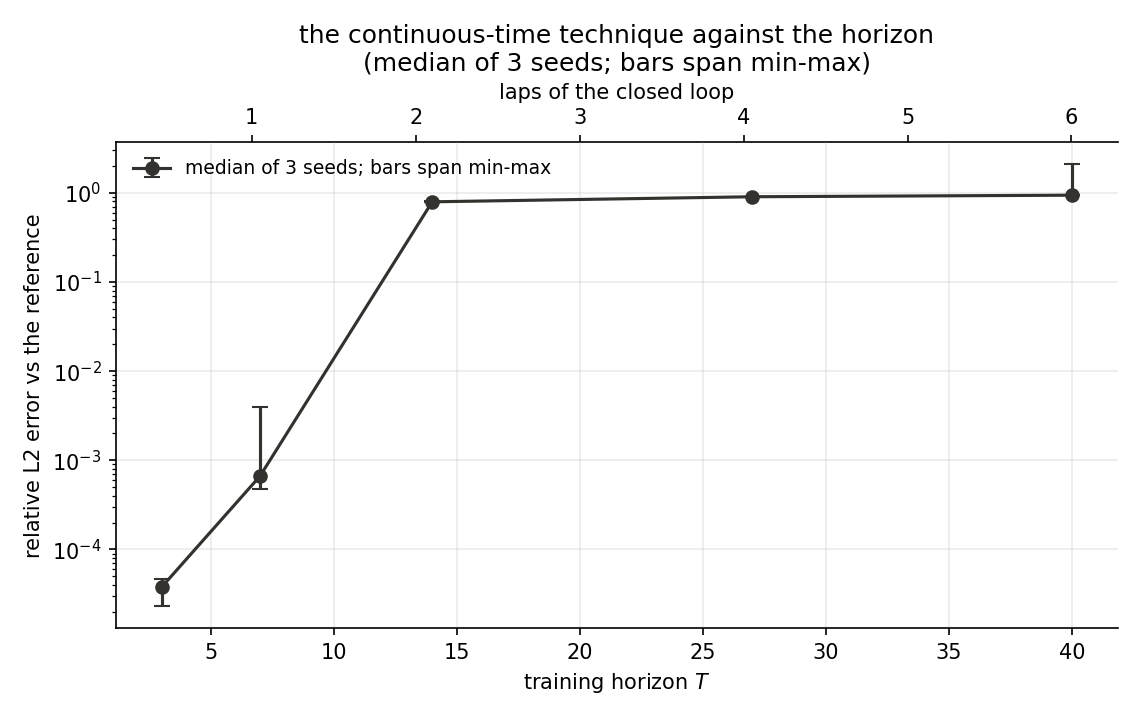
\includegraphics[width=0.72\linewidth]{fig_cliff.png}
  \caption{Relative $L_2$ error against training horizon for the faithful
  reproduction; median of three seeds with min--max whiskers. The
  formulation is excellent below one period of the limit cycle and its
  error is of order one beyond it.}
  \label{fig:cliff}
\end{figure}

\begin{figure}[tbp]
  \centering
  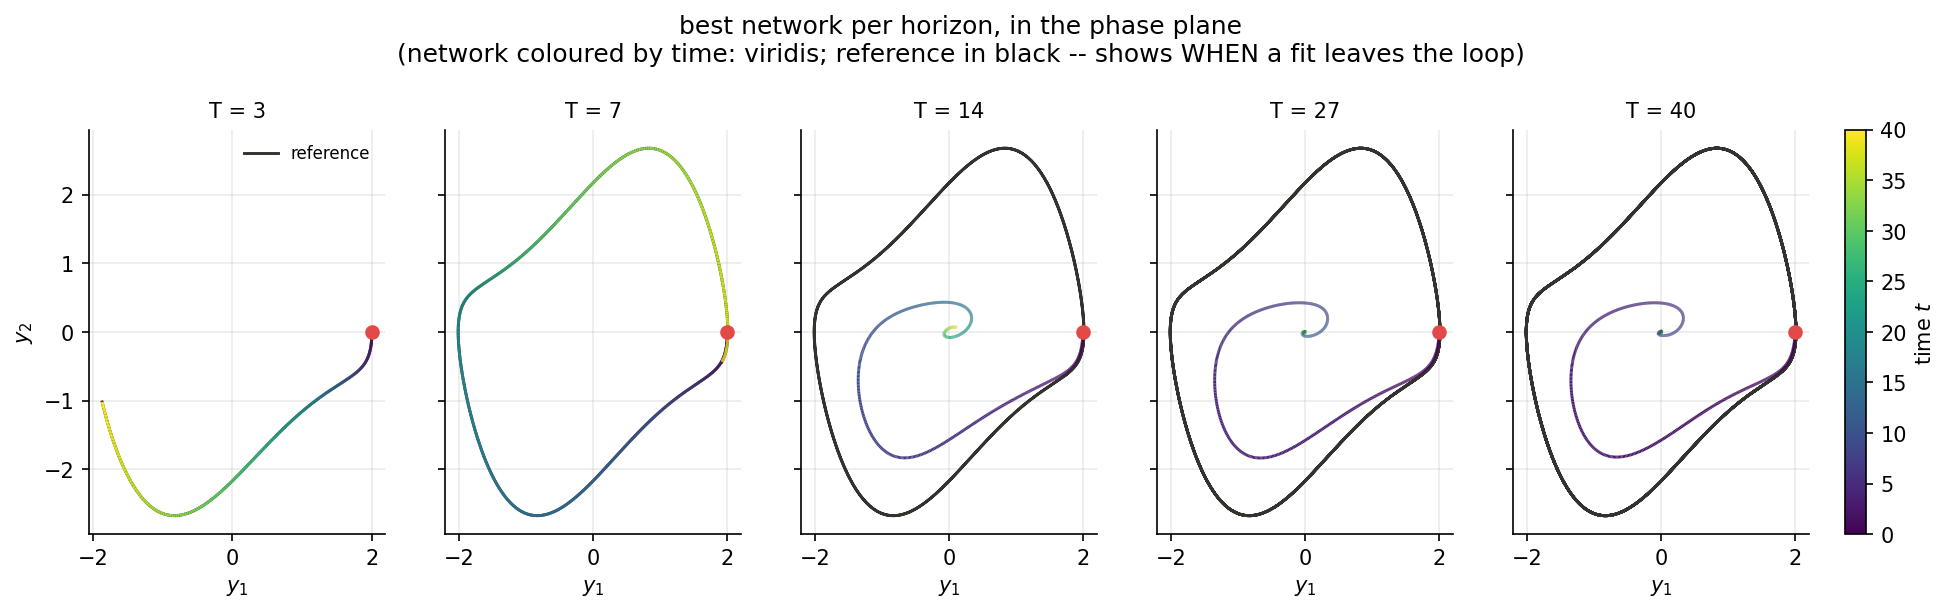
\includegraphics[width=\linewidth]{fig_phase_collapse.png}
  \caption{The failed fits in the phase plane (best seed per horizon).
  Past one period the fit abandons the closed loop and spirals
  into the origin, the repelling equilibrium, against the direction of the
  true flow.}
  \label{fig:phase-collapse}
\end{figure}

\begin{figure}[tbp]
  \centering
  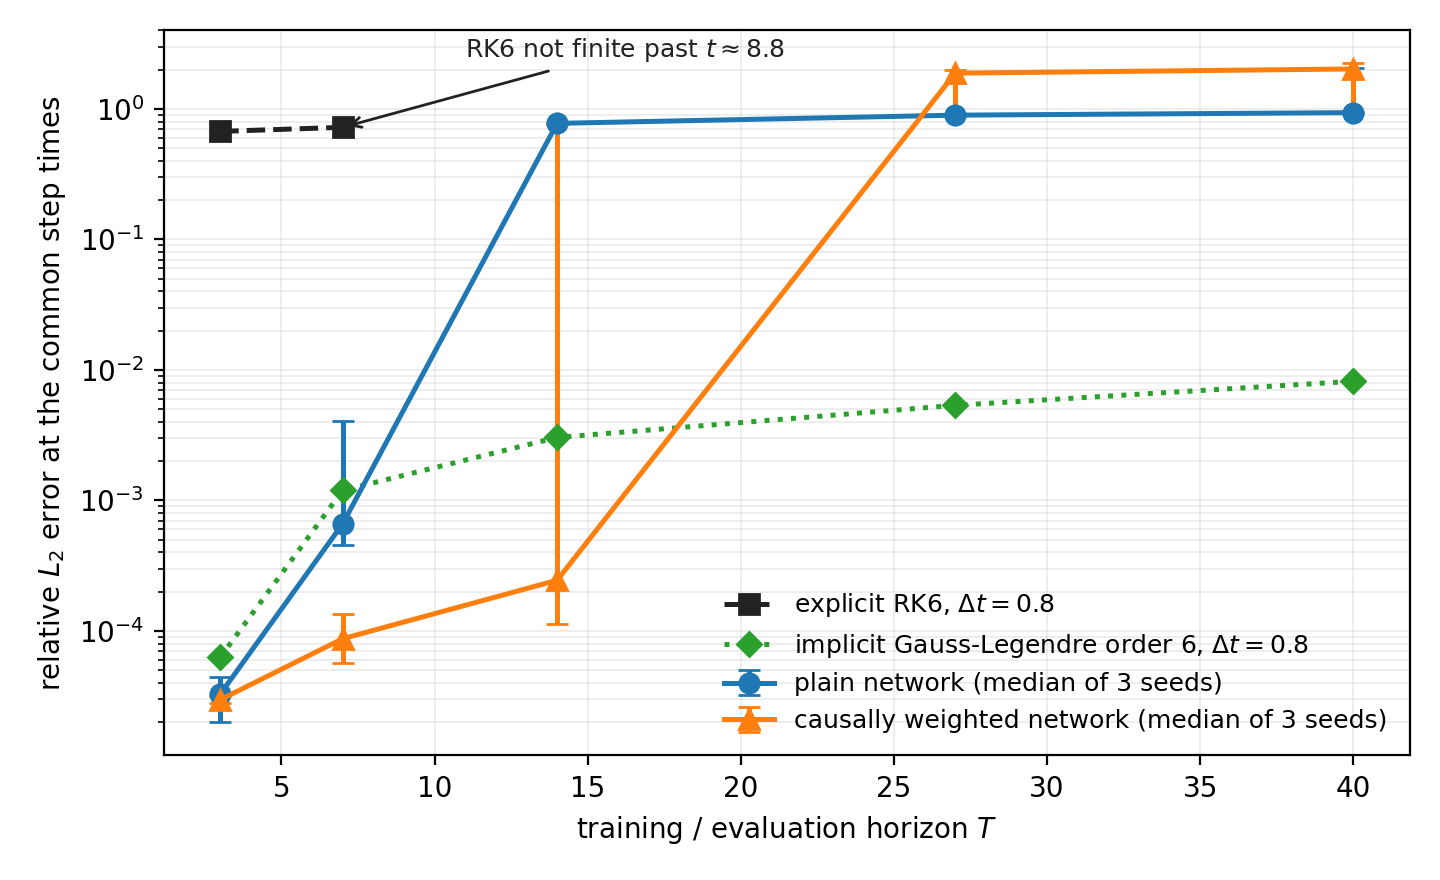
\includegraphics[width=0.85\linewidth]{fig_rk6_comparison.png}
  \caption{A classical anchor for the comparison: the two order-6
  methods at the discrete-time study's step $\Delta t = 0.8$ from the
  same start, against the plain and causally weighted networks. The
  explicit method is the reference integrator's own seven-stage tableau;
  the implicit one is Gauss--Legendre with $q = 3$ (also order 6),
  solved by root-finding. All four are scored identically: relative
  $L_2$ against the reference over the common step times
  $\{0, 0.8, 1.6, \dots\} \le T$ (network medians over three seeds with
  min--max whiskers; the classical runs are deterministic). The explicit
  method at this step is order-one wrong from the first horizon and its
  state is not finite past $t = 8.8$, so it has no value at $T \ge 14$;
  the implicit method is stable at every horizon.}
  \label{fig:rk6}
\end{figure}

\begin{figure}[tbp]
  \centering
  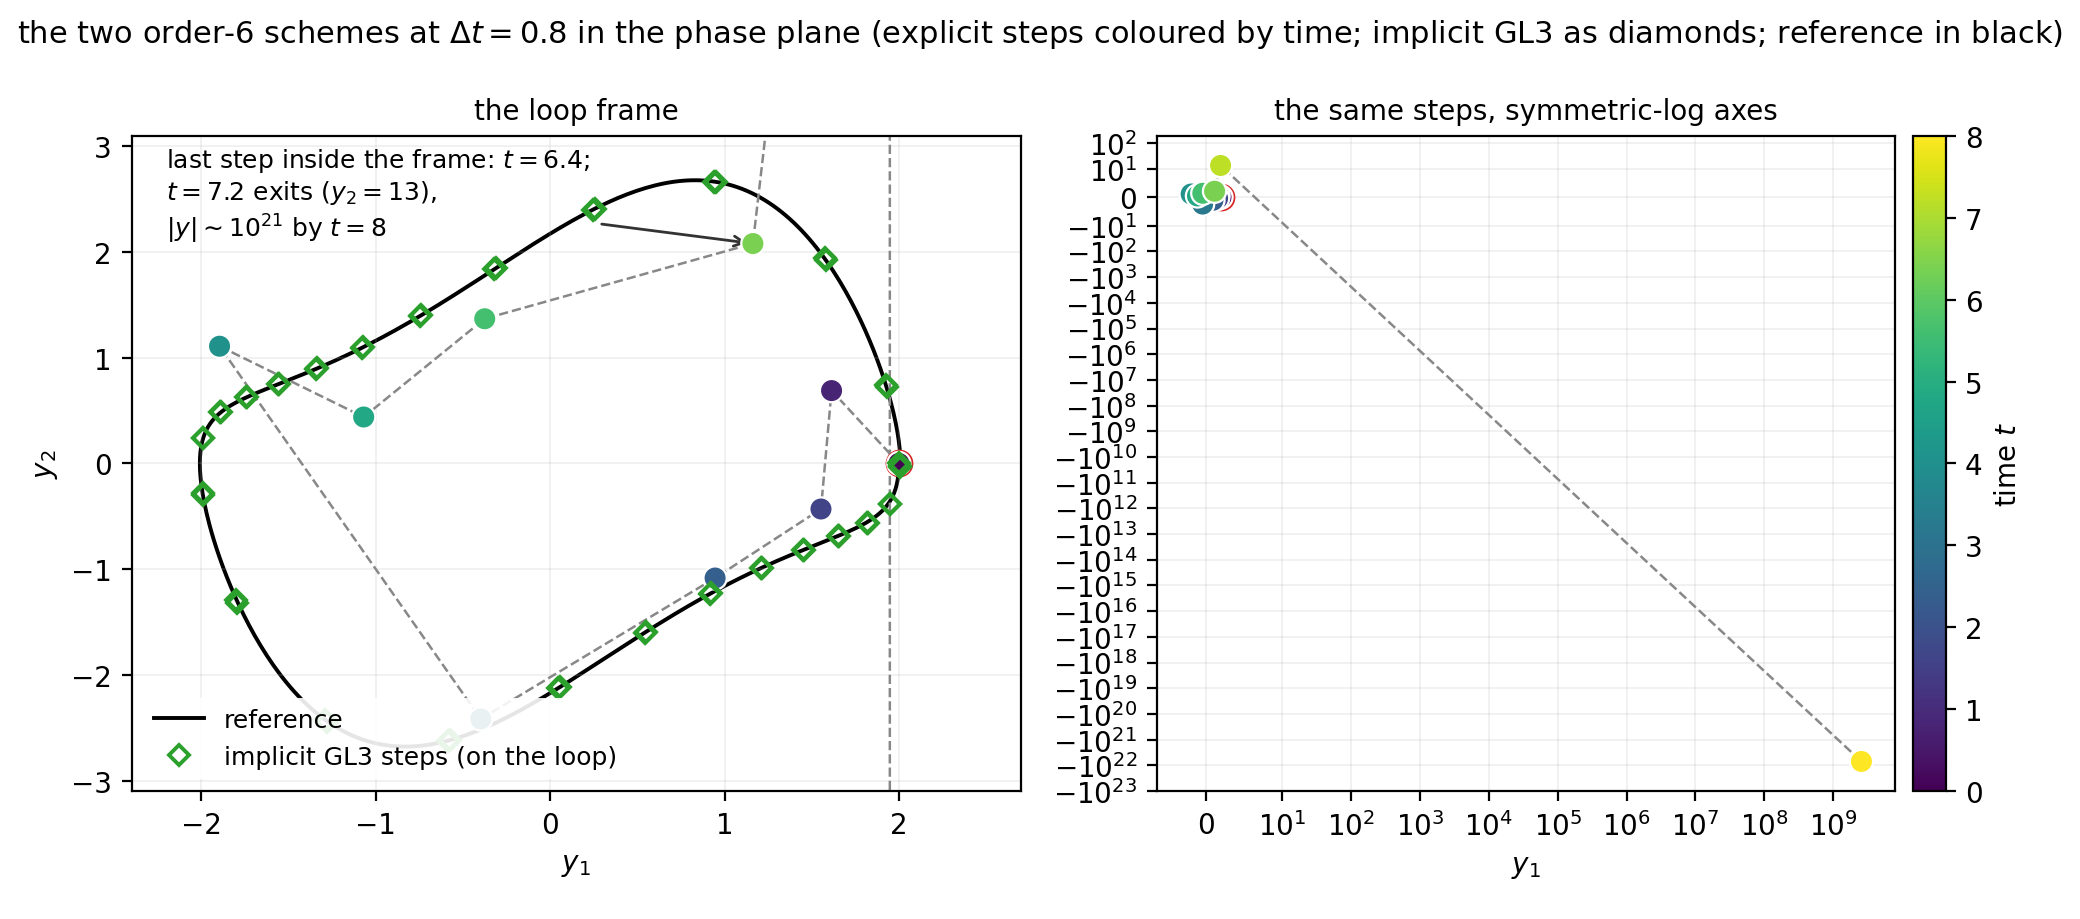
\includegraphics[width=\linewidth]{fig_rk6_phase.png}
  \caption{The classical runs of Figure~\ref{fig:rk6} in the phase
  plane, drawn as in Figure~\ref{fig:phase-collapse}: reference in
  black, the explicit RK6 steps coloured by time, the implicit
  Gauss--Legendre steps as open diamonds, the start marked in red.
  Left: the implicit steps sit on the loop all the way around, while
  the explicit steps sit off it from the outset (the first explicit
  step already reverses the sign of the velocity, $y_2 = +0.69$ where
  the reference has $-0.68$) and leave the frame after $t = 6.4$.
  Right: the explicit steps on symmetric-log axes, which is the only
  way to show the final excursion to
  $(2.6\times10^{9}, -7.1\times10^{21})$ at $t = 8$ on one pair of
  axes. Where the networks of Figure~\ref{fig:phase-collapse} leave the
  loop inward, toward the equilibrium, the explicit method at this step
  leaves it outward and does not return; the implicit method at the
  same step does not leave it at all.}
  \label{fig:rk6-phase}
\end{figure}

\begin{table}[tbp]
  \centering
  \caption{The comparison of Figure~\ref{fig:rk6} as numbers: relative
  $L_2$ error at the common step times $\{0, 0.8, \dots\} \le T$. The
  two classical columns are the explicit and implicit members of the same
  order-6 family at the same step; both runs are deterministic. Network
  entries are medians over three seeds. The step times differ from the
  dense scoring grid of Table~\ref{tab:expA}, which is why the network
  values differ slightly from that table.}
  \label{tab:rk6}
  \small
  \begin{tabular}{ccccc}
    \toprule
    $T$ & explicit RK6 & implicit GL, order 6 & plain network & causally weighted network \\
    \midrule
    3  & $0.67$      & $6.3\times10^{-5}$ & $3.3\times10^{-5}$ & $3.0\times10^{-5}$ \\
    7  & $0.72$      & $1.2\times10^{-3}$ & $6.6\times10^{-4}$ & $8.7\times10^{-5}$ \\
    14 & not finite  & $3.0\times10^{-3}$ & $0.78$             & $2.5\times10^{-4}$ \\
    27 & not finite  & $5.4\times10^{-3}$ & $0.90$             & $1.88$ \\
    40 & not finite  & $8.2\times10^{-3}$ & $0.94$             & $2.03$ \\
    \bottomrule
  \end{tabular}
\end{table}

\begin{figure}[tbp]
  \centering
  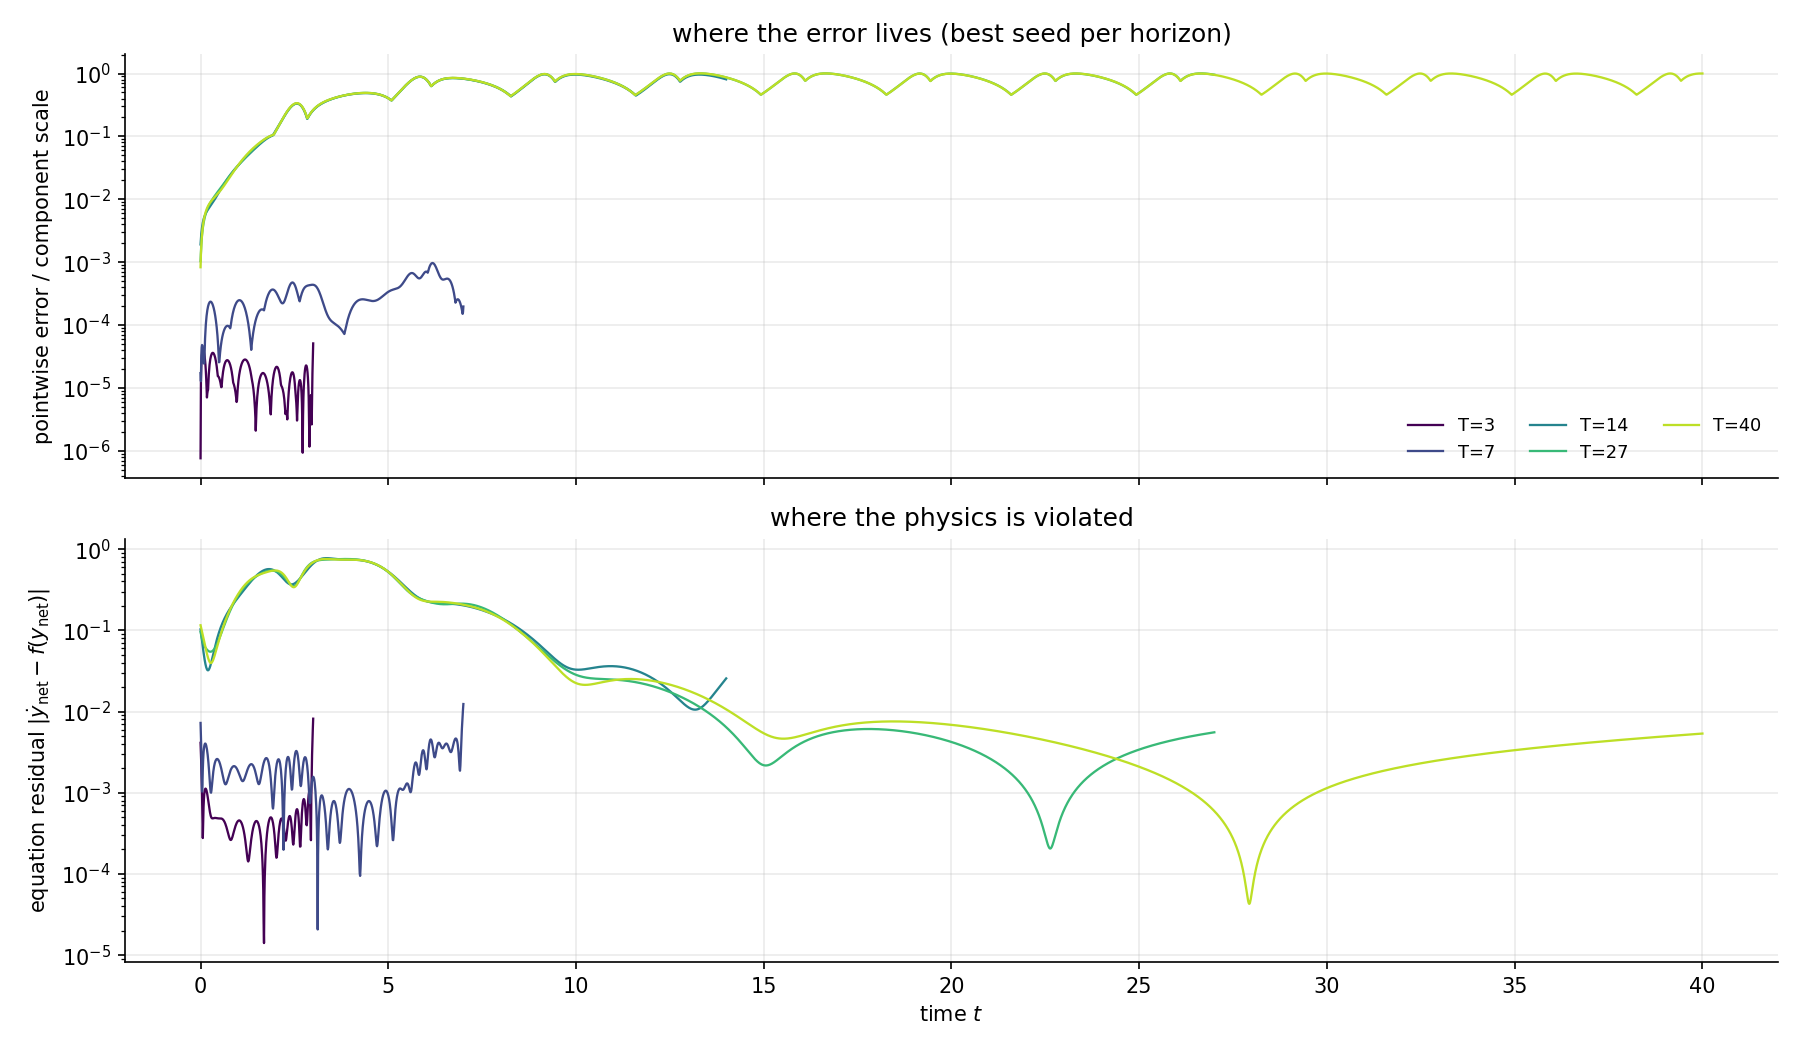
\includegraphics[width=\linewidth]{fig_diagnosis.png}
  \caption{The failure mechanism. Top: where the error lives in time
  (logarithmic scale); at the horizons past one period the error leaves
  the anchor level within the first half period, between $t \approx 1.5$
  and $3$. Bottom: the equation residual along the network's
  own trajectory. Past one period the residual is paid only in a
  short escape window and is negligible ever after: the physics is
  satisfied, on the wrong solution.}
  \label{fig:diagnosis}
\end{figure}

The mechanism is visible in Figures~\ref{fig:phase-collapse}
and~\ref{fig:diagnosis}. The origin satisfies Eq.~\eqref{eq:vdp} exactly,
so a network that parks there pays no residual at all. The true dynamics
repel from the origin, but a pointwise residual contains no stability
information, so the loss cannot distinguish the attracting truth from the
repelling impostor. The residual cost of escaping the true trajectory is
confined to a short window of fixed size, and the mean over collocation
points divides that fixed cost by the horizon, so the impostor becomes
cheaper as $T$ grows. At $T = 3$ the escape would corrupt most of the
domain and the truth wins; at $T = 14$ it costs one period out of two and
every seed falls. One $T = 40$ seed found a different escape, the
$2.09$ outlier in Table~\ref{tab:expA}.\footnote{Instead of settling at
the origin it drifted outward to $y_1 \approx 4.7$, well outside the
loop, and settled on a different wrong curve: the same mechanism with a
different destination.}

Two findings follow. First, the failure is silent: the final losses
converge to values of order $10^{-2}$ (Table~\ref{tab:expA}) while the
error is of order one, so a small, converged training loss is not evidence
of a correct solution. Second, the failure runs against
the source work's stated expectation that, for a well-posed problem with a
unique solution, good accuracy follows from a sufficiently expressive
network and sufficiently many collocation points. The problem here is
well-posed with a unique solution, the identical network fits $T = 7$, and
the collocation budget is trivially affordable and fully paid
(Section~\ref{sec:collocation}), yet the method returns the wrong solution
with a converged loss. What the loss lacks is anchoring: information about
which solution is wanted, spread across the domain instead of concentrated
at a single point. Collocation coverage is not the missing ingredient. Sections~\ref{sec:control} to~\ref{sec:axes} take this diagnosis to its conclusion: the network is shown able to represent four periods, the impostor is shown to be one member of a family of exact solutions of the equation, and the one objective that prices that family is identified and measured.

A classical integration at a comparable budget gives the comparison an
anchor (Figure~\ref{fig:rk6} and Table~\ref{tab:rk6}; the causally
weighted variant shown there is introduced in
Section~\ref{sec:causal}, and its values are included so the comparison
sits in one place). Two classical runs are shown, the explicit and
implicit members of the same order-6 family at the same step
$\Delta t = 0.8$, the step the discrete-time study of
Section~\ref{sec:disc-method} uses: the reference integrator's own
seven-stage explicit tableau, and Gauss--Legendre with $q = 3$ (also
order 6), solved by root-finding. Both are chained from the same start
and scored by the same relative $L_2$ at the common step times. The
explicit method touches $f$ at seven points per step (21 evaluations by
$T = 3$, 350 if run to $T = 40$), against the networks' 20 collocation
points per unit time re-evaluated at every epoch (up to $1{,}200$
epochs for the plain variant, up to $61{,}200$ including the Adam phase
of Section~\ref{sec:causal}); the implicit method adds a root-finding
solve per step. The findings separate three cases. The explicit method
at this step is unusable: a step of $0.8$ is far outside its stable
range on this problem, its state grows to $\sim\!10^{21}$ by $t = 8.0$
and is not finite past $t = 8.8$, and where the networks work they are
about four orders of magnitude below it ($3.3\times10^{-5}$ against
$0.67$ at $T = 3$). The implicit method of the same order at the same
step is stable at every horizon, from $6.3\times10^{-5}$ at $T = 3$ to
$8.2\times10^{-3}$ at $T = 40$; beyond two periods, where every network
fails, it is the only method in the table that still works. And within
the causally weighted variant's working range it is the network that is
more accurate for its single trained start: $3.0\times10^{-5}$ against
$6.3\times10^{-5}$ at $T = 3$, $8.7\times10^{-5}$ against
$1.2\times10^{-3}$ at $T = 7$, and $2.5\times10^{-4}$ against
$3.0\times10^{-3}$ at $T = 14$. Figure~\ref{fig:rk6-phase} shows both
runs in the phase plane, in the manner of
Figure~\ref{fig:phase-collapse}: the implicit steps sit on the loop
throughout, while the explicit steps sit off it from the outset and
leave the frame outward, where the networks' failures collapse inward.
The comparison therefore separates two different questions: at a fine
step (the reference's $h = 10^{-3}$) classical integration is better
than every network in this paper by orders of magnitude, but at the
coarse step $\Delta t = 0.8$ only implicit structure takes the step
accurately, solved classically as here or learned as in
Section~\ref{sec:disc-method}.

\subsection{Causal weighting and its limits}
\label{sec:causal}

\subsubsection{Method}

The diagnosis above is that the loss fits all times simultaneously: late
times settle onto a spurious solution before any information from the
single anchor at $t = 0$ can reach them, because nothing in
Eq.~\eqref{eq:contloss} encodes that an initial-value problem is determined
forward in time. Causal weighting~\cite{wang2024causal} encodes exactly
that and nothing else. The residual at collocation time $t_i$ is weighted
by
\begin{equation}
  w_i = \exp\!\Big(-\varepsilon \int_0^{t_i} \lVert r(s)\rVert^2 \, ds\Big),
  \label{eq:causal}
\end{equation}
with the integral evaluated as a left Riemann sum over the sorted
collocation times $t_{(1)} < t_{(2)} < \dots$: writing
$\Delta t_{(j)} = t_{(j)} - t_{(j-1)}$,
\begin{equation*}
  \int_0^{t_i} \lVert r(s)\rVert^2 \, ds \;\approx\;
  \sum_{j\,:\,t_{(j)} < t_i} \big\lVert r(t_{(j)}) \big\rVert^2\,
  \Delta t_{(j)} .
\end{equation*}
The time-weighting of the sum is deliberate: because $\varepsilon$
multiplies a time-integral rather than a bare sum over points, its
meaning is independent of collocation density, and doubling
the number of points does not double the exponent. Two different
quantities scale differently here, and it is worth separating them: the
normalisation keeps the meaning of $\varepsilon$ independent of how many
points share the domain, but the value of the integral itself still grows
with the length of trajectory being fitted, so conditions on the weights
become harder to meet as the horizon grows. This matters for the
budget-extension test below and is taken up again in the Discussion. The
weights are recomputed from the current residuals at every optimiser
iteration but treated as fixed constants by the gradient (detached from
the differentiation), so the optimiser never gains by manipulating its
own weighting. A collocation
point counts only once the trajectory \emph{before} it already satisfies
the equation: a front of solved trajectory propagates outward from the
anchor, and the far domain, where the weights are still near zero, cannot
be captured by a spurious solution in the meantime. On convergence all
residuals vanish, every weight rises to 1, and the objective becomes
exactly the plain loss, so the weighting removes itself over the course
of a successful training.

The weighting is incompatible with L-BFGS, which requires an objective
that does not change between iterations (L-BFGS builds its curvature
estimate by comparing gradients across its history, and a loss whose
weights move under it invalidates that comparison). I measured two hybrid
schedules, and both fail:
\begin{itemize}
  \item freezing the weights per L-BFGS restart lets the front advance
  only at the six refreezes; it stalled 42\% of the way across $T = 14$
  (relative error $2.15$);
  \item splitting the same 1200 epochs into 40 short restarts leaves each
  restart too short to move the front; it oscillated around 30\%
  (relative error $1.58$).
\end{itemize}
The front must move continuously; per-iteration weight updates are part of
the method. The algorithm actually used therefore follows the
causal-weighting authors:
\begin{enumerate}
  \item an Adam phase, Adam being a first-order gradient method with
  per-parameter step sizes (learning rate $10^{-3}$); each step uses the
  full batch, so steps and epochs coincide, and the weights are
  recomputed from detached residuals at every epoch;
  \item $\varepsilon$ raised through the ladder
  $\{0.01, 0.1, 1, 10, 100\}$ (small $\varepsilon$ tolerates upstream
  error; large $\varepsilon$ demands it be gone), advancing one rung
  whenever every weight exceeds $0.99$, all within a limit of
  $60{,}000$ Adam epochs; and
  \item the same L-BFGS optimisation of Section~\ref{sec:cont-protocol}
  on the plain loss, once every weight is near 1.
\end{enumerate}
I write \emph{the weight condition} for the requirement that every
weight exceed $0.99$: it is the schedule's advance condition and, at the
final $\varepsilon$ rung, the working sign that the front has crossed the
whole domain. Causal weighting thus acts as a warm start that delivers
L-BFGS into the right basin, and both variants of every comparison end by
optimising the same objective with the same optimiser. Two quantities are
logged throughout as telemetry: the minimum weight, and the fraction of
collocation points with weight above one half, written $\phi$ below.

\subsubsection{Results}

\begin{table}[tbp]
  \centering
  \caption{Plain versus causally weighted training at equal collocation
  density and architecture; medians over three seeds. The two variants
  differ in budget as well as weighting: the plain variant trains for at
  most $1{,}200$ full-batch L-BFGS epochs (a convergence criterion that
  always fired), while the causally weighted variant adds up to
  $60{,}000$ full-batch Adam epochs before an identical final L-BFGS
  phase.}
  \label{tab:causal}
  \small
  \begin{tabular}{ccccl}
    \toprule
    $T$ & periods & plain & causal & front progress (Adam epochs) \\
    \midrule
    3  & 0.45 & $3.8\times10^{-5}$ & $4.8\times10^{-5}$ & weight condition met, 3--5.5k \\
    7  & 1.05 & $6.6\times10^{-4}$ & $7.6\times10^{-5}$ & weight condition met, 8.5--28.5k \\
    14 & 2.10 & $0.79$             & $2.1\times10^{-4}$ & epoch limit reached; two seeds near $2\times10^{-4}$, third at $0.71$ \\
    27 & 4.05 & $0.90$             & $1.90$             & epoch limit reached mid-domain, all seeds ($0.88$/$1.90$/$1.99$) \\
    40 & 6.00 & $0.94$             & $2.04$             & epoch limit reached mid-domain, all seeds ($0.95$/$2.04$/$2.27$) \\
    \bottomrule
  \end{tabular}
\end{table}

\begin{figure}[tbp]
  \centering
  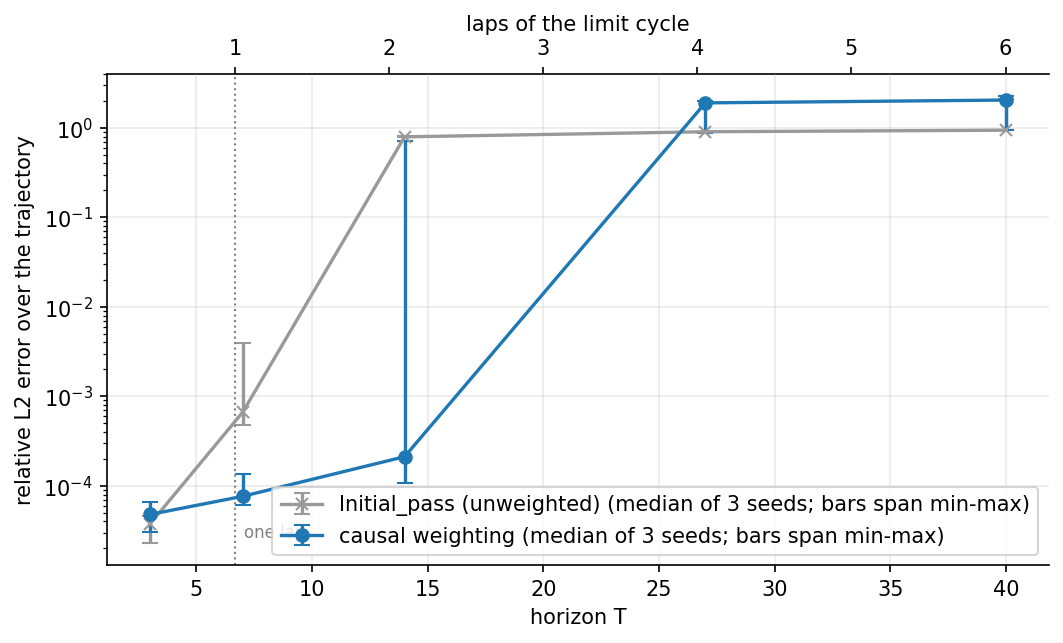
\includegraphics[width=0.8\linewidth]{fig_causal_compare.png}
  \caption{Same metric, reference and collocation density on both sides;
  the causally weighted runs additionally use the Adam phase described in
  the text. Median of three seeds with min--max
  whiskers. Causal weighting moves the horizon at which the method fails
  from between one and two periods to between two and four.}
  \label{fig:causal-compare}
\end{figure}

\begin{figure}[tbp]
  \centering
  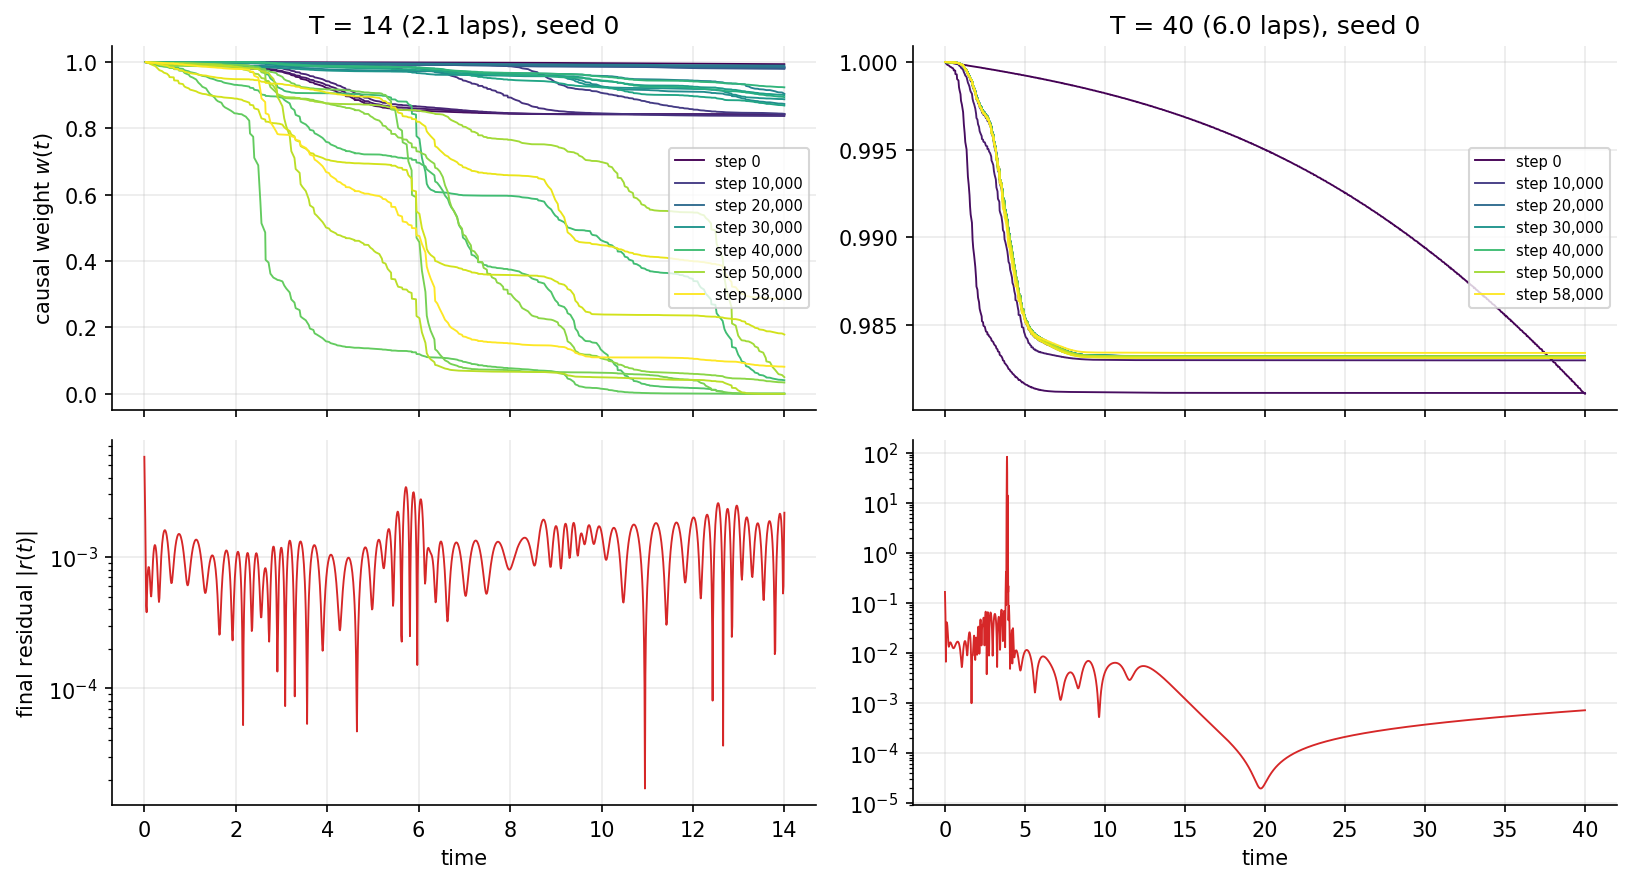
\includegraphics[width=\linewidth]{fig_causal_front.png}
  \caption{The mechanism at work: snapshots of the weight profile $w(t)$
  during training (colour: Adam epoch) at $T=14$ and $T=40$; below,
  the equation residual along the final fit. A front of large weights
  sweeps outward from the anchor as the trajectory behind it becomes
  consistent with the equation.}
  \label{fig:causal-front}
\end{figure}

Table~\ref{tab:causal} and Figure~\ref{fig:causal-compare} summarise the
comparison. At $T = 14$ (two periods, where the plain formulation
fails at $0.79$) causal weighting reaches $2.1\times10^{-4}$, an
improvement of three to four orders of magnitude; in the capped measure of
Eq.~\eqref{eq:rho} the contrast at $T=14$ is about seven orders of
magnitude (mean $\rho$ over the trajectory: $6.2\times10^{-1}$ for the
plain fit against $4.0\times10^{-8}$ for the causally weighted one,
computed from the saved run outputs). The cost of crossing the domain
grows faster than linearly:
roughly $3.5$k Adam epochs at half a period, $10$--$30$k at one
period, $60$k at two, and beyond the limit at four and six periods,
where runs stopped mid-domain score \emph{worse} than the plain
variant because the far part of the domain, its weights still near zero,
is unconstrained.
The essential difference from Section~\ref{sec:cont-results} is that
these failures are visible in the training telemetry: the minimum weight
and $\phi$ show the front still mid-domain. The plain failures, by
contrast, reported themselves as converged. One of the runs that ended at
the epoch limit also produced a second kind of silent failure, after the
collapse onto the equilibrium of Section~\ref{sec:cont-results}: a fit
with training loss $9.7\times10^{-6}$ and error $0.71$, an out-of-phase
near-solution joined to the truth by a jump inside an unsampled interval
between collocation points, invisible both to the loss and to weights
computed on the same grid. Sections~\ref{sec:density}
and~\ref{sec:placement} test directly whether more points, or
better-placed points, change these outcomes.

\subsubsection{The budget-extension test}

Every causally weighted run at $T \ge 14$ ended at the $60{,}000$-epoch
limit with its front mid-domain. So does the long-horizon failure come
down to the epoch budget? The test is direct: rerun exactly those seven
runs at $240{,}000$ epochs, four times the limit, with nothing else
changed.

\begin{table}[tbp]
  \centering
  \caption{The budget-extension test: the seven runs that reached the
  epoch limit, rerun at four times the budget. None of the seven
  completed the crossing.}
  \label{tab:extended}
  \footnotesize
  \begin{tabular}{lccl}
    \toprule
    run & 60k epochs & 240k epochs & telemetry reading \\
    \midrule
    $T=14$, seed 2 & 0.71 & 0.61 & weight condition met at 92k; still wrong (jump between points) \\
    $T=27$, seed 0 & 0.88 & 0.83 & front advancing, far slower than linearly in epochs \\
    $T=27$, seed 1 & 1.90 & 0.24 & weights saturated at small $\varepsilon$ ${\sim}185$k epochs; then $\varepsilon$ advanced \\
    $T=27$, seed 2 & 1.99 & 1.99 & no front formed; $\phi$ below 0.1 throughout \\
    $T=40$, seed 0 & 0.95 & 0.79 & front advancing, far slower than linearly in epochs \\
    $T=40$, seed 1 & 2.04 & 2.08 & weights saturated at small $\varepsilon$ for the whole run \\
    $T=40$, seed 2 & 2.27 & 2.29 & no front formed \\
    \bottomrule
  \end{tabular}
\end{table}

\begin{figure}[tbp]
  \centering
  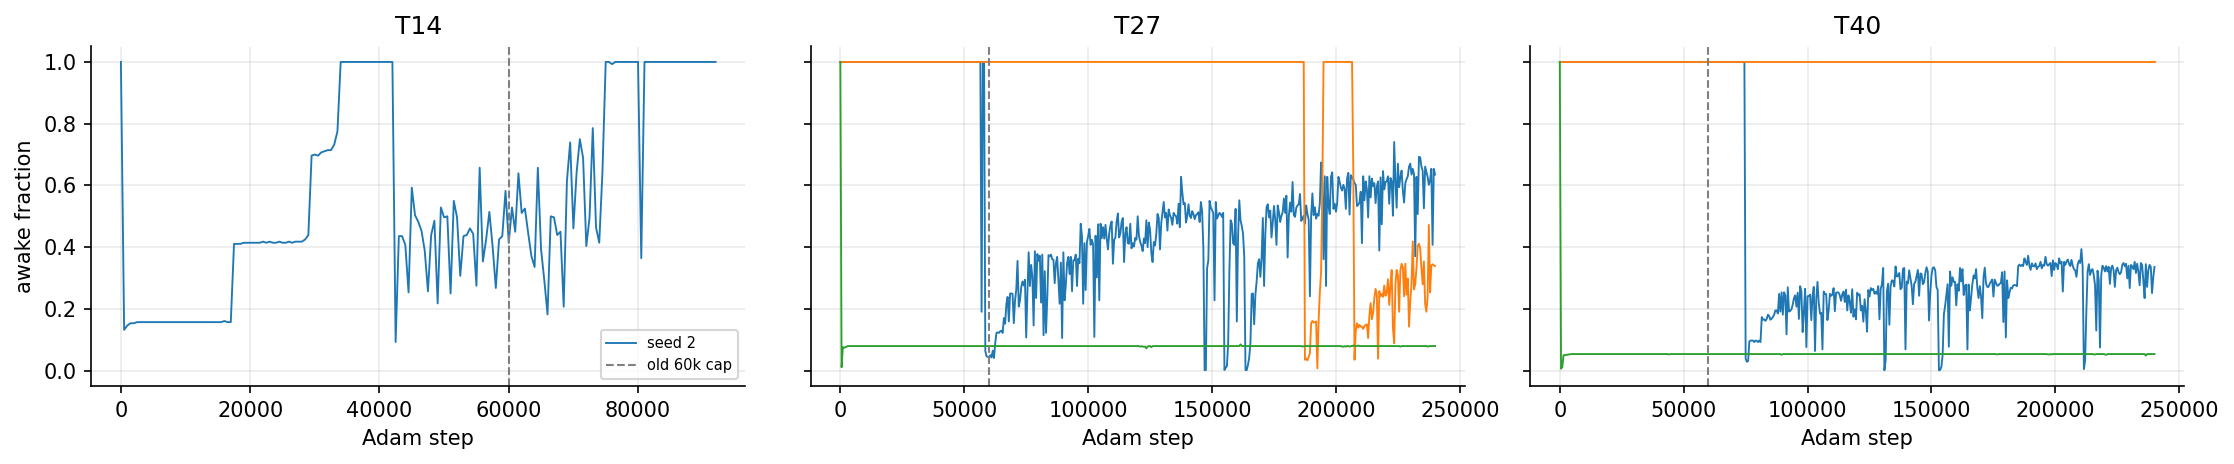
\includegraphics[width=\linewidth]{fig_telemetry.png}
  \caption{The discriminating instrument: $\phi$, the fraction of
  collocation points with weight above one half, over the extended runs,
  with the original 60k-epoch limit marked. The three outcomes described
  in the text are directly visible: a front advancing too slowly to
  finish; weights saturated at small $\varepsilon$ (note the $T=27$
  transition near 185k epochs, where $\varepsilon$ finally advances and
  the error begins to fall); and no front forming at all, $\phi$ flat
  near zero.}
  \label{fig:telemetry}
\end{figure}

\begin{figure}[tbp]
  \centering
  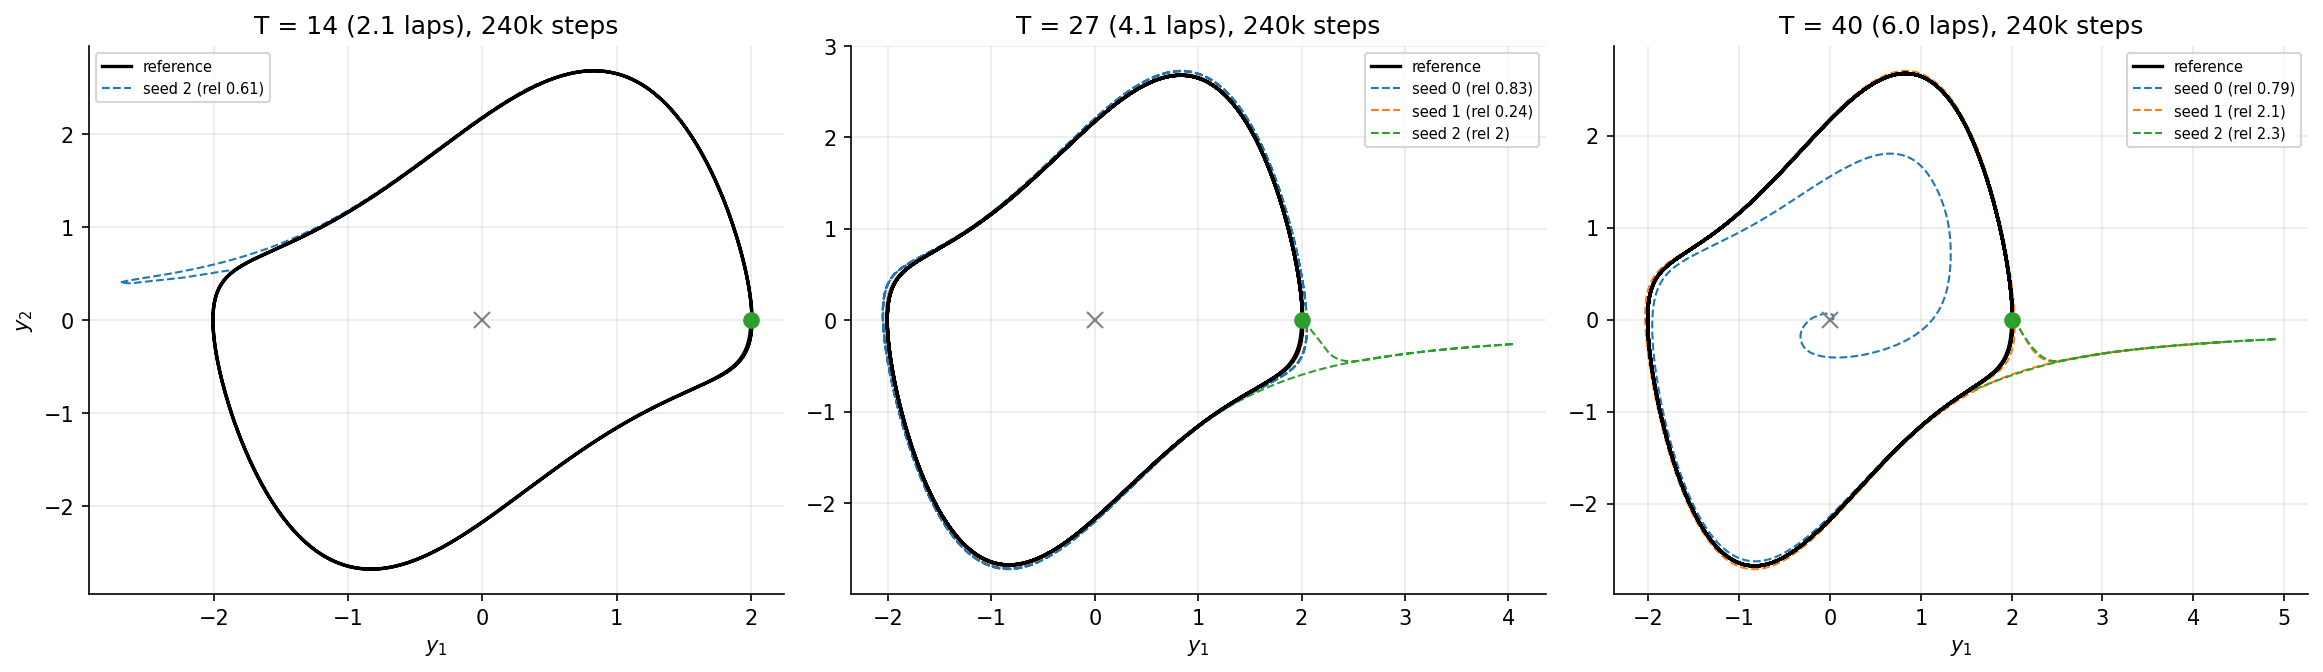
\includegraphics[width=\linewidth]{fig_extended_phase.png}
  \caption{Every extended-budget run in the phase plane. The runs whose
  weights saturated early ride the reference loop almost perfectly and
  are wrong \emph{in time}: they circulate out of phase, so the
  trajectory error is of order one while the orbit looks flawless. The
  runs where no front formed satisfy the anchor and then leave the loop.
  The one run that met the weight condition traces the loop with a
  single excursion, the jump between collocation points described in the
  text.}
  \label{fig:extended-phase}
\end{figure}

Table~\ref{tab:extended} answers the question: the original limit was
genuinely too small for some runs (one needed 92k epochs to meet the
weight condition), but four times the budget completed the crossing in
none of the seven. The telemetry (Figure~\ref{fig:telemetry}) separates
three outcomes, and the phase portraits
(Figure~\ref{fig:extended-phase}) show what each looks like as a
trajectory. In the first, the front advances but too slowly to finish
within even the extended budget. In the second, the weight condition is
never met at the first $\varepsilon$ value, so no front ever forms. In
the third, the weights saturate near 1 while $\varepsilon$ is still
small; the weighting then has little effect, training proceeds much as
if unweighted, and the fit settles on a wrong solution. The one run of
the third kind in which $\varepsilon$ eventually advanced ($T=27$,
seed 1) improved to $0.24$, still an order-one error, and the
improvement coincided with the $\varepsilon$ advance rather than with
the added epochs. The binding constraints are structural: (i) the
whole-history integral in Eq.~\eqref{eq:causal} grows with the length of
trajectory being fitted, so the weight condition becomes harder to meet
as the horizon grows, and the schedule can leave a run with no front
formed or with its weights saturated too early; and (ii) both the loss
and the weights see only the collocation grid, so a jump inside an
unsampled interval defeats even a run that met the weight condition.
Neither constraint yields to epochs at fixed collocation density.

\subsection{Network size and the starting state}
\label{sec:size-start}

The budget axis being closed, the next candidate resource is the network
itself, and with it a variable every experiment so far had frozen: the
starting state. I cross depth $\{2,4,6,8,10\}$ with width
$\{16,32,64,128,256\}$ (25 architectures), with both variants
(plain and causally weighted), two horizons ($T=14$, where the plain
variant first collapses; $T=27$, the first horizon at which the causally
weighted variant fails), and six starting
states: $(2,0)$ plus five Latin-hypercube-drawn states across the
rectangle $y_1 \in [-2.5, 2.5]$, $y_2 \in [-3, 3]$ (the limit cycle with
margin, and the same region the discrete-time formulation later trains
over), one seed each: $25 \times 2 \times 2 \times 6 = 600$ runs. Each
combination is trained once; the sweep trades seed replication for
coverage of architectures and starts, so statements below are made at
the level of 25-architecture groups or 150-run success rates, and any
single entry carries the seed-to-seed variability measured at three
seeds elsewhere in this paper.

No architecture repairs a failing horizon
(Figure~\ref{fig:size-heatmaps}). In the plain variant at $T=14$ every
architecture fails, with per-architecture medians over the six starts of
0.82--0.99 and a best single run of 0.272 across all 150; at $T=27$ the
medians are 0.93--0.98. In the causally weighted variant at $T=14$ there
is no monotonic improvement with size (best entry: depth 2, width 64,
median 0.151; most entries 0.4--1.2), and at $T=27$ the outcome is flat:
entry medians 0.86--1.22 and a best single run of 0.685. Nothing
succeeds at four periods, at any size. Two readings hold across variants
and horizons: added depth is actively harmful, and added width stops
helping beyond 64--128 units.

\begin{figure}[tbp]
  \centering
  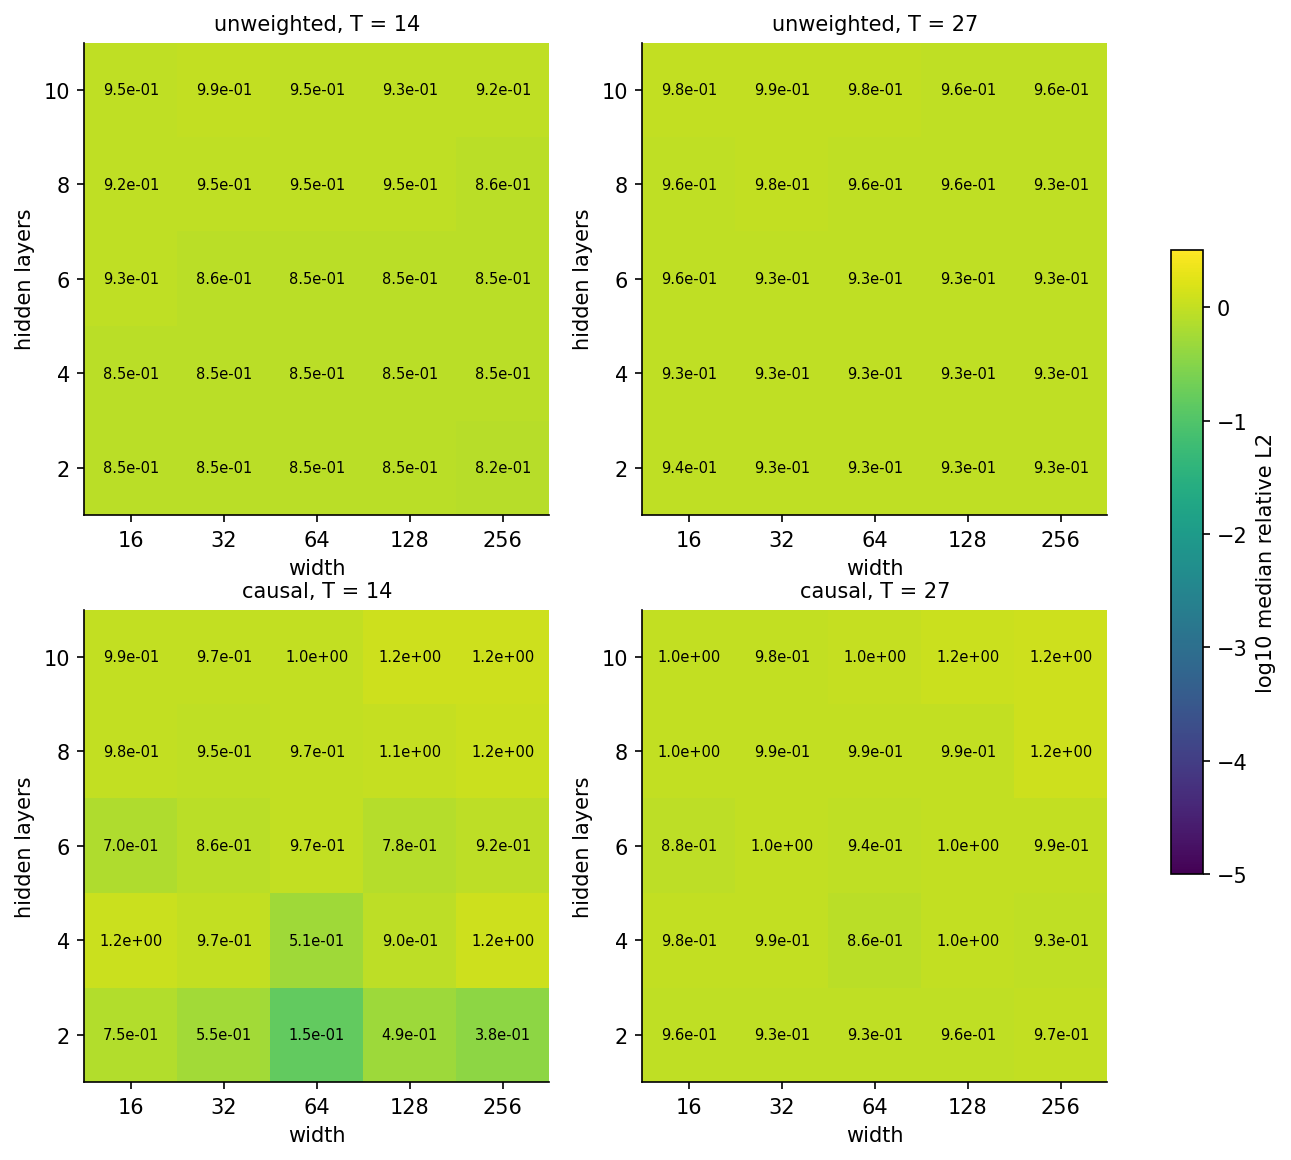
\includegraphics[width=\linewidth]{fig_size_heatmaps.png}
  \caption{Median relative $L_2$ error by architecture (depth $\times$
  width), one heatmap per variant and horizon, medians over the six
  starting states: no row or column repairs the failing horizons.
  Network size does not change where the method fails.}
  \label{fig:size-heatmaps}
\end{figure}

\begin{table}[tbp]
  \centering
  \caption{Success by starting state: causally weighted variant at $T=14$
  (two periods), counting a run a success at relative $L_2 < 10^{-2}$,
  out of the 25 architectures per start. $\lVert y^0 \rVert$ is the
  start's distance from the equilibrium at the origin; $(2,0)$ lies on
  the limit cycle.}
  \label{tab:starts}
  \small
  \begin{tabular}{cccc}
    \toprule
    start $(y_1, y_2)$ & $\lVert y^0 \rVert$ & successes / 25 & best run \\
    \midrule
    $(2.00, 0.00)$   & 2.00 & 9 & $6.7\times10^{-5}$ \\
    $(1.85, 2.90)$   & 3.45 & 6 & $1.1\times10^{-3}$ \\
    $(-2.32, -2.79)$ & 3.63 & 3 & $1.5\times10^{-3}$ \\
    $(0.87, 1.76)$   & 1.96 & 1 & $3.5\times10^{-4}$ \\
    $(-0.03, -1.02)$ & 1.02 & 0 & $1.9\times10^{-2}$ \\
    $(-0.86, -0.24)$ & 0.89 & 0 & $0.91$ \\
    \bottomrule
  \end{tabular}
\end{table}

So what does order the outcomes? The starting state
(Table~\ref{tab:starts} and Figures~\ref{fig:start-gallery}
and~\ref{fig:success-map}). Across the whole rectangle, the causally
weighted variant's success rate at the 1\% threshold is
$19/150 = 12.7\%$ at two periods and $0/150 = 0\%$ at four; the plain
variant's is 0\% at both, so at four periods none of the 300 runs of
either variant succeeds. (At a looser threshold of relative error $0.1$
the two-period count rises to 26 of 150, every one of them causally
weighted; nothing else changes.) The two inner starts, closest to the
equilibrium, never succeed; an inner start must first spiral outward
past the zero-residual solution at the origin, which an outer start
never approaches. The most successful start, $(2,0)$, is the one lying
exactly on the limit cycle; distance from the equilibrium and lying on
the cycle are confounded in this set of six starts, so I report the
counts without separating the two effects.

\begin{figure}[tbp]
  \centering
  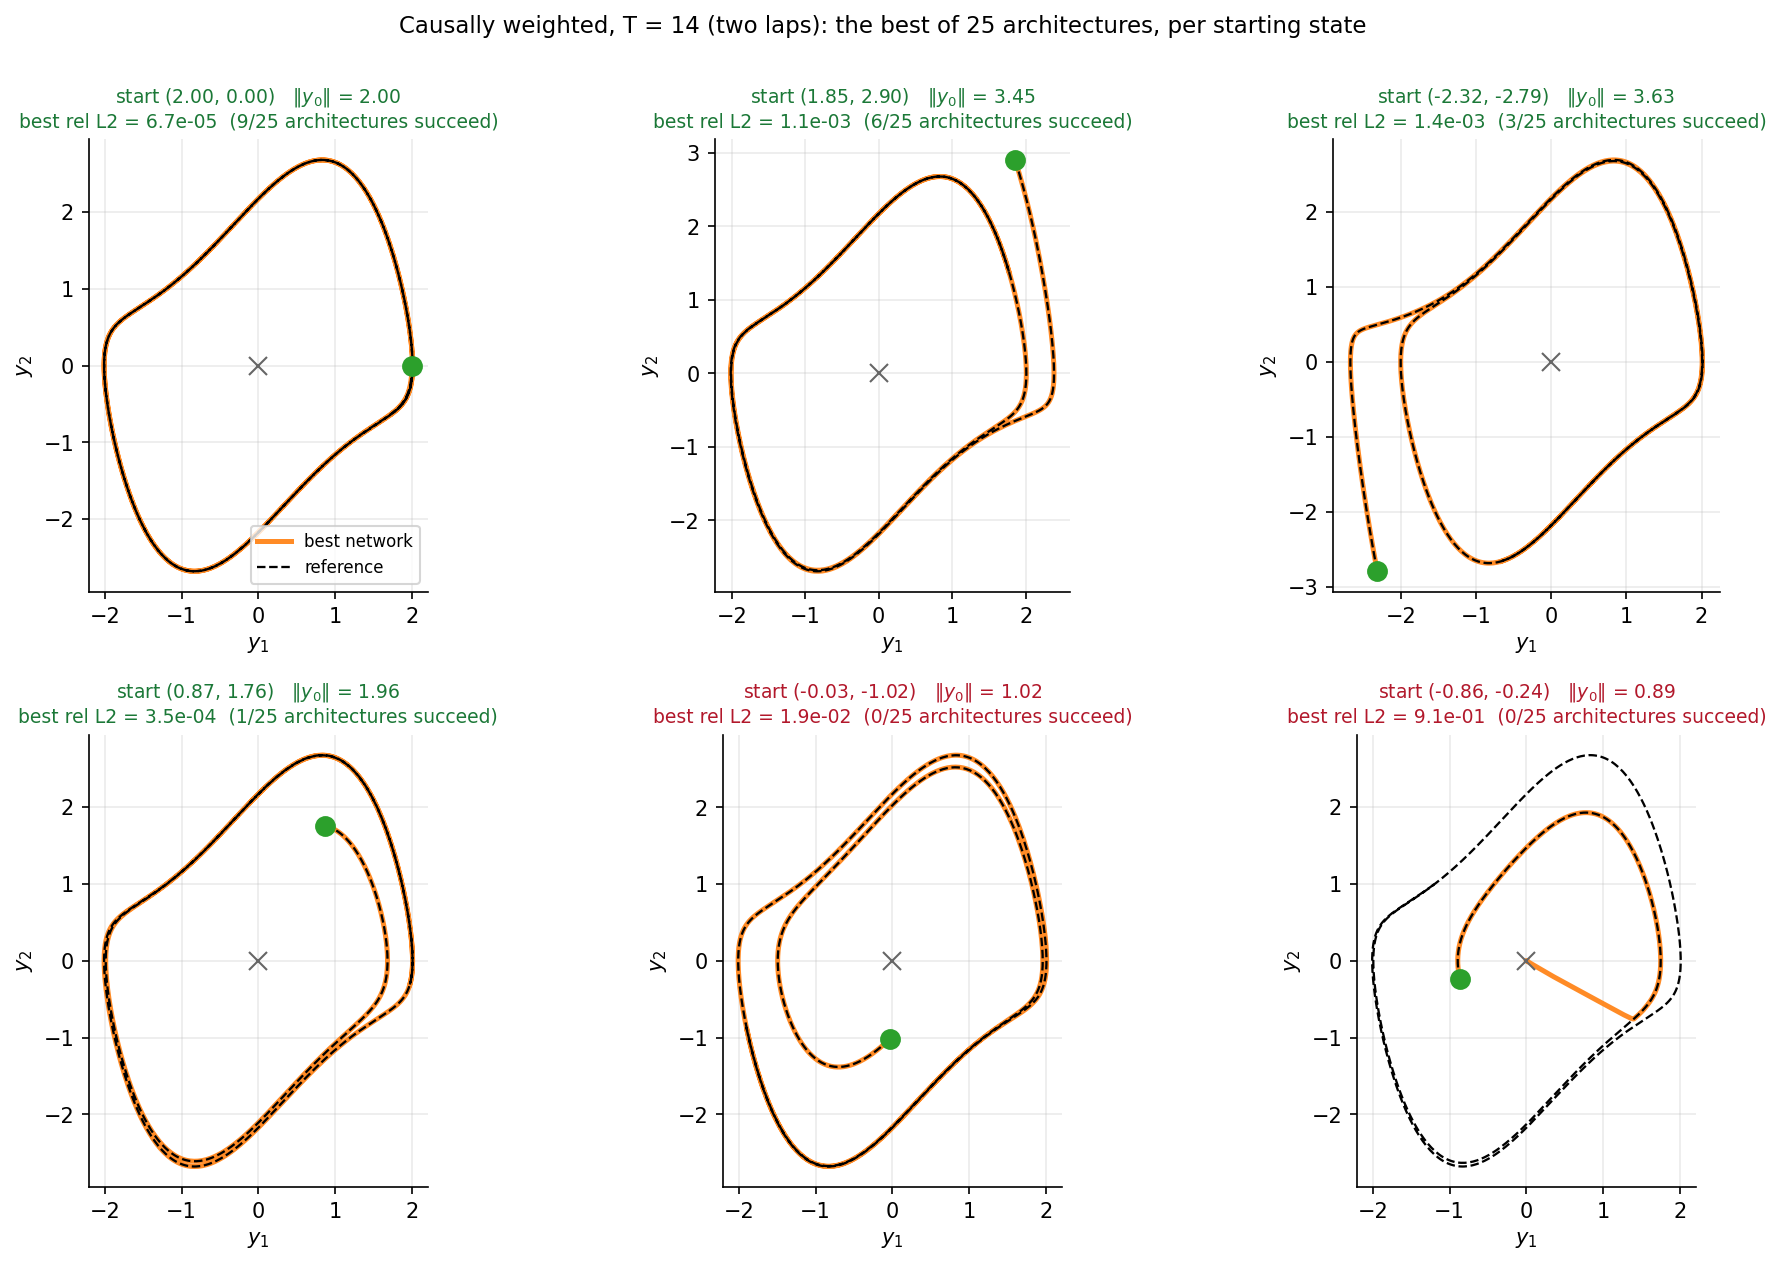
\includegraphics[width=\linewidth]{fig_start_gallery.png}
  \caption{Best causally weighted $T=14$ run (of 25 architectures) for
  each of the six starting states, in the phase plane: the outer starts
  track the loop; the two starts nearest the equilibrium are not solved
  by any architecture.}
  \label{fig:start-gallery}
\end{figure}

\begin{figure}[tbp]
  \centering
  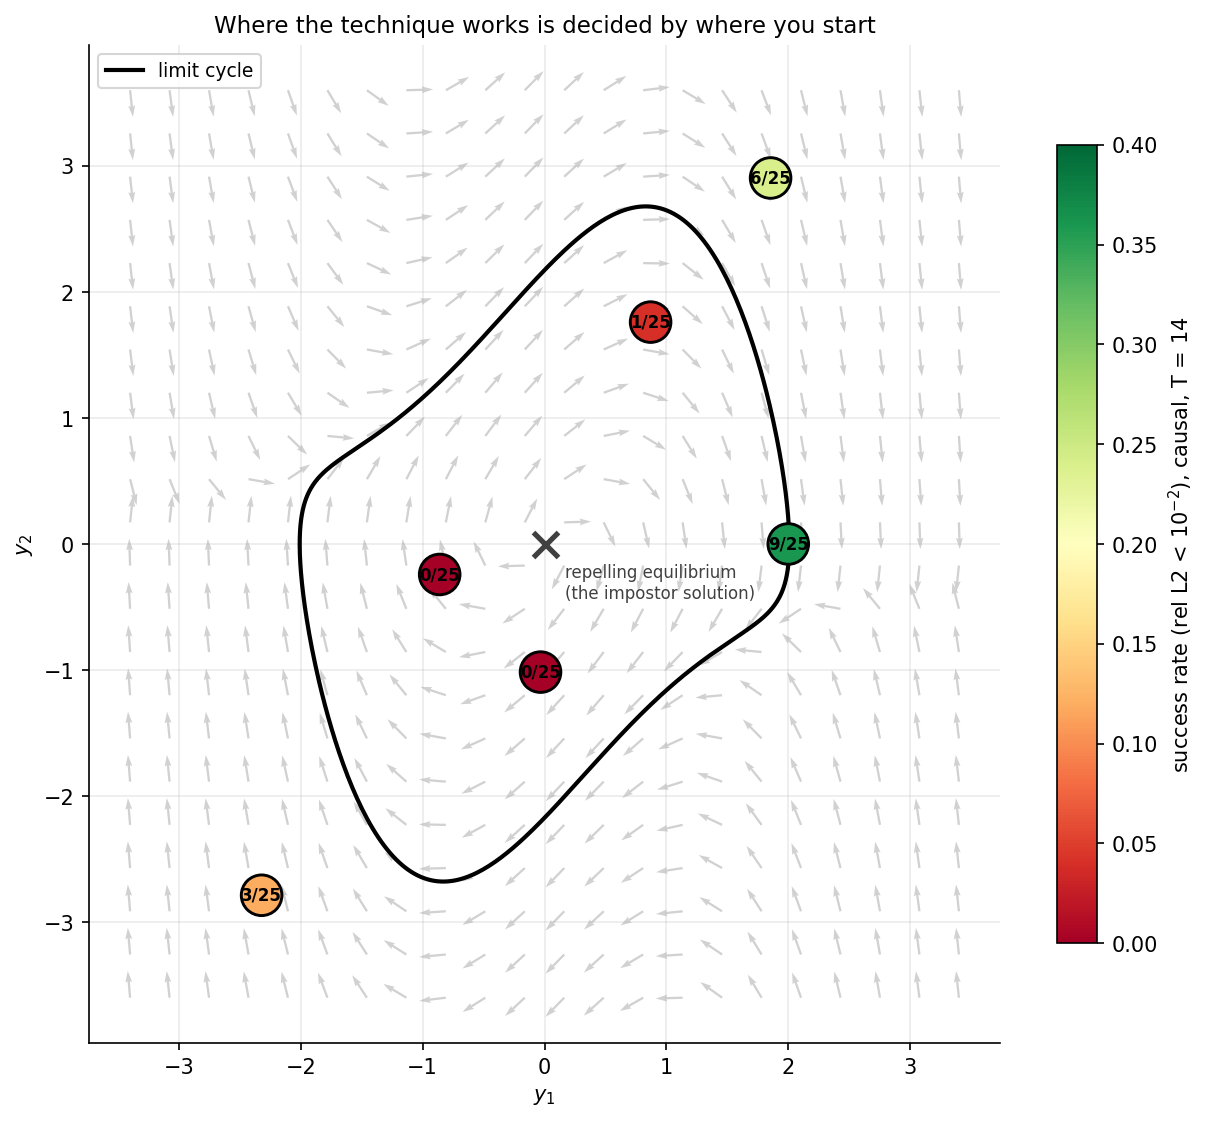
\includegraphics[width=0.72\linewidth]{fig_success_map.png}
  \caption{The six starting states drawn on the vector field, coloured by
  success count: the counts fall toward the equilibrium, and the start on
  the limit cycle is the most successful.}
  \label{fig:success-map}
\end{figure}

\subsection{Collocation density}
\label{sec:density}

The remaining resource axes are the collocation points themselves: how
many, and where. I cross densities $\{5, 80, 320\}$
points per unit time with horizons $T \in \{7, 14, 27, 40\}$, three
seeds and both variants, 72 runs; the density-20 values are those of
Sections~\ref{sec:cont-results} and~\ref{sec:causal}. I placed two
hypotheses on record before the sweep:
\begin{itemize}
  \item[H1:] the plain variant is density-independent at the horizons
  where it has failed, because the mean in Eq.~\eqref{eq:contloss}
  spreads the escape window's fixed cost over however many points share
  the domain;
  \item[H2:] the causally weighted variant is density-sensitive, through
  the unsampled intervals between collocation points
  (Section~\ref{sec:causal}).
\end{itemize}

\begin{table}[tbp]
  \centering
  \caption{Relative $L_2$ error against collocation density (points per
  unit time); medians over three seeds. ``wc'' marks runs in which the
  weight condition (every weight above 0.99) was met but the fit was
  wrong.}
  \label{tab:density}
  \small
  \begin{tabular}{clllll}
    \toprule
    variant & $T$ & $d = 5$ & $d = 20$ & $d = 80$ & $d = 320$ \\
    \midrule
    plain  & 7  & $6.4\times10^{-2}$ & $6.6\times10^{-4}$ & $9.4\times10^{-2}$ & $2.1\times10^{-3}$ \\
    plain  & 14 & $0.913$ & $0.793$ & $0.790$ & $0.792$ \\
    plain  & 27 & $0.915$ & $0.904$ & $0.905$ & $0.904$ \\
    plain  & 40 & $0.943$ & $0.942$ & $0.942$ & $0.941$ \\
    \addlinespace
    causal & 7  & $0.754$ (wc 3/3) & $7.6\times10^{-5}$ & $7.9\times10^{-5}$ & $9.7\times10^{-5}$ \\
    causal & 14 & $0.974$ (wc 2/3) & $2.1\times10^{-4}$ (worst $0.71$) & $1.8\times10^{-4}$ & $1.9\times10^{-4}$ \\
    causal & 27 & $2.70$ & $1.90$ & $1.45$ & $1.45$ \\
    causal & 40 & $2.89$ & $2.04$ & $2.05$ & $2.05$ \\
    \bottomrule
  \end{tabular}
\end{table}

H1 is confirmed at the horizons where the plain variant has failed
(Table~\ref{tab:density} and Figure~\ref{fig:density}): across a 64-fold
density range the medians at $T = 14, 27, 40$ move by factors of 1.15,
1.01 and 1.003. Collocation cost was never the binding limit there, and
this is now a direct measurement rather than an affordability argument. It is a measurement under this section's protocol, L-BFGS alone from a random start. Section~\ref{sec:axes} repeats the density axis under a protocol that trains every run to a demonstrated plateau: there density 80 lifts the plain variant at two periods from 5 of 10 seeds to 10 of 10, while at four periods and beyond it still changes nothing. H1 therefore holds at four periods and beyond, and at two periods only under the original protocol.
At $T=7$, just past one period, the plain variant sits at the margin of
its working range and the outcome is dominated by the seed rather than
the density: the medians range from $6.6\times10^{-4}$ to
$9.4\times10^{-2}$ with min--max spreads of up to three orders of
magnitude, and the variation is not monotone in density. H2 refines into
a threshold. Below roughly 20 points per unit time the weight condition
stops being informative: at density 5 it is met within about 12k Adam
epochs on wrong solutions (three of three seeds at $T=7$), because with
gaps this wide the weighting no longer orders the fit in time
(Figure~\ref{fig:density-front}). At density 20 and above, the
one-period error collapses to $\sim\!10^{-4}$ and stays flat to 320,
with a density-independent crossing cost, exactly as the $\varepsilon$
normalisation of Eq.~\eqref{eq:causal} intends. At two periods the
picture across densities is: one of three seeds at density 20 finished
at $0.71$, while at 80 and 320 all seeds landed near $2\times10^{-4}$.
The alternative placements of Section~\ref{sec:placement} also finish
three of three at density 20, so the single failing run singles out
neither the density nor the placement; I note only that every tested
change removed it. At four and six periods density changes nothing: the
causally weighted errors stay at 1.45--2.9 from 5 to 320 points per
unit time.

\begin{figure}[tbp]
  \centering
  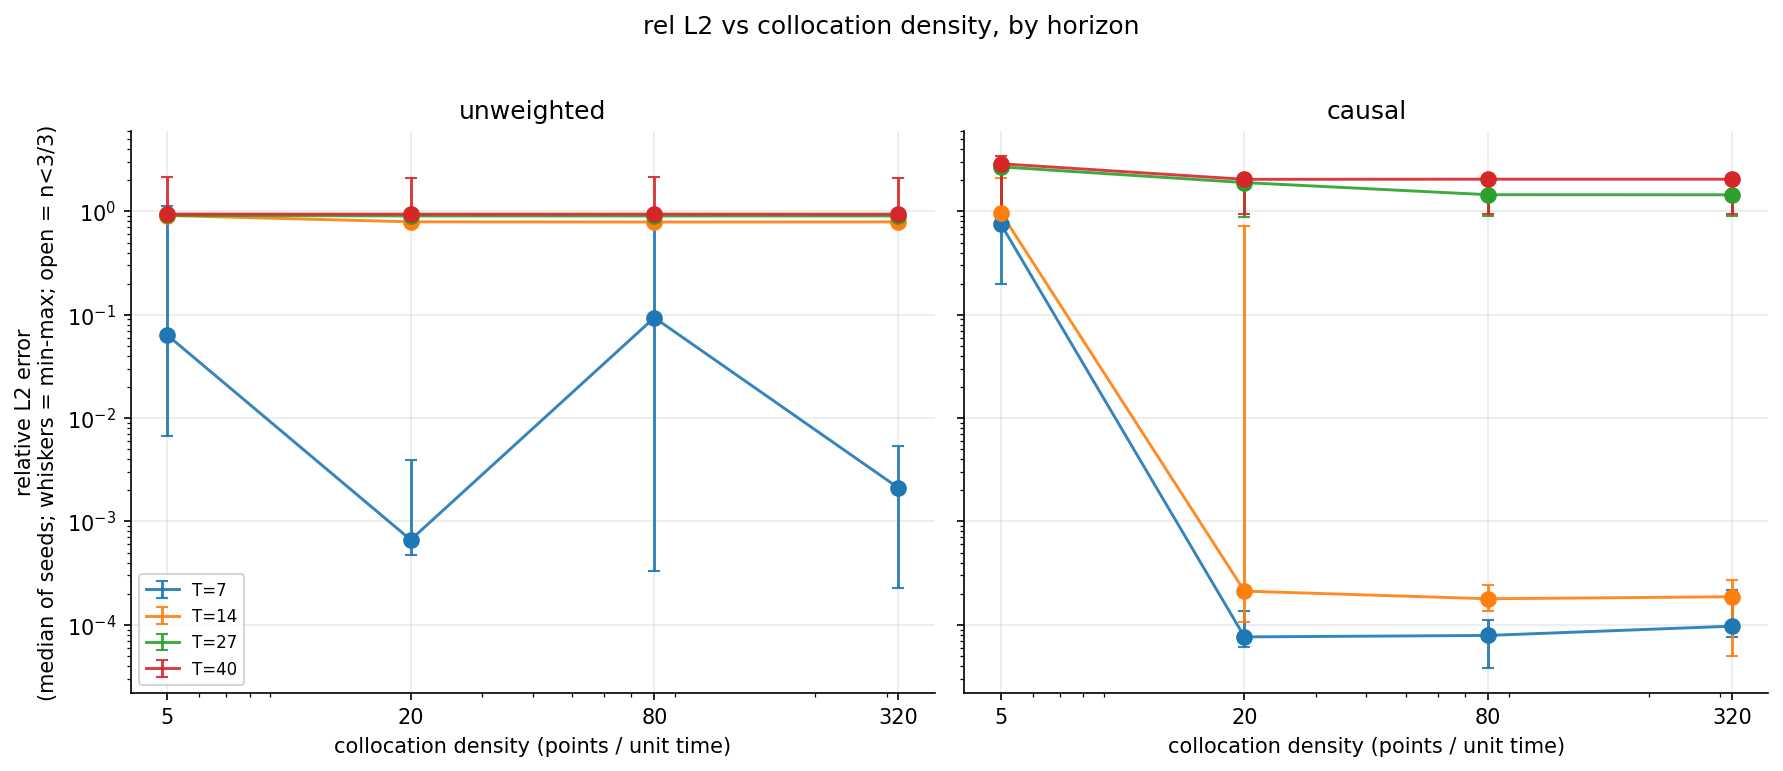
\includegraphics[width=\linewidth]{fig_density.png}
  \caption{Relative $L_2$ error against collocation density (logarithmic
  axis), one line per horizon, plain (left) and causally weighted
  (right); medians with min--max whiskers. The plain lines are flat at
  the failed horizons; the causally weighted lines drop sharply between
  density 5 and 20 at the horizons the method can reach and stay flat
  beyond, and they stay high at the horizons it cannot.}
  \label{fig:density}
\end{figure}

\begin{figure}[tbp]
  \centering
  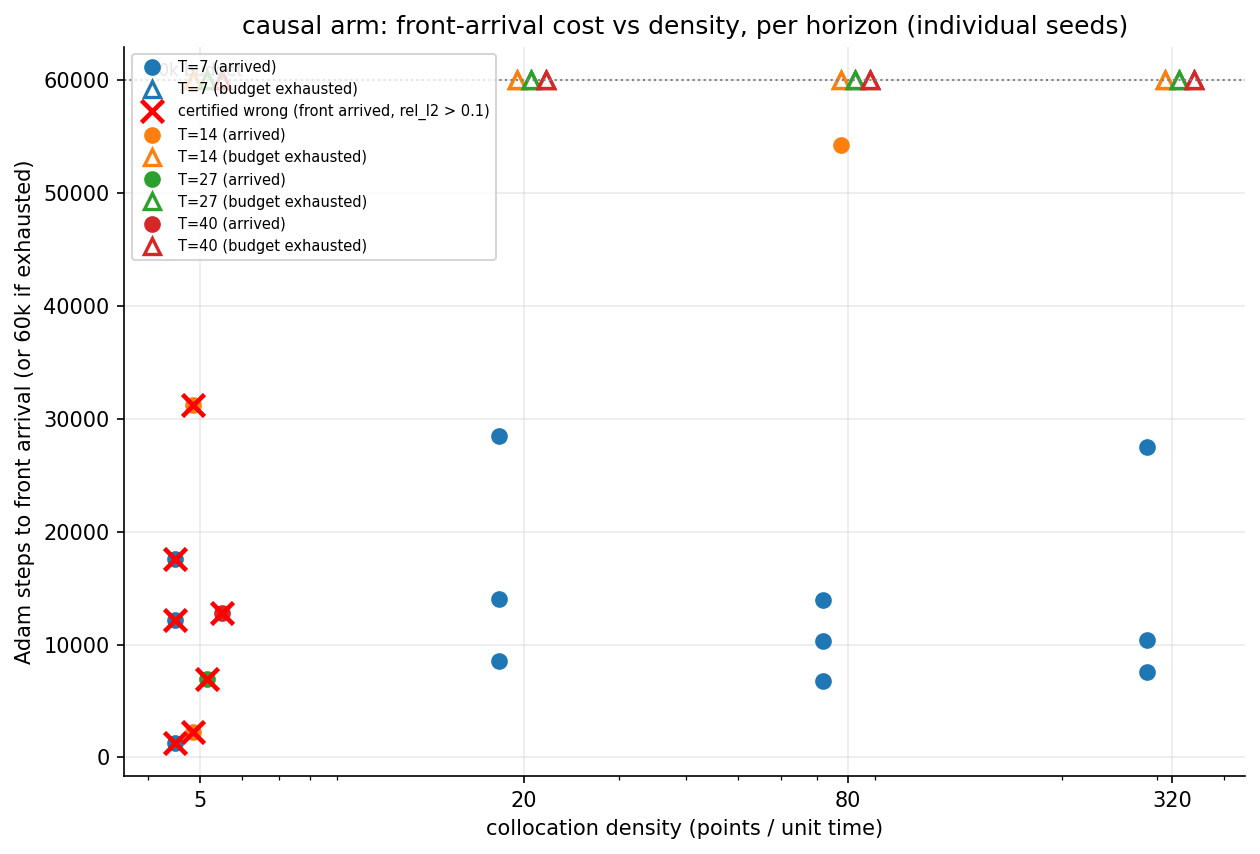
\includegraphics[width=0.8\linewidth]{fig_density_front.png}
  \caption{The Adam epochs needed to meet the weight condition, against
  density, with the wrong-solution cases marked: at density 5 the
  condition is met cheaply on wrong solutions; at density 20 and above
  the cost of meeting it is density-independent.}
  \label{fig:density-front}
\end{figure}

\subsection{Collocation placement}
\label{sec:placement}

Two kinds of escape through unsampled intervals appeared above: the
plain variant's trajectories leave the reference level within the first
half period (Figure~\ref{fig:diagnosis}, top), and one causally weighted
run at $T=14$ jumped inside an unsampled interval between collocation
points. Both raise the question of whether \emph{where} the points sit
matters. I hold the density fixed at 20 and compare two alternative
placements against the Latin-hypercube placement used everywhere else:
\emph{uniform} (deterministic bin midpoints) and \emph{anchored} (Latin
hypercube plus 40 extra points spaced geometrically inside
$(10^{-3}, 1]$, i.e.\ successive spacings in fixed ratio, concentrating
points just after the anchor), each crossed with both variants,
$T \in \{14, 27\}$ and three seeds: 24 runs.

The plain variant is placement-independent at both horizons (medians
0.786--0.806 at $T=14$, 0.901--0.910 at $T=27$, indistinguishable from
the Latin-hypercube placement). In the causally weighted variant at
$T=14$, uniform and anchored placements both finish three of three seeds
at $\le 3\times10^{-4}$ where the Latin-hypercube placement finished two
of three; a single differing run out of three cannot separate a
placement effect from seed-to-seed variability, and I report the counts
as they stand. At $T=27$ anchoring does not change the four-period
outcome: best anchored seed 0.900 (others 0.900 and 1.96); uniform
0.901, 2.85, 1.99 (Figure~\ref{fig:placement}). Concentrating points in
the interval the escapes were seen to use does not prevent the failure,
which suggests the escape is a symptom of a front that never crossed
rather than the cause of the failure. Together with
Section~\ref{sec:density} this measures the collocation axis: neither
how many points nor where they sit changes the long-horizon outcome.

\begin{figure}[tbp]
  \centering
  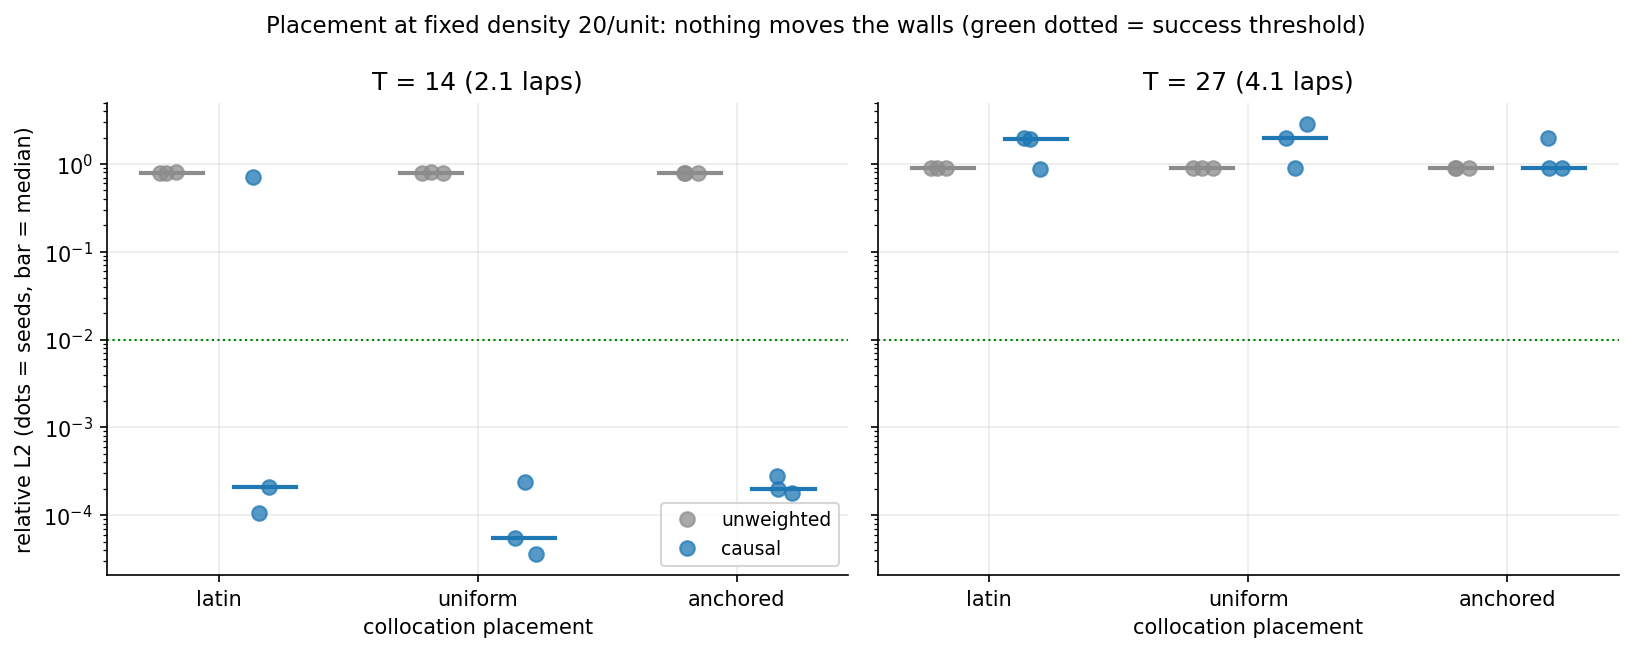
\includegraphics[width=\linewidth]{fig_placement.png}
  \caption{The placement comparison at both horizons and variants: three
  placements, indistinguishable outcomes.}
  \label{fig:placement}
\end{figure}

\subsection{The supervised control: the network is not the problem}
\label{sec:control}

Sections~\ref{sec:cont-results} to~\ref{sec:placement} leave two
suspects for the failure past two periods. Either the network and the
optimiser cannot represent four periods of the oscillation, or the
residual objective is satisfied by wrong trajectories and the optimiser
finds them. The cleanest way to separate the two is to change nothing
but the loss. I therefore trained the same networks, with the same
sample-time distribution, the same optimiser and the same caps, at
$T = 27$ on reference data alone: a plain mean squared error to the
known states at the sample times, with no residual anywhere. Four
architectures ($4\times50$, $6\times32$, $4\times64$, $10\times256$),
two sample densities (20 and 100 per unit time) and three seeds give
24 runs. The physics-trained comparison runs are those already
reported at $T = 27$: the plain variant of Section~\ref{sec:cont-results}
and the causally weighted variant of Section~\ref{sec:causal}, at the
same seeds.

\begin{figure}[tbp]
  \centering
  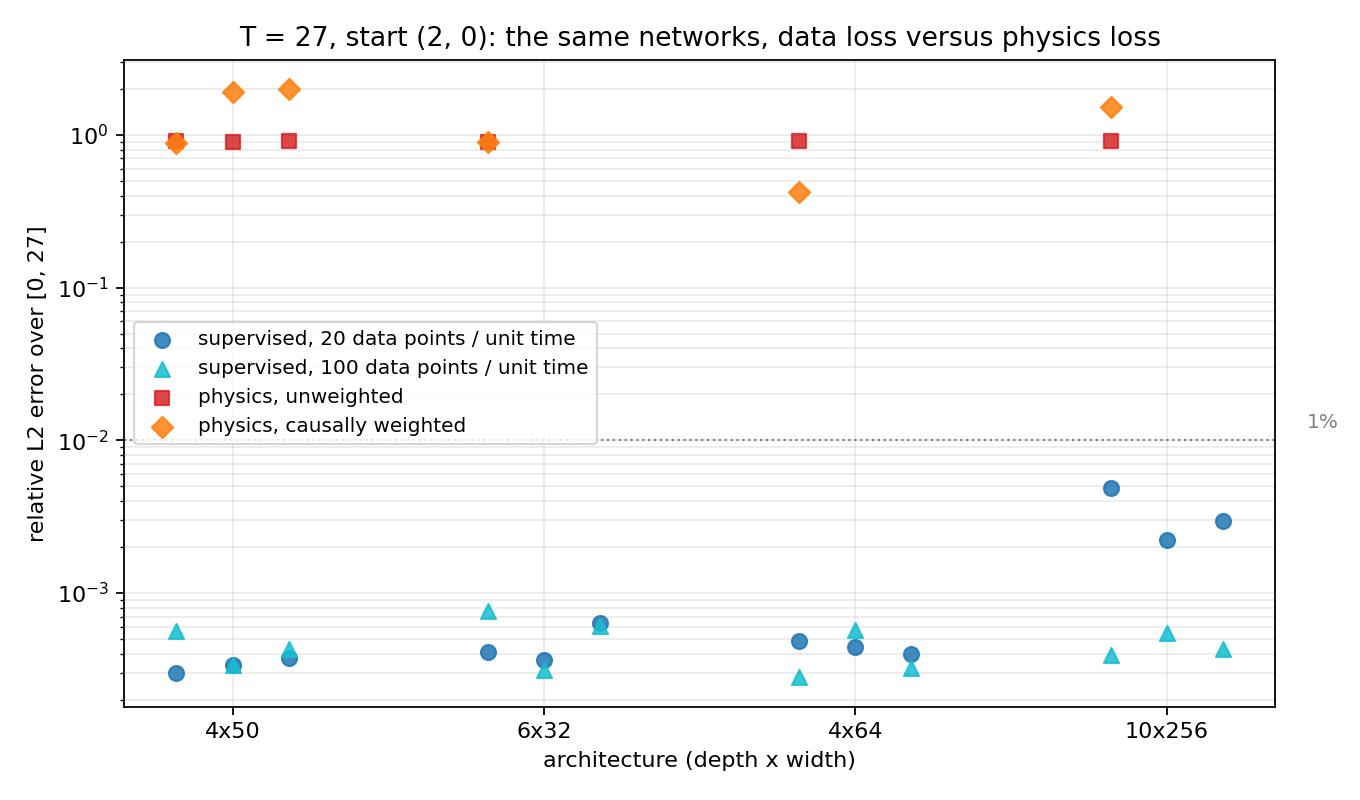
\includegraphics[width=\linewidth]{fig_control_compare.png}
  \caption{The supervised control at $T = 27$: every supervised run, at
  both sample densities, against both physics variants, by
  architecture. The separation is three to four orders of magnitude,
  with the network, the sample times and the optimiser caps held
  fixed.}
  \label{fig:control-compare}
\end{figure}

\begin{figure}[tbp]
  \centering
  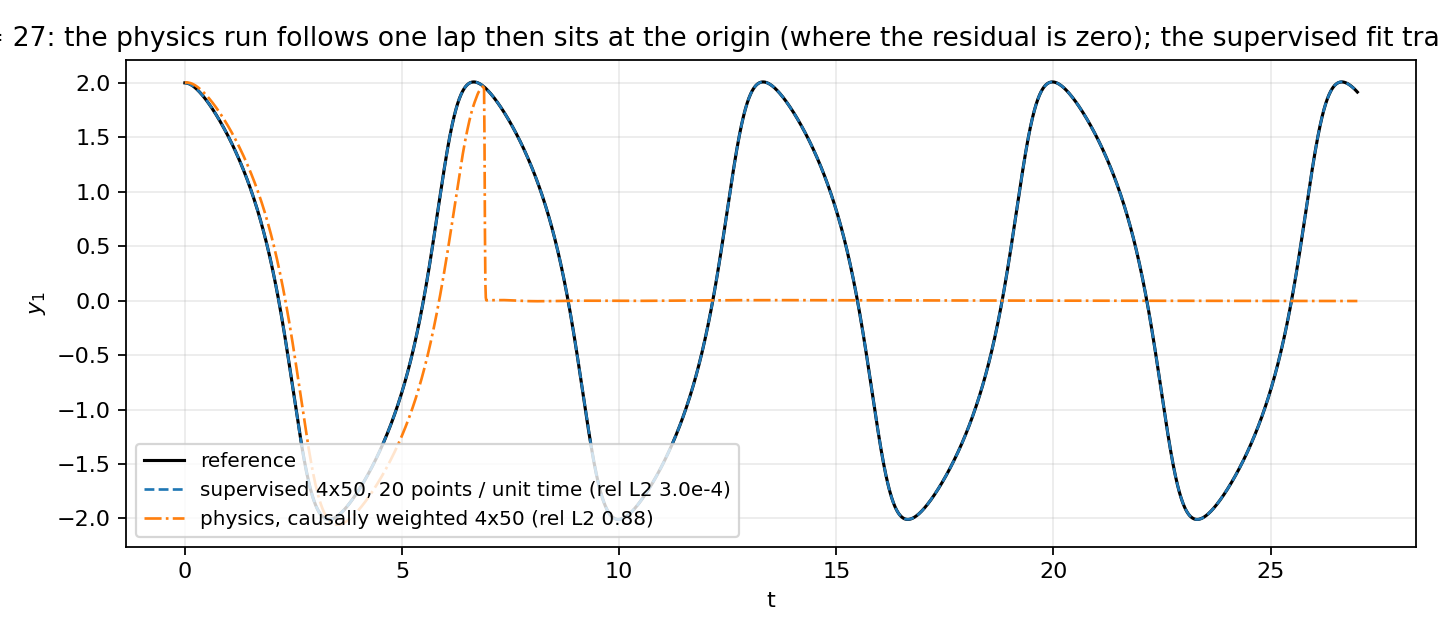
\includegraphics[width=\linewidth]{fig_control_overlay.png}
  \caption{The reference, a supervised fit at $3.0\times10^{-4}$, and a
  physics-trained run that follows one period and then sits at the
  origin for the rest of the window. The rest of this section explains
  the shape of that failure.}
  \label{fig:control-overlay}
\end{figure}

Every one of the 24 supervised runs fits four periods, at relative
$L_2$ errors between $3\times10^{-4}$ and $5\times10^{-3}$, where every
physics-trained run at the same horizon sits between $0.4$ and $2.0$
(Figures~\ref{fig:control-compare} and~\ref{fig:control-overlay}). Only
the loss changed. The network can hold four periods in phase against a
single anchor, and the optimiser can find those weights; what it cannot
do is find them through the residual. The failed physics runs follow
the reference for about one period and then sit at the origin, which is
the system's only fixed point. A constant output there has zero time
derivative and zero right-hand side, so its residual is exactly zero.
The failure is therefore a property of what the residual objective
accepts, and the next subsection works out what else it accepts. A
supervised success shows only that the network \emph{could} express the
answer; it does not say which change to the physics objective would
arrive there, which is what Section~\ref{sec:arms} tests.

\subsection{The family of spurious solutions and its price}
\label{sec:splice}

\paragraph{Fixed points are perfect minimisers.}
A fixed point of the flow is a state $y^{\ast}$ with $f(y^{\ast}) = 0$.
Van der Pol has exactly one, the origin. Its stability is read from the
Jacobian of $f$,
\begin{equation}
  J(y) = \begin{pmatrix} 0 & 1 \\ -1 - 2 y_1 y_2 & 1 - y_1^2 \end{pmatrix},
  \qquad
  J(0,0) = \begin{pmatrix} 0 & 1 \\ -1 & 1 \end{pmatrix},
  \label{eq:jacobian}
\end{equation}
whose eigenvalues at the origin solve $\lambda^2 - \lambda + 1 = 0$,
so $\lambda = \tfrac12 \pm \tfrac{\sqrt{3}}{2}\,i$. Both real parts are
$+\tfrac12$: a displacement from the origin grows like $e^{t/2}$ while
rotating, and the origin is an unstable spiral, not a saddle, a
distinction that matters for the stated limitation of the regulariser
below. If the network output is the constant $y^{\ast}$, its residual is
zero at every collocation point wherever the points sit, so the
residual term of Eq.~\eqref{eq:contloss} takes its global minimum at
every fixed point, and by continuity in the weights each fixed point
sits at the bottom of a basin. Nothing in the residual term prefers the
true solution to a constant at the origin; only the initial-condition
term does, and it is a single number set against a mean over $N$
points. This is the observation of Rohrhofer et
al.~\cite{rohrhofer2023}.

\paragraph{The splice.}
The fixed point is only the simplest member of a family. Fix the
collocation set and a time $t_0$, and let $\alpha(t)$ be a smooth
function equal to $1$ near every collocation point before $t_0$, equal
to $0$ near every collocation point after $t_0$, and equal to $0$ for
all $t \ge t_0$. The spliced candidate $y^{\dagger} = \alpha\, y^{\ast}$,
with $y^{\ast}$ now the true solution, satisfies the initial condition,
is zero after $t_0$, and has residual exactly zero at every collocation
point: near each point it coincides either with the true solution or
with the zero function, both of which solve the equation. Its residual
is nonzero only inside the \emph{transition layer}, the stretch where
$\alpha$ moves from $1$ to $0$, and that stretch has been placed between
collocation points. The empirical objective is therefore exactly zero on
$y^{\dagger}$, the value it takes on the truth. This is Theorem~2.1 of
Wang et al.~\cite{wang2026pseudo}, and its proof uses nothing about the
origin except that it solves the equation. For an autonomous system
every trajectory of the flow solves the equation, and so does every
time-shift of one, so in place of the zero function one may splice in
any trajectory $v(t)$: the candidate that follows $y^{\ast}$ near the
collocation points before $t_0$ and $v$ near those after has zero
empirical residual too. Two other members of the family appear in the
results below: the phase-shifted loop, because the residual cannot see
phase and only the anchor at $t = 0$ fixes it, and off-loop trajectories
entering from far outside the cycle. This is the exact form of the
statement made informally in Section~\ref{sec:cont-results}: the
impostors are not approximate solutions, they are exact ones, joined to
the truth where the loss cannot look.

\paragraph{What resampling changes.}
The exact zero depends on the collocation set being fixed. If fresh
points are drawn every training step the layer is eventually sampled
and its cost becomes finite. Inside a layer of width $h$ the residual is
of order $|y^{\ast}(t_0)|/h$, and the mean over the window collects that
squared over the layer,
\begin{equation}
  \frac{1}{T} \int_{\mathrm{layer}} \left| \frac{y^{\ast}(t_0)}{h} \right|^2 dt
  \;\sim\; \frac{|y^{\ast}(t_0)|^2}{h\, T}.
  \label{eq:layerprice}
\end{equation}
A hand-over from the loop to the origin taking about a period
($h \approx 2$) at amplitude $2$ in a window $T = 27$ costs of order
$4/(2 \times 27) \approx 0.07$. Three effects therefore push the same
way as $T$ grows: the price of a splice falls like $1/T$; the number of
places to put one grows like $T$; and the price of the truth rises,
because the network must hold $T/6.663$ oscillations in phase against a
single anchor. Resources such as network size or a denser fixed
collocation set change the price of representing the truth; none of
them changes the price of a splice, which is set by the objective. That
is why Sections~\ref{sec:size-start} to~\ref{sec:placement} came back
null at four periods.

\paragraph{The three papers and what each fix prices.}
Rohrhofer et al.~\cite{rohrhofer2023} supply the diagnosis: fixed points
are global minima of the physics loss with non-trivial basins, success
falls as the horizon grows and as the start approaches a fixed point, no
architecture resolves the failures, and near a fixed point the spurious
minimum can be better than the true one. They propose no remedy and do
not distinguish the fixed point from other zero-residual candidates.
Babic et al.~\cite{babic2025} add a regulariser, $C \times \frac1N
\sum_i R_{\mathrm{SE}}(t_i)\, R_{\mathrm{LS}}(t_i)$, where the
local-stability factor $R_{\mathrm{LS}} = \sum_{\lambda}
\max(\mathrm{Re}\,\lambda, 0)$ sums the positive real parts of the
eigenvalues of the Jacobian at the network's output, the stillness
factor $R_{\mathrm{SE}} = \exp(-\|\dot y_\theta\|^2/\varepsilon)$ with
$\varepsilon = 0.01$ is one only where the network's trajectory has
stopped, and the coefficient decays linearly from $0.5$ to zero at half
the training. On the true loop the slowest speed squared is $0.59$, so
the term is inert on the correct solution by construction. Their van
der Pol demonstration stops at $T = 15$, about two periods, and their
published protocol resamples 1024 collocation points every epoch, so
the published ``regularised PINN'' is the regulariser plus resampling.
Wang et al.~\cite{wang2026pseudo} prove the splice theorem above, note
that under resampling a layer of width $h$ still costs only of order
$h^{-1}$, and propose \emph{pseudo-time stepping}: the residual at
training step $k$ is replaced by a relaxed version that also penalises
change from the previous iterate,
\begin{equation}
  L_k(\theta) = \frac{1}{N} \sum_{i=1}^{N}
  \left\| \frac{y_\theta(t_i) - y_{\theta_{k-1}}(t_i)}{\tau_k}
  + r_\theta(t_i) \right\|^2 + L_{\mathrm{IC}}(\theta),
  \label{eq:pseudotime}
\end{equation}
with fresh collocation points every step, the implicit Euler
discretisation of the artificial dynamics $\partial u/\partial s =
-r[u]$ in a pseudo-time $s$. One pseudo-time update of a spliced
candidate turns its hidden layer residual of order $h^{-1}$ into order
$h^{-1} + \tau^2 h^{-3}$, an amplification by $\tau^2/h^2$, so the
relaxed objective penalises spliced candidates far more than the plain
residual does. The step $\tau$ is set adaptively from a finite-difference
surrogate of the residual Jacobian; I follow their reference code, which
produced their published numbers, where it and their text disagree on
the late-training shrink of $\tau$.

The family gives one frame for every method. A spliced candidate sits
still only if the spliced-in trajectory is the fixed point; its
transition layer is invisible on a fixed set and costs $h^{-1}$ under
resampling; and it is cheaper than the truth by a margin that shrinks
like $1/T$. Before the runs, I therefore expected the regulariser to
close exactly one member of the family, the origin, and to convert
parking into some other member at long horizons; resampling alone to
produce a parked stationary point with a loss at the layer scale, of
order $10^{-2}$; pseudo-time stepping, the only method whose mechanism
prices the whole family, to be the one to judge at $T \ge 27$; causal
weighting to delay the splice without removing its incentive; and
longer training to change nothing, because an exact minimiser cannot be
trained away, only revealed.

\subsection{Eight objectives trained to convergence}
\label{sec:arms}

\paragraph{Arms and protocol.}
All arms share the $4\times50$ network, the start $(2, 0)$, a
collocation density of 20 points per unit time, and seeds 0 to 9, at
$T \in \{14, 27, 40\}$ (2.1, 4.1 and 6.0 periods). The arms are: the
plain objective on a fixed Latin-hypercube set; the same with the
points redrawn every epoch (\emph{resample}); the regulariser with the
published dose, coefficient $0.5$ decaying to $0$ over the first 30,000
epochs; the regulariser held at $0.5$ throughout and kept in the
polish; the regulariser plus resampling, which is the published
protocol; pseudo-time stepping with the reference code's adaptive step;
causal weighting with the front propagated by Adam and $\varepsilon$
annealed from $0.01$ to $100$; and causal weighting plus the
regulariser. The regulariser is implemented as published; its
eigenvalue term was checked against a numerical eigen-decomposition and
its gradients are finite. A fixed-budget first pass of 150 runs cured
$T = 14$ but left the regularised runs at $T \ge 27$ still descending
when cut off, so every run reported here was trained to a demonstrated
plateau: Adam at learning rate $10^{-3}$ until the objective improved by
less than $10^{-4}$ over the trailing 10,000 epochs (tested only after
60,000 epochs and, for regularised arms, only once the term is off; cap
200,000), then an L-BFGS polish on the plain objective of up to 60
restarts of 200 iterations with the stall rule of Section~\ref{sec:causal}.
Every loss term is logged every 250 epochs and a per-run convergence
verdict is stored; converged and budget-limited runs are never pooled.
Of the 240 runs, 239 satisfy the rule. Every non-success is classified
from its residual on the reference grid: \emph{parked} if more than
30\,\% of the window sits within $0.2$ of the origin;
\emph{flow-following} if the residual is below $0.05$ on at least
60\,\% of the window with a peak above $1$, the signature of a splice;
\emph{diffuse} otherwise.

\begin{table}[tbp]
  \centering
  \caption{Eight objectives at two, four and six periods, ten seeds
  each, every run trained to a demonstrated plateau and polished to a
  stall. Success is relative $L_2 < 0.15$ over the window, the threshold
  of the two Graz papers. The last column classifies the failures past
  two periods (counts at $T = 27$; $T = 40$ in parentheses).}
  \label{tab:arms}
  \footnotesize
  \resizebox{\linewidth}{!}{%
  \begin{tabular}{lcccll}
    \toprule
    arm & $T=14$ & $T=27$ & $T=40$ & median rel.\ $L_2$, $T=27$ / $40$ & failures past two periods \\
    \midrule
    plain & 5/10 & 0/10 & 0/10 & $0.95$ / $0.94$ & parked 9, diffuse 1 (10 parked) \\
    resample & 10/10 & 0/10 & 0/10 & $0.90$ / $0.94$ & parked 10 at loss $0.02$--$0.03$ (10) \\
    regulariser & 10/10 & 0/10 & 0/10 & $2.2$ / $3.6$ & flow-following 6, diffuse 3, parked 1 (7, 3) \\
    regulariser always on & 10/10 & 0/10 & 0/10 & $1.9$ / $2.7$ & flow-following 8, diffuse 2 (5, 5) \\
    regulariser + resampling & 10/10 & 0/10 & 0/10 & $1.7$ / $2.6$ & flow-following 6, diffuse 4 (5, 5) \\
    pseudo-time stepping & 10/10 & \textbf{8/10} & \textbf{7/10} & $\mathbf{5.2\times10^{-4}}$ / $\mathbf{5.4\times10^{-3}}$ & parked 2 (parked 2, diffuse 1) \\
    causal & 8/10 & 0/10 & 0/10 & $1.9$ / $2.1$ & parked 2, flow-following 4, diffuse 4 \\
    causal + regulariser & 7/10 & 0/10 & 0/10 & $2.2$ / $2.1$ & flow-following 7, diffuse 2, parked 1 \\
    \bottomrule
  \end{tabular}}
\end{table}

\begin{figure}[tbp]
  \centering
  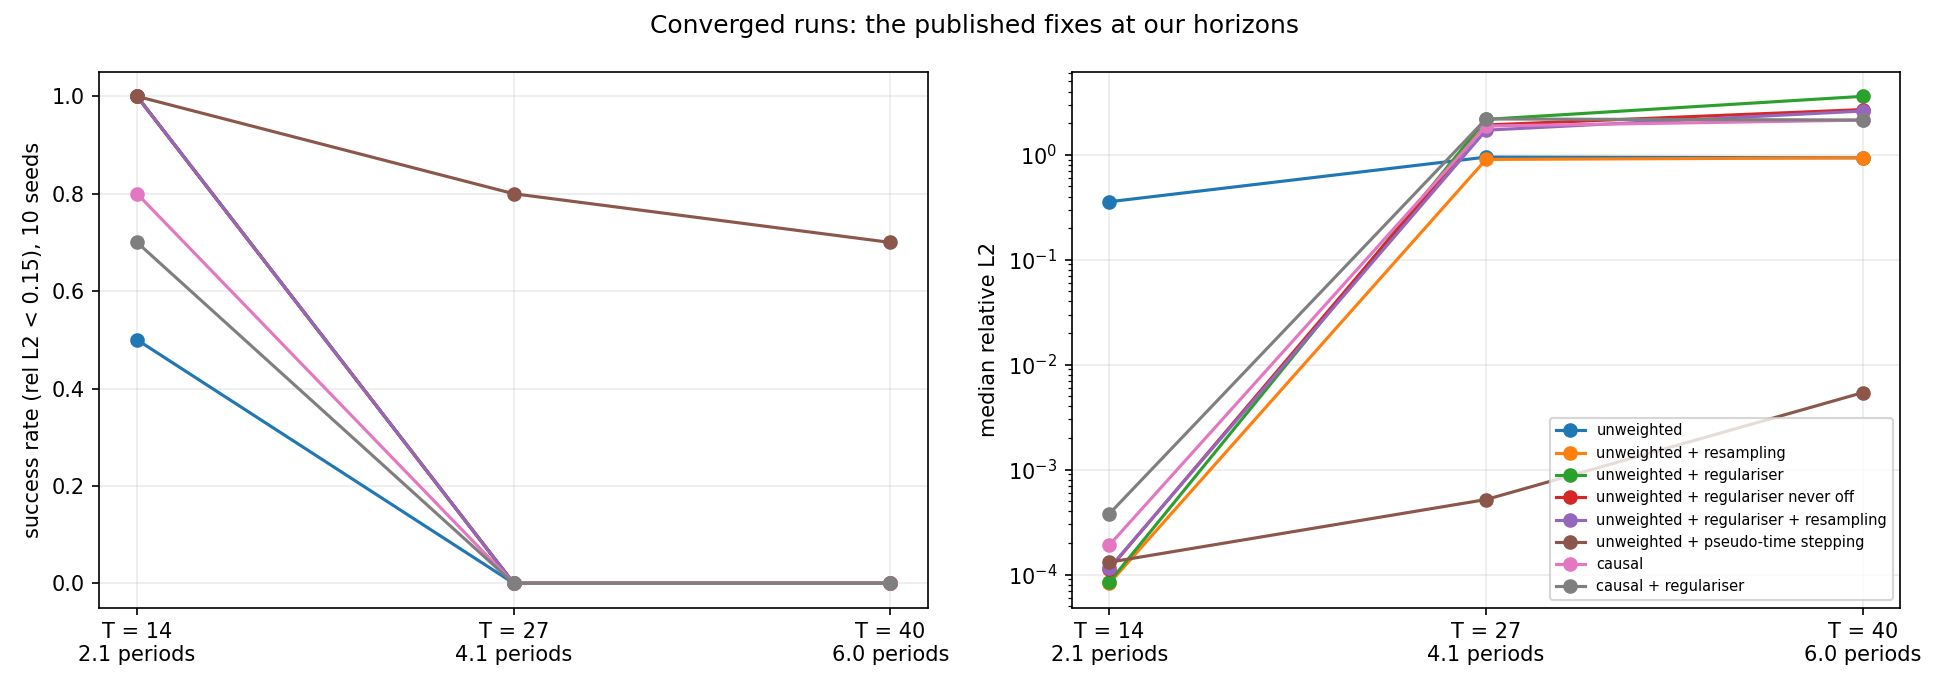
\includegraphics[width=\linewidth]{fig_arms_summary.png}
  \caption{Success rate (left) and median relative $L_2$ (right) per
  arm and horizon, ten seeds per point. Every arm reaches two periods;
  only pseudo-time stepping survives past them.}
  \label{fig:arms-summary}
\end{figure}

\paragraph{Results.}
Table~\ref{tab:arms} and Figure~\ref{fig:arms-summary} give the
headline. Every fix works at two periods, where the regulariser paper
tested it: the plain objective's 5 of 10 becomes 10 of 10 under
resampling, under the regulariser, or under pseudo-time stepping. Past
two periods every arm is 0 of 10 except pseudo-time stepping, whose
eight successes at four periods span $8.5\times10^{-5}$ to
$8.4\times10^{-4}$ and whose seven at six periods span
$4.2\times10^{-4}$ to $8.9\times10^{-3}$; its adaptive step settled
between $0.5$ and $0.9$ in every run. The failures divide into the
three classes predicted above (Figures~\ref{fig:arms-traj}
to~\ref{fig:arms-residual}). The plain and resampled objectives park at
the origin after about one period; the fixed-set parks reach the same
loss as a success, and the resampled parks sit at a loss of $0.02$ to
$0.03$ with zero gradient, the stationary point at the layer scale that
Eq.~\eqref{eq:layerprice} predicts. Every regulariser variant instead
converges onto a spliced off-loop trajectory: the residual is below
$0.05$ on more than 95\,\% of the window with one spike of $10^2$ to
$10^3$ immediately after $t = 0$, the network satisfies the anchor,
splices within the first unsampled gap onto a trajectory of the flow
entering from $y_1 \approx 4.5$, and rides it onto the loop out of
phase, with a converged loss of $10^{-5}$ to $10^{-4}$. The regulariser
closed the origin and the optimiser took the next-cheapest member of
the family; keeping the term on, or adding resampling to it, changes
nothing, as expected. The loss-term curves
(Figure~\ref{fig:arms-lossterms}) add two facts: in the regularised arms
the raw regulariser value rises after switch-off while the objective
keeps falling, and the polish drives the flow-following objectives
below $10^{-4}$ without moving the error at all. Loss and error
decouple on that branch, which is the silent failure of
Section~\ref{sec:cont-results} in its converged form.

\begin{figure}[tbp]
  \centering
  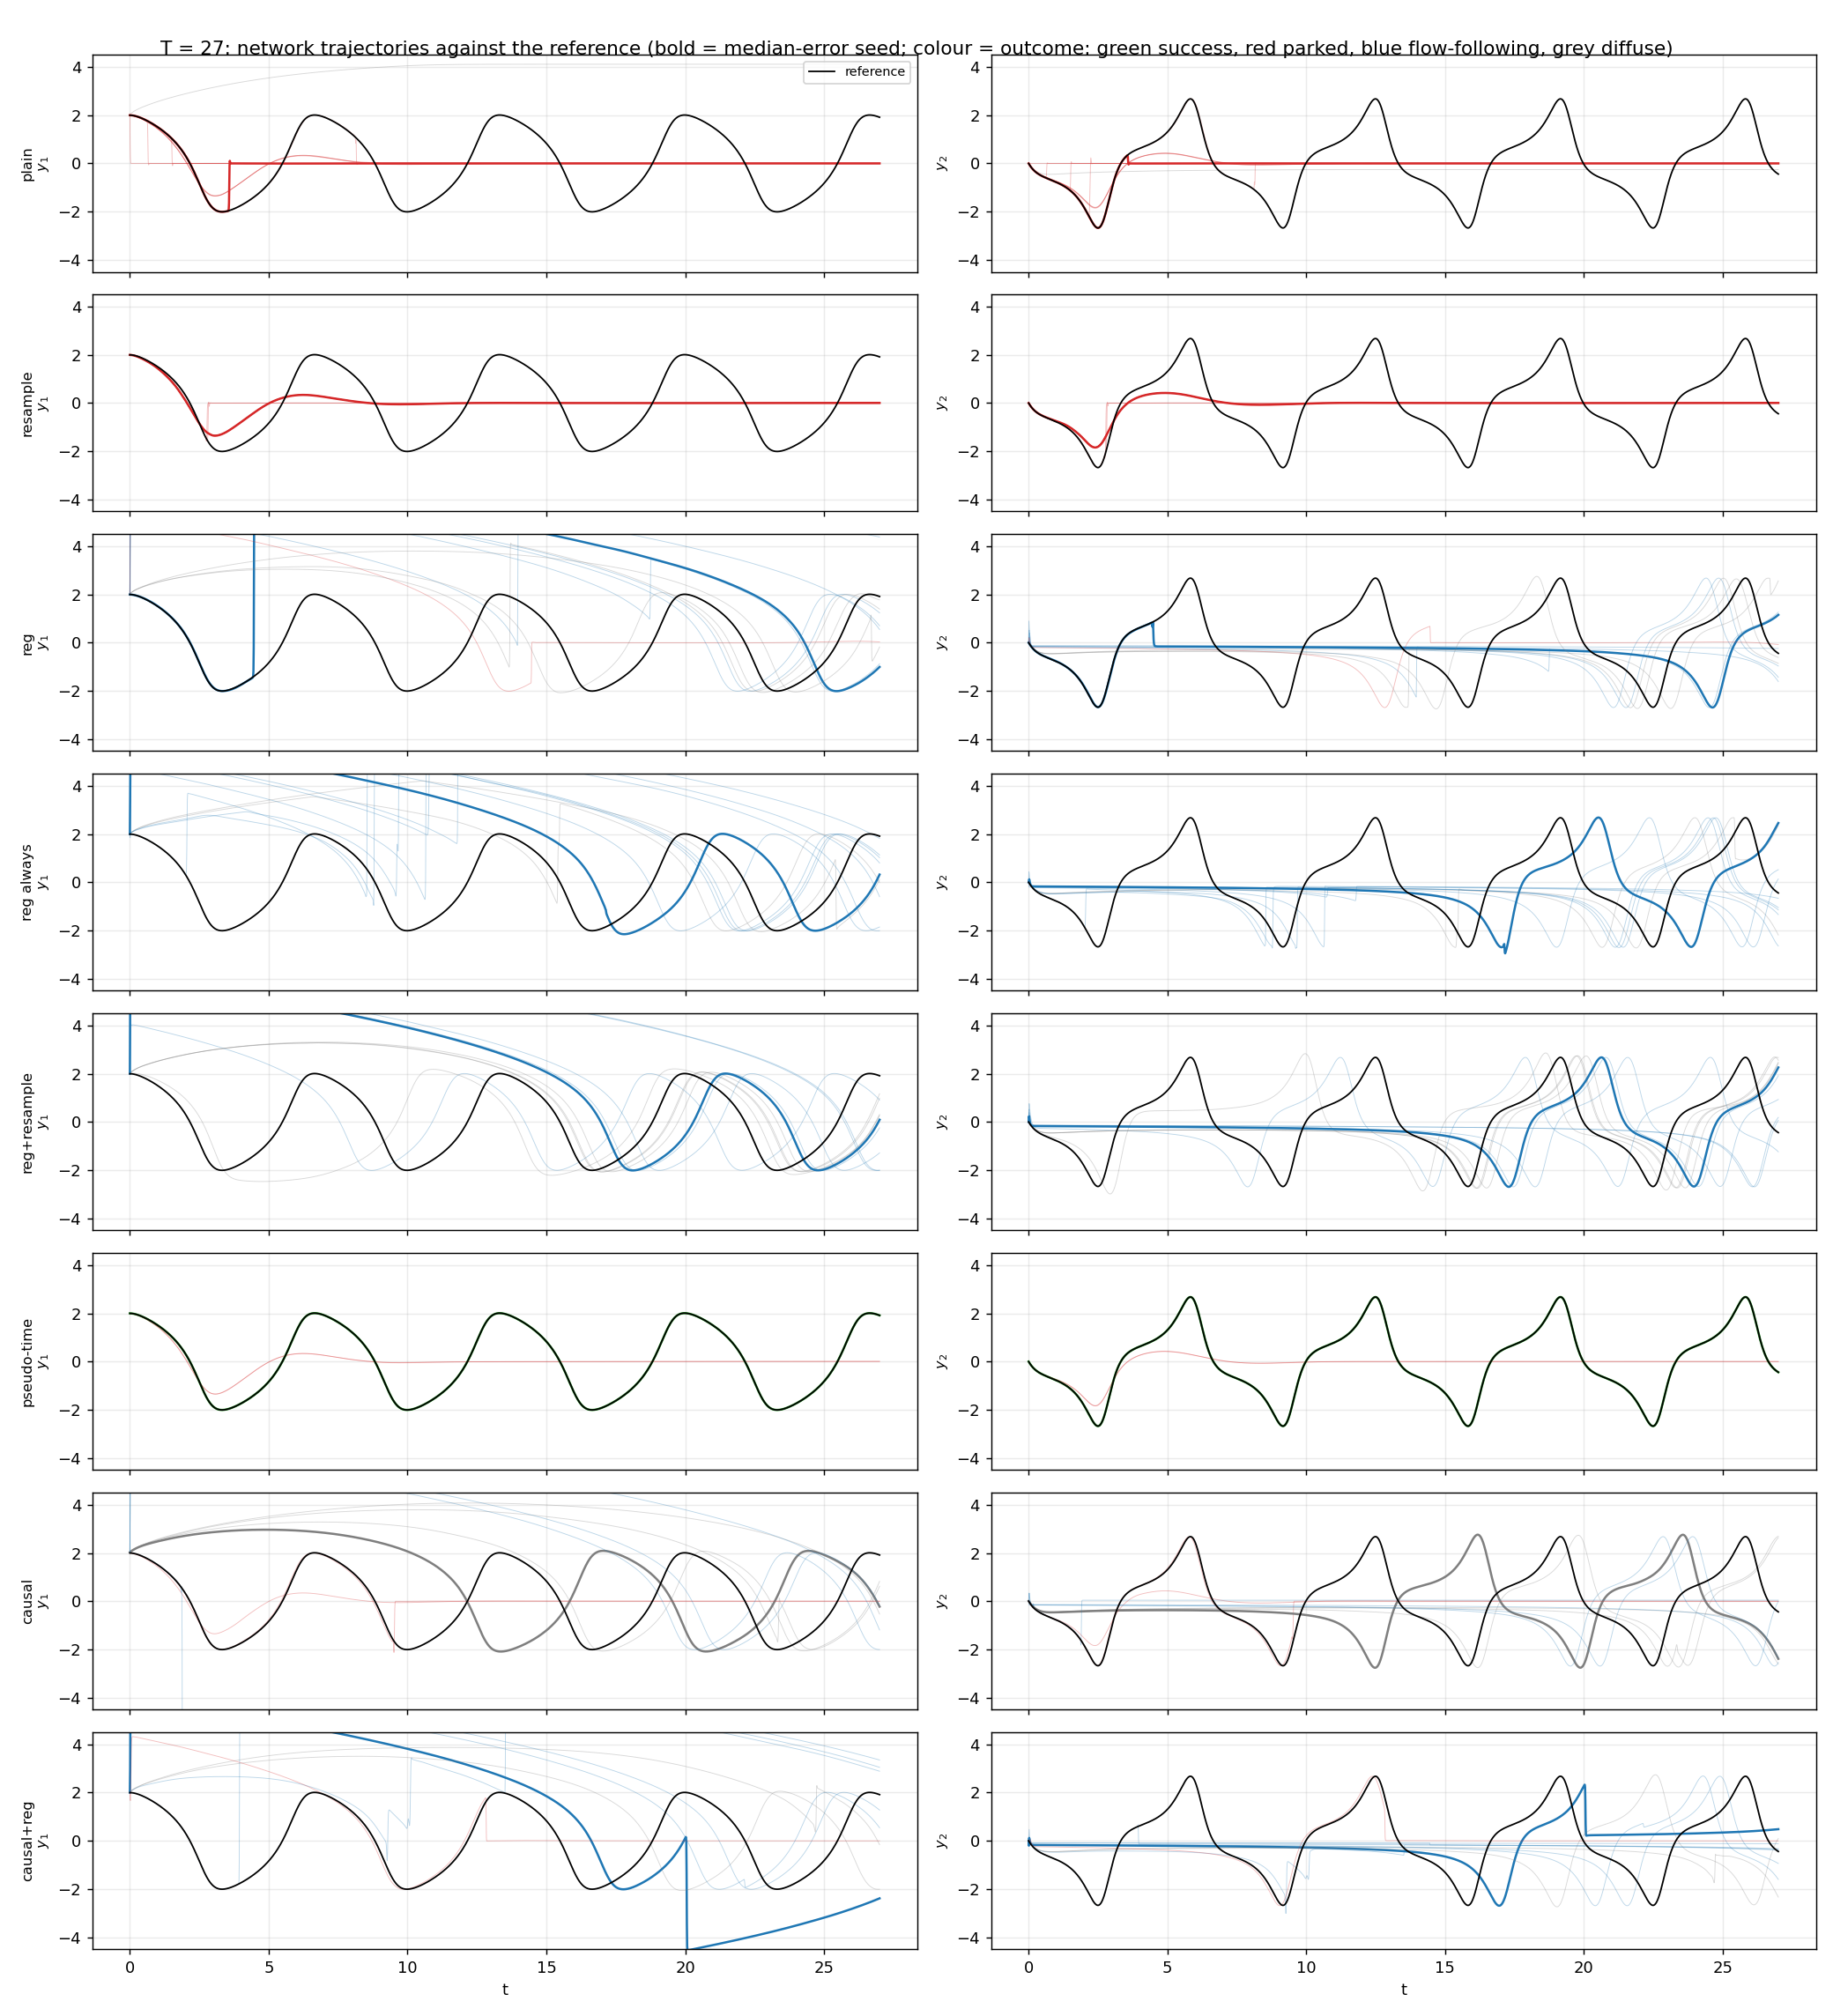
\includegraphics[width=\linewidth]{fig_arms_traj_T27.png}
  \caption{$T = 27$, both state components against time, every seed
  faint and the median-error seed bold, coloured by outcome (green
  success, red parked, blue flow-following, grey diffuse). The plain
  and resampled objectives follow the reference for about one period
  and stop at the origin; every regulariser variant leaves through the
  top of the frame at $t = 0$ and rides an off-loop trajectory back onto
  the cycle out of phase; pseudo-time stepping sits on the reference for
  the whole window.}
  \label{fig:arms-traj}
\end{figure}

\begin{figure}[tbp]
  \centering
  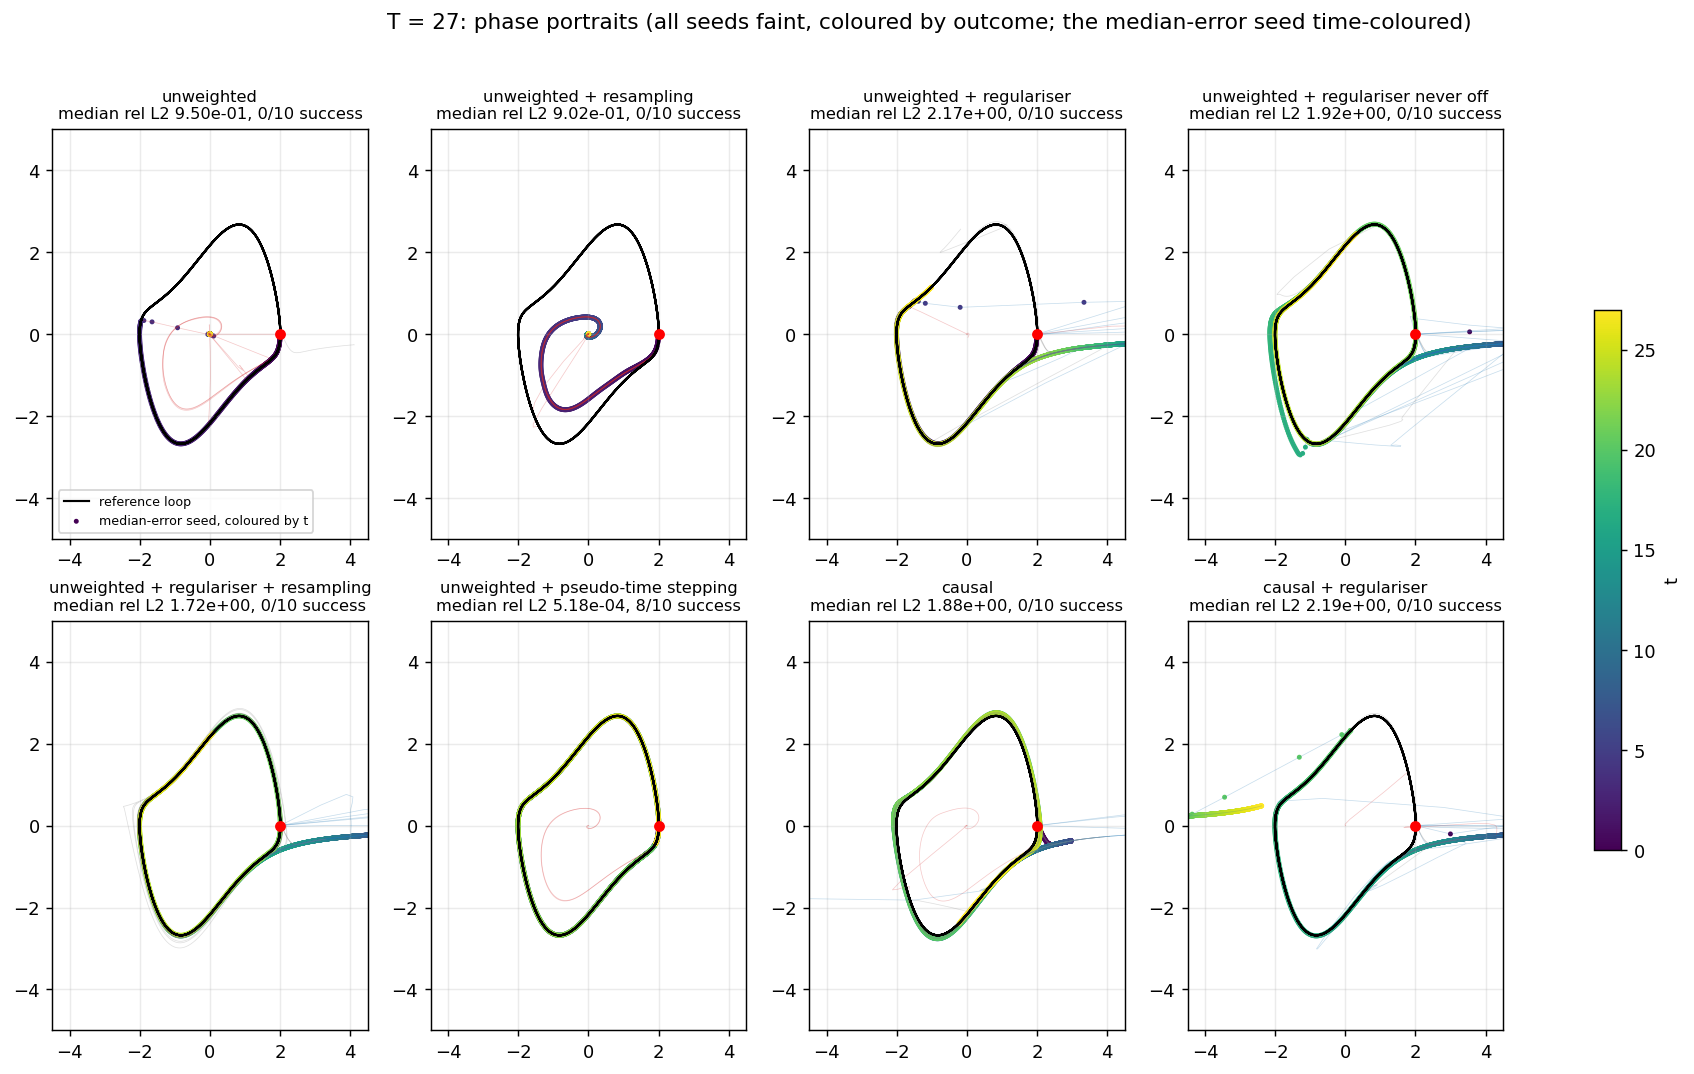
\includegraphics[width=\linewidth]{fig_arms_phase_T27.png}
  \caption{The same runs in the phase plane, the median-error seed
  coloured by time. The plain and resampled fits spiral into the origin;
  the regulariser variants enter from the right at $y_1 \approx 4.5$,
  far outside the cycle, and join the loop; pseudo-time stepping draws
  the loop itself. Several regularised fits sit on the loop and are
  still wrong in time.}
  \label{fig:arms-phase}
\end{figure}

\begin{figure}[tbp]
  \centering
  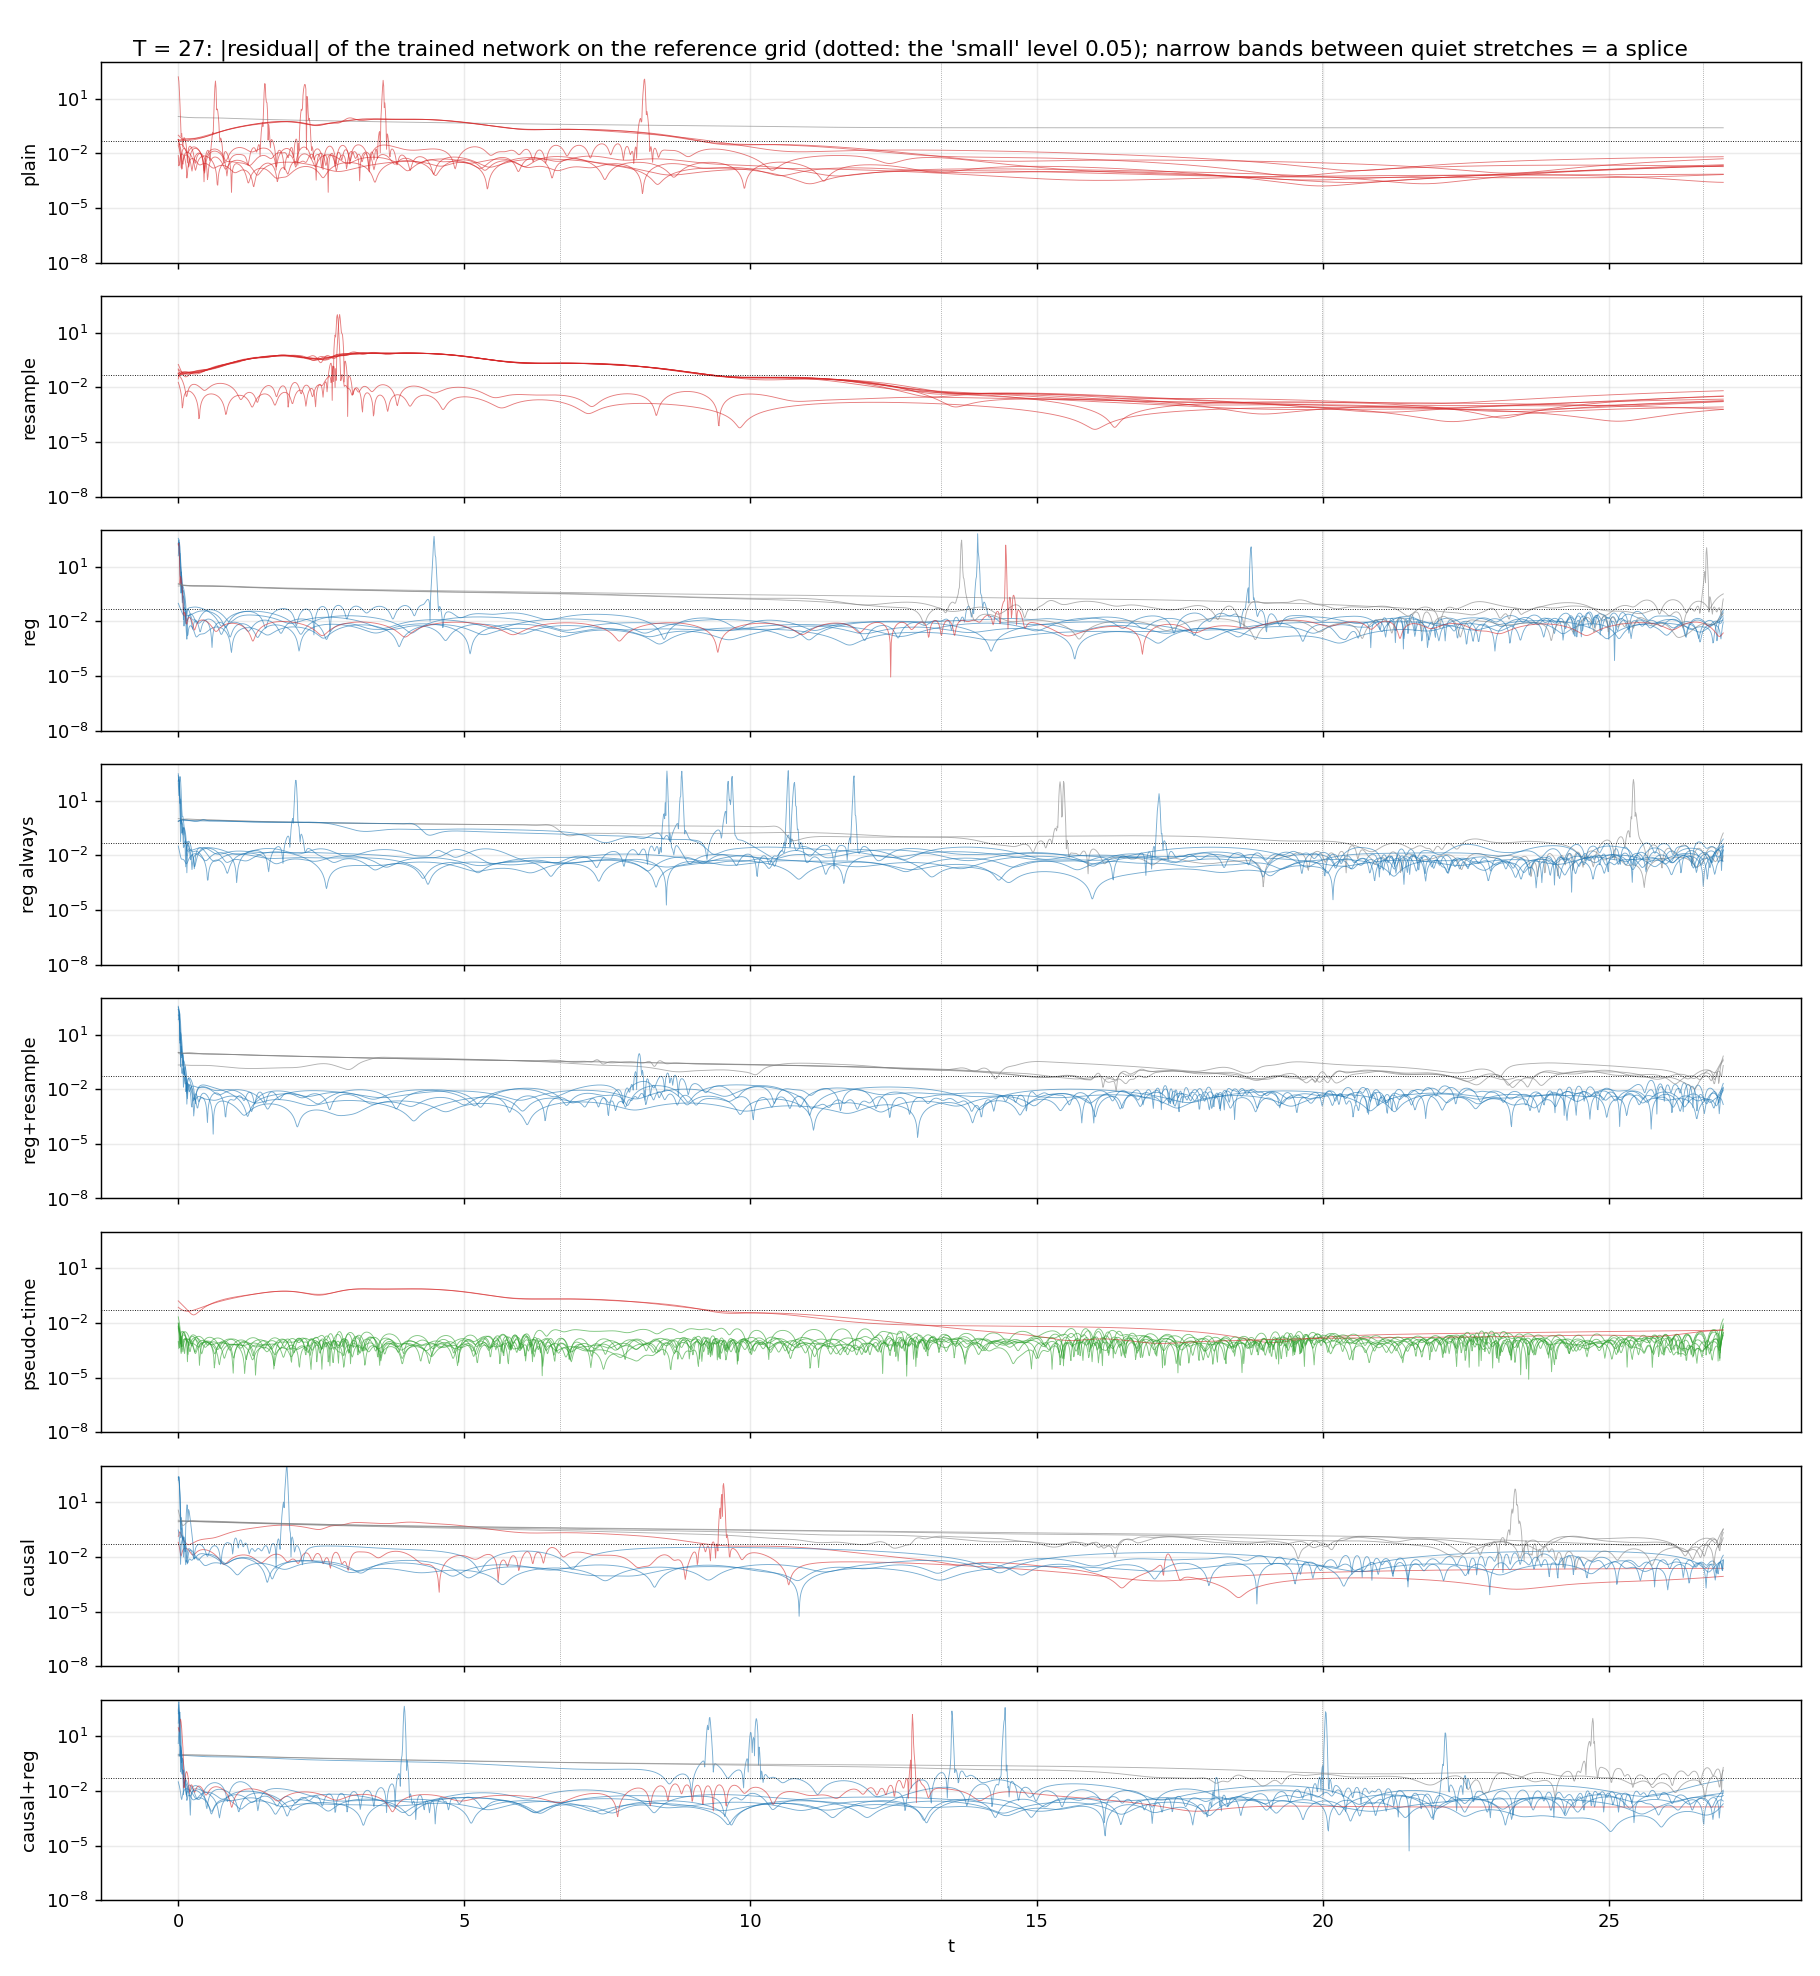
\includegraphics[width=\linewidth]{fig_arms_residual_T27.png}
  \caption{Where the residual is paid at $T = 27$: the absolute residual
  of the trained network on the reference grid, every seed, dotted line
  at $0.05$. Parks show a moderate residual across the hand-over and
  then quiet; every regulariser variant shows a residual below $0.05$
  almost everywhere with one spike right after $t = 0$, a splice placed
  in the first unsampled gap; pseudo-time successes show a flat residual
  near $10^{-3}$.}
  \label{fig:arms-residual}
\end{figure}

\begin{figure}[tbp]
  \centering
  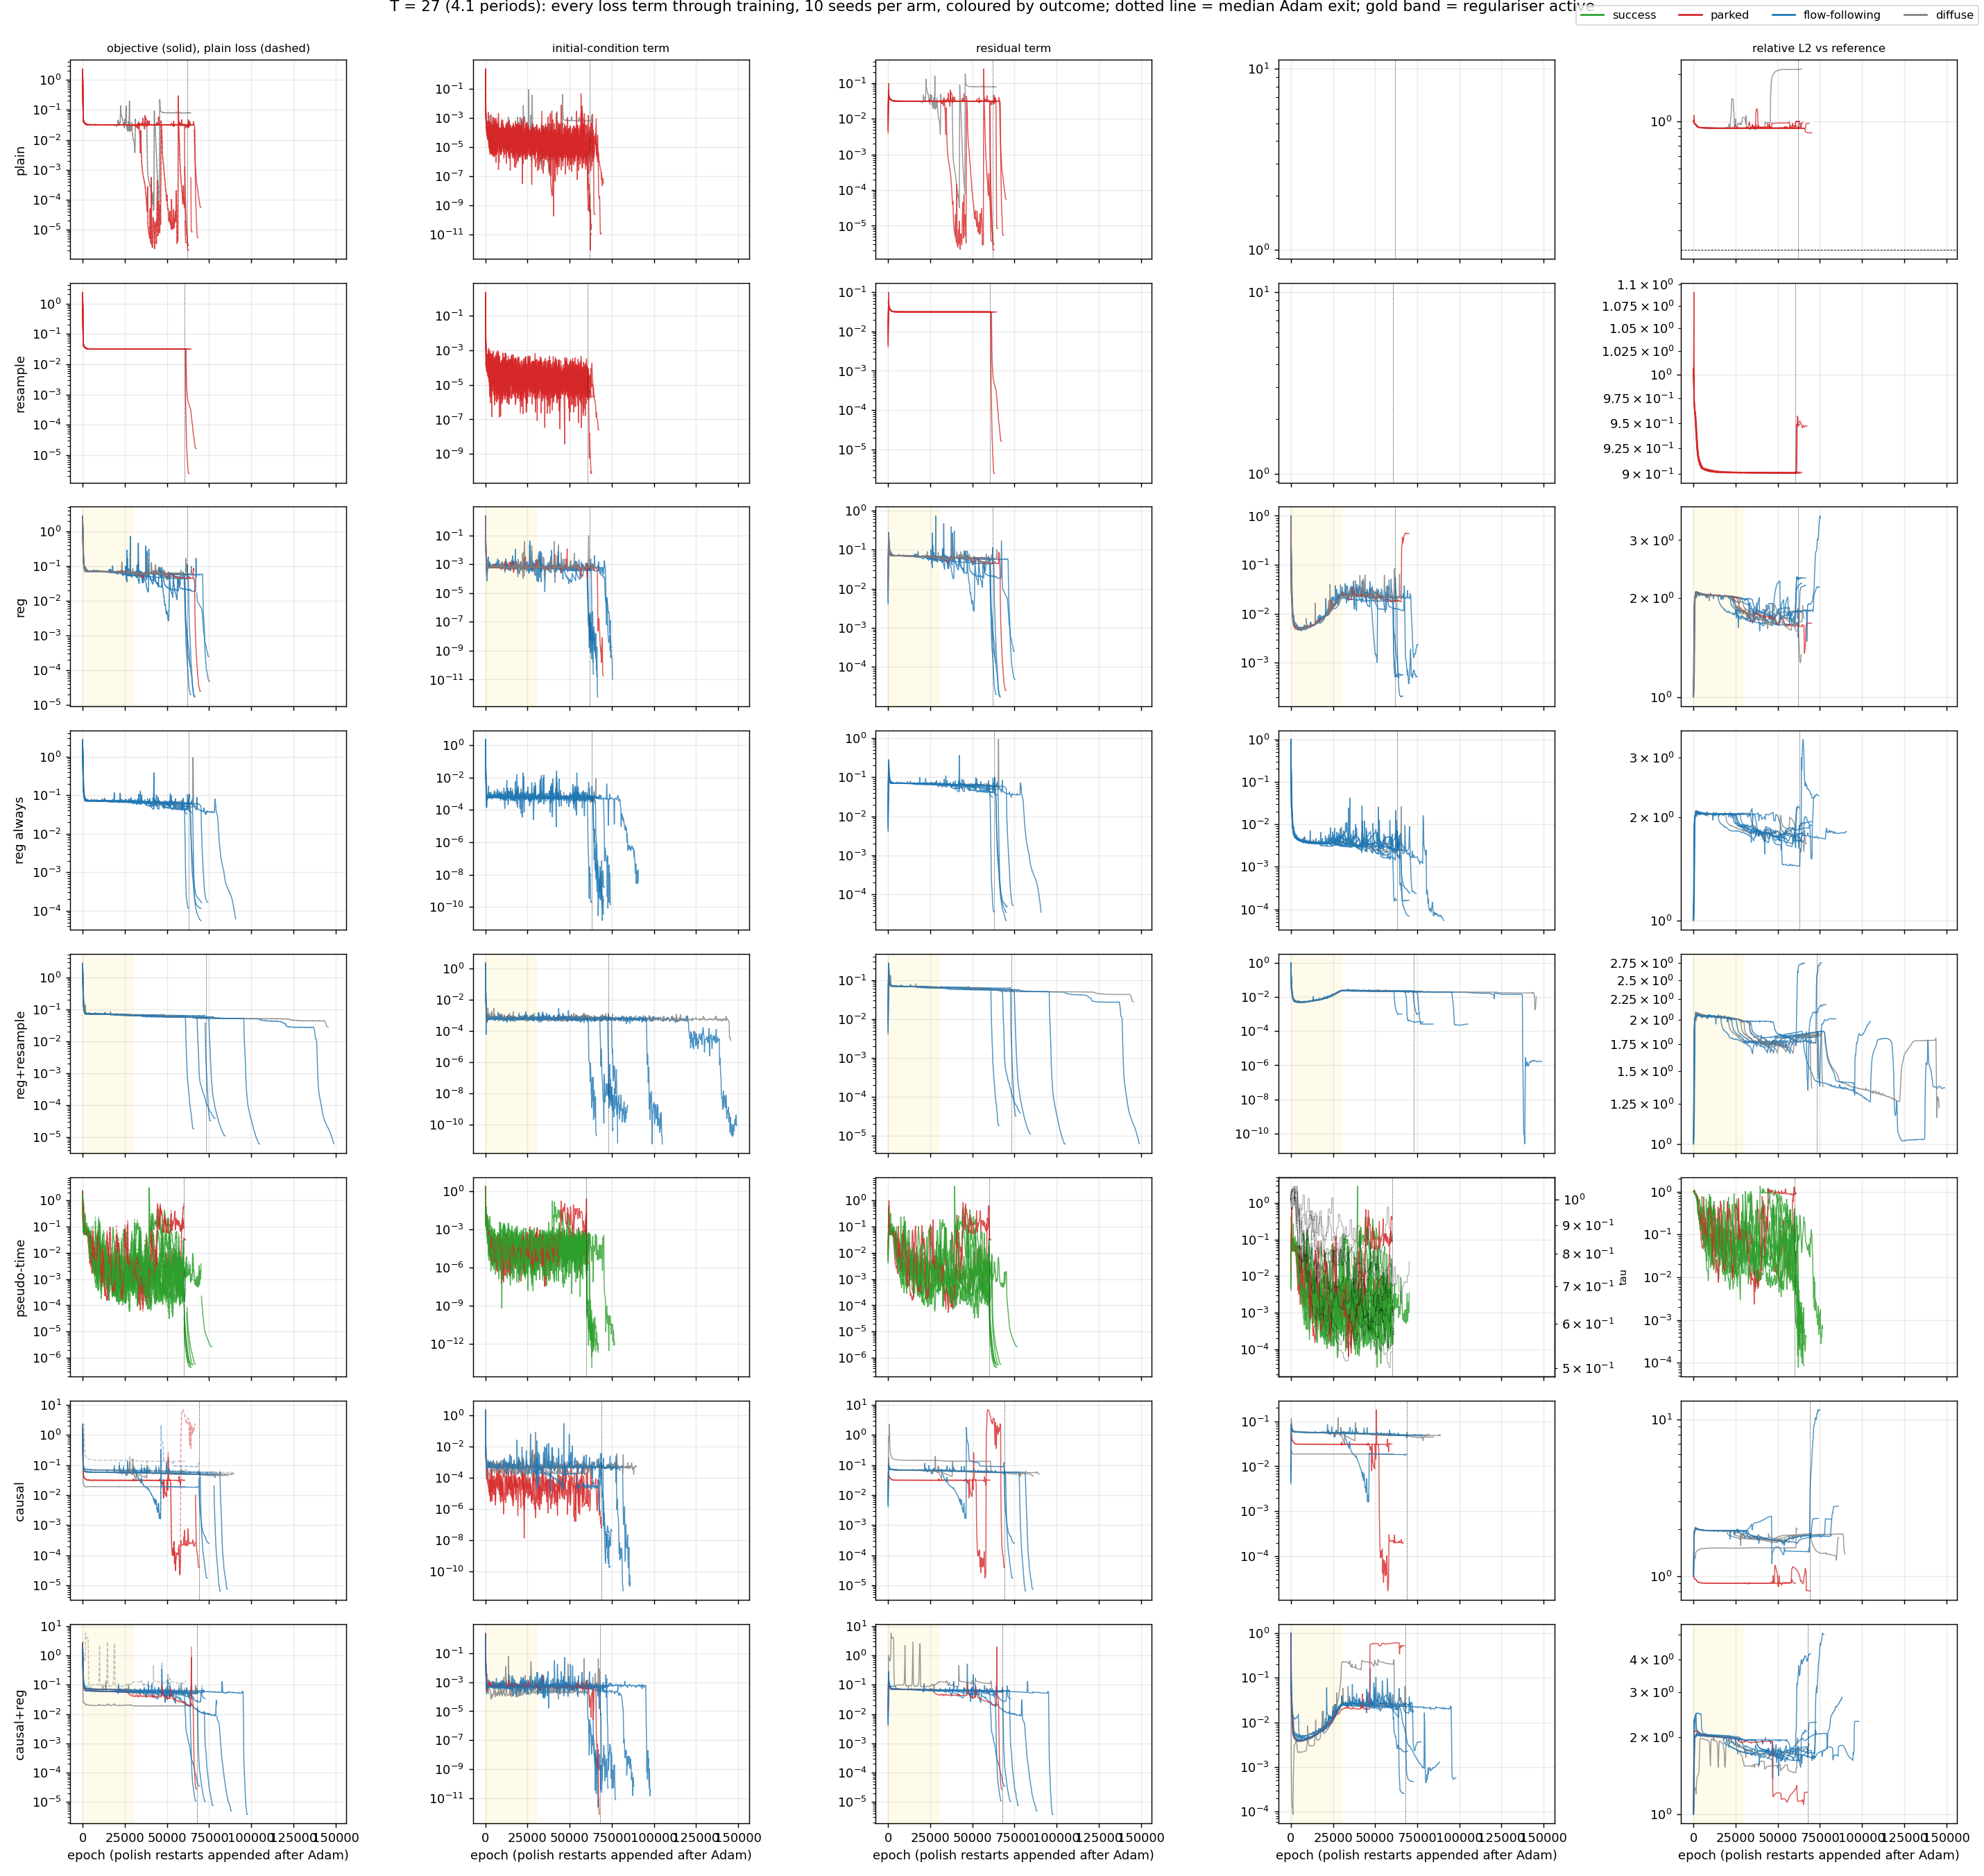
\includegraphics[width=\linewidth]{fig_arms_lossterms_T27.png}
  \caption{Every loss term through training at $T = 27$: objective,
  initial-condition term, residual term, the arm's own extra term and
  the relative $L_2$, every seed, Adam then the polish restarts. The
  parked plain runs reach the same objective as a success; in the
  regularised arms the regulariser value rises after switch-off while
  the objective falls; the polish lowers the flow-following objectives
  below $10^{-4}$ without moving the error.}
  \label{fig:arms-lossterms}
\end{figure}

\subsection{Density and horizon for pseudo-time stepping}
\label{sec:axes}

With one fix working, I measured how it responds to the two resources
a practitioner would reach for, with the plain objective as the
baseline and the regulariser plus resampling as the published control,
same protocol, seeds 0 to 9: collocation densities of 80 and 320 points
per unit time on top of 20 at $T = 14, 27, 40$, and horizons of $T = 67$
and $100$ (ten and fifteen periods) at density 20; 240 runs.

\begin{table}[tbp]
  \centering
  \caption{Successes out of ten against collocation density (left) and
  horizon at density 20 (right). The density-20 column and the
  $T \le 40$ entries are the runs of Table~\ref{tab:arms}.}
  \label{tab:axes}
  \small
  \begin{tabular}{lccc@{\hskip 2em}ccccc}
    \toprule
    & \multicolumn{3}{c}{density, $T=27$ / $T=40$} & \multicolumn{5}{c}{horizon, $T$} \\
    arm & 20 & 80 & 320 & 14 & 27 & 40 & 67 & 100 \\
    \midrule
    pseudo-time stepping & 8 / 7 & 9 / 5 & 10 / 8 & 10 & 8 & 7 & 1 & 0 \\
    plain & 0 / 0 & 0 / 0 & 0 / 0 & 5 & 0 & 0 & 0 & 0 \\
    regulariser + resampling & 0 / 0 & 3 / 0 & 0 / 0 & 10 & 0 & 0 & 0 & 0 \\
    \bottomrule
  \end{tabular}
\end{table}

\begin{figure}[tbp]
  \centering
  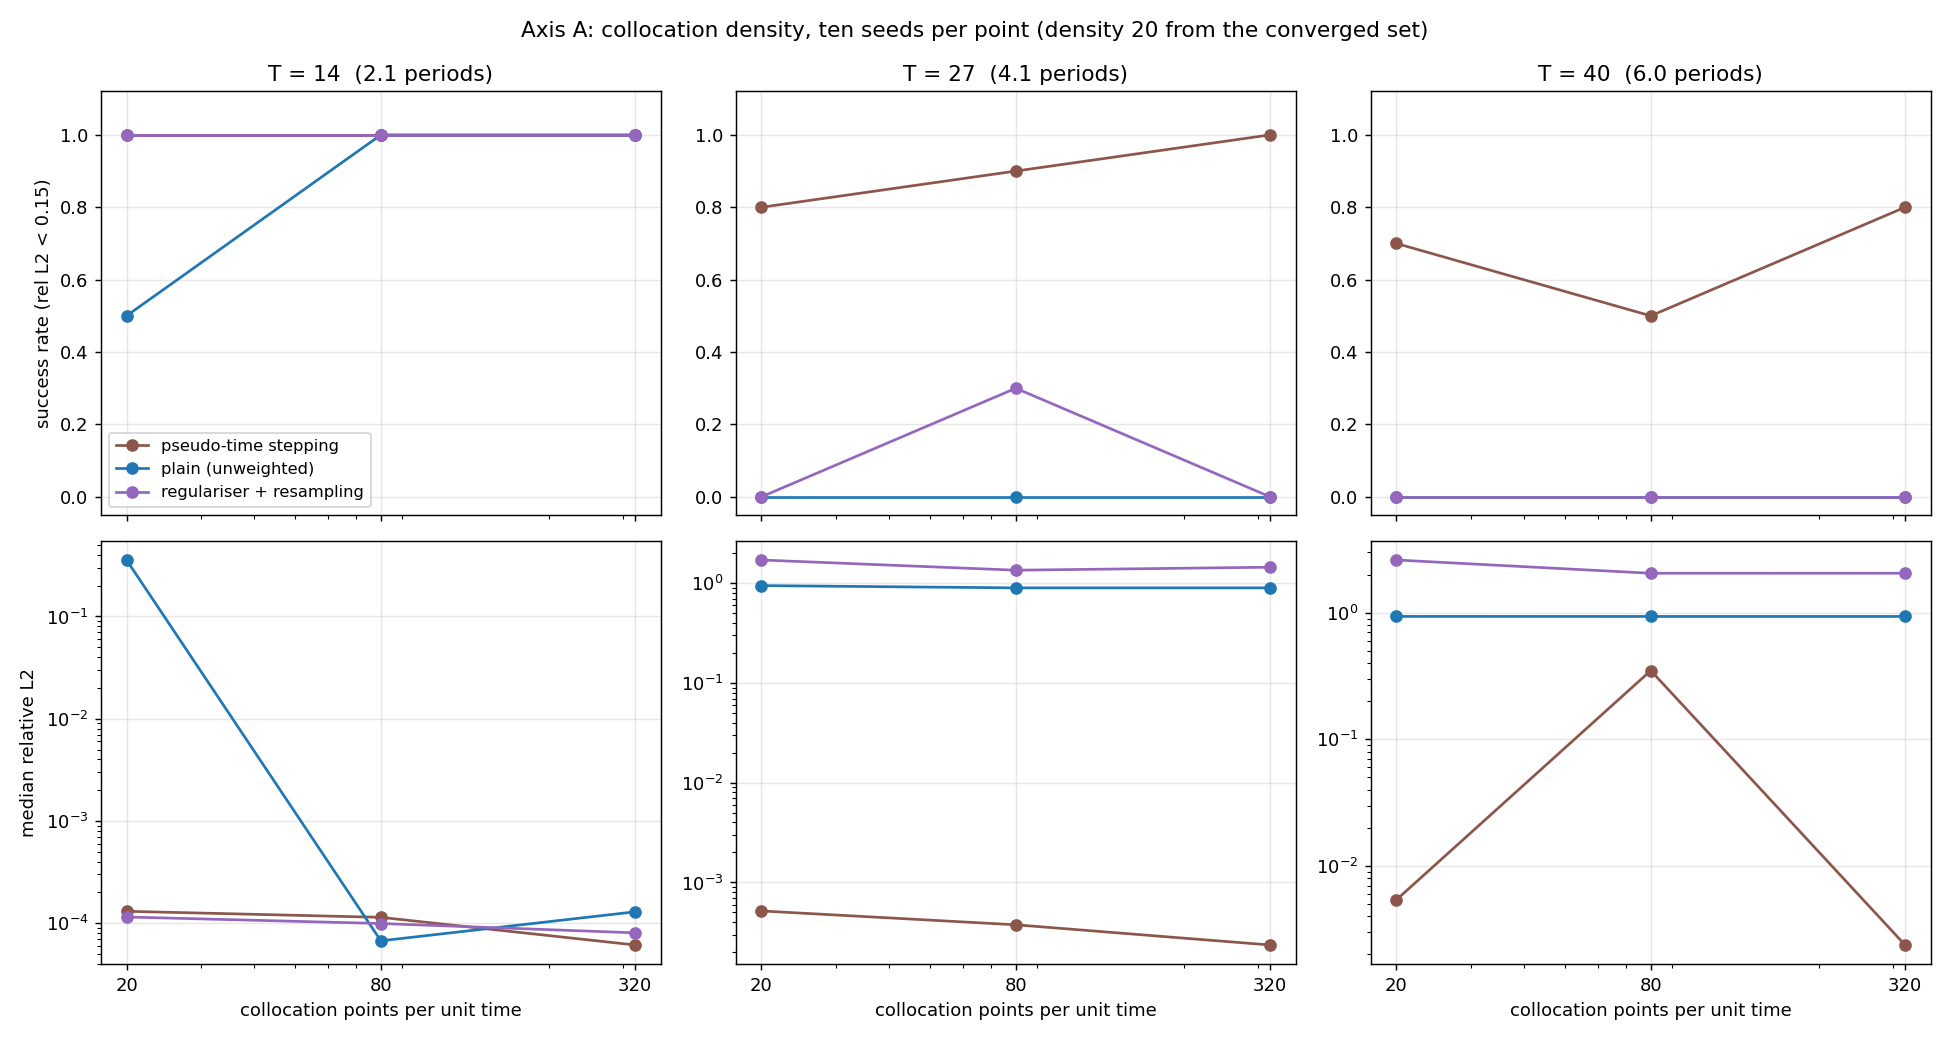
\includegraphics[width=\linewidth]{fig_axes_density.png}
  \caption{Success rate (top) and median relative $L_2$ (bottom)
  against collocation density, one column per horizon, ten seeds per
  point.}
  \label{fig:axes-density}
\end{figure}

\begin{figure}[tbp]
  \centering
  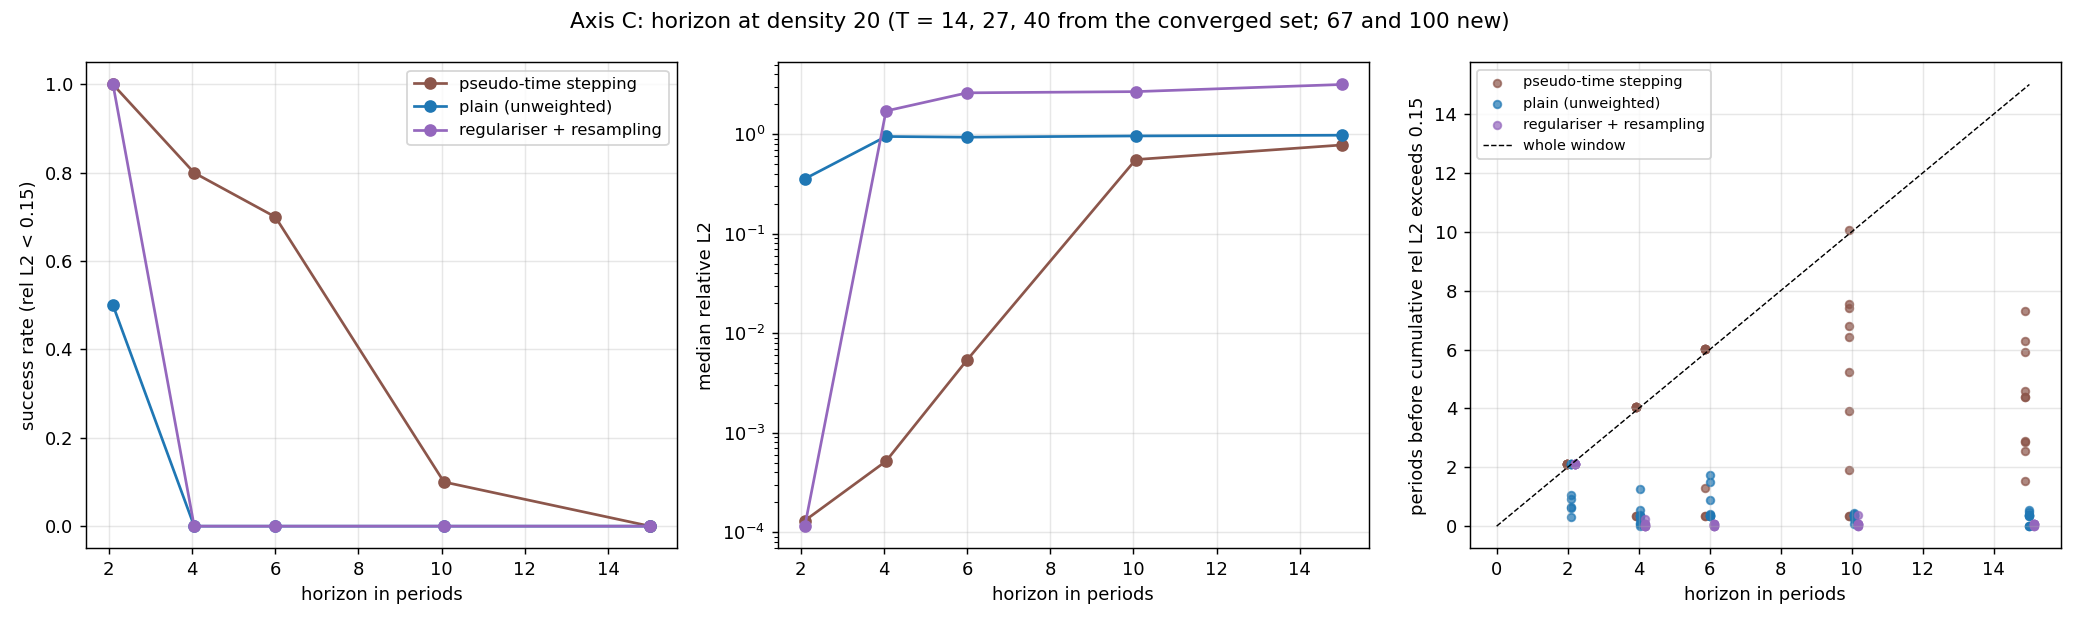
\includegraphics[width=\linewidth]{fig_axes_horizon.png}
  \caption{Success (left), median relative $L_2$ (middle) and the number
  of periods survived before the cumulative relative $L_2$ exceeds
  $0.15$ (right), per run, against the horizon in periods.}
  \label{fig:axes-horizon}
\end{figure}

\begin{figure}[tbp]
  \centering
  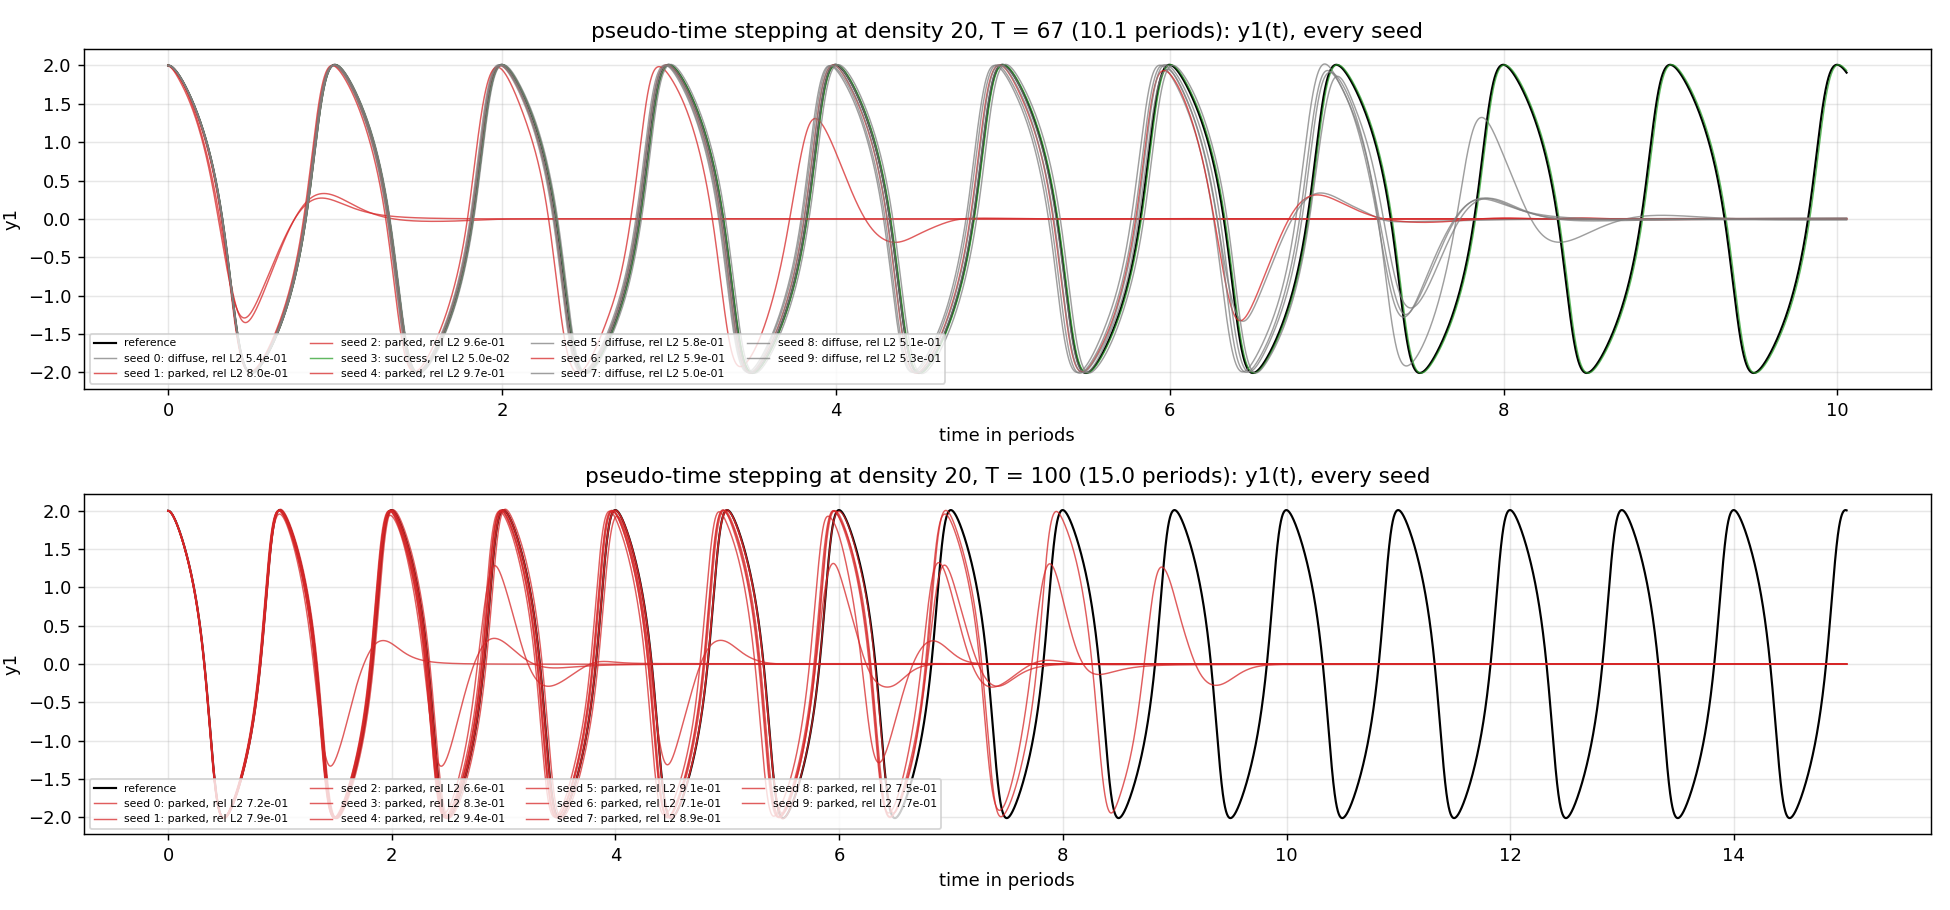
\includegraphics[width=\linewidth]{fig_axes_long_horizon.png}
  \caption{Pseudo-time stepping at $T = 67$ and $T = 100$, $y_1$
  against time in periods for every seed, coloured by class. The
  failures are late parks: the network rides the loop for four to eight
  periods, drifts off, and sits at the origin. Nothing wanders off the
  loop.}
  \label{fig:axes-long}
\end{figure}

\begin{figure}[tbp]
  \centering
  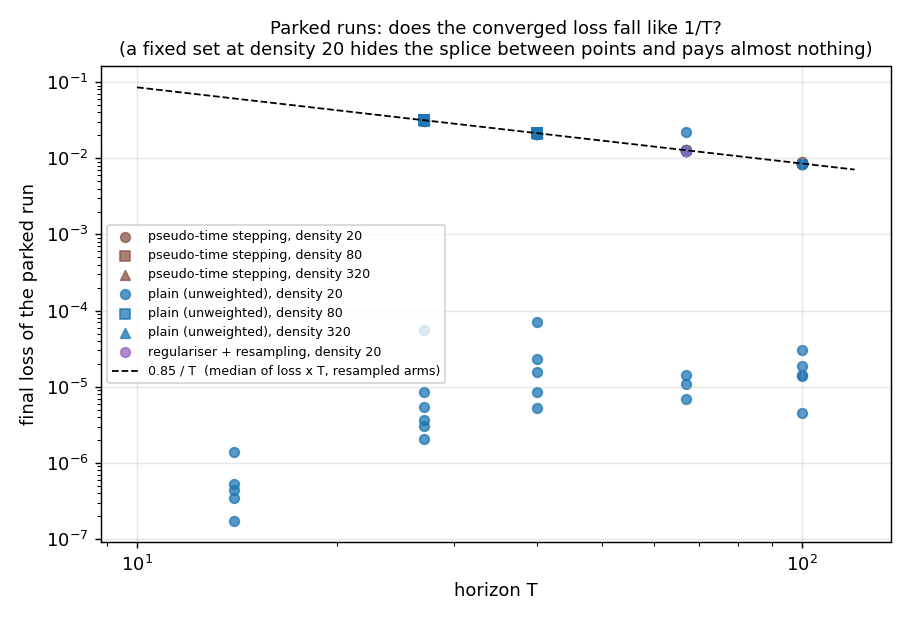
\includegraphics[width=0.75\linewidth]{fig_axes_parked_loss.png}
  \caption{The converged loss of every parked run against $T$, with
  the $1/T$ line through the median of loss $\times T$ over the
  resampled arms. The resampled arms at every density, and the plain
  arm at densities 80 and 320, sit on the line from $T = 27$ to
  $T = 100$; the plain arm at density 20 sits three to four orders
  lower.}
  \label{fig:axes-parked}
\end{figure}

Three things move (Table~\ref{tab:axes}, Figure~\ref{fig:axes-density}).
At two periods, density 80 lifts the plain objective from 5 of 10 to
10 of 10, so the null verdict of Section~\ref{sec:density}, obtained at
a fixed budget with L-BFGS alone, does not survive training to
convergence; at four periods and beyond the plain objective still fails
at every density, so the verdict there stands. The published
regulariser protocol has its first successes past two periods at
density 80, 3 of 10 at four periods, one of them converged and two
budget-limited, with the other seven diffuse; at density 320 it is back
to 0 of 10. And pseudo-time stepping's parking rate at four periods
falls with density, 8, 9 and 10 of 10, while at six periods it does not
move in any direction, 7, 5 and 8 of 10, with different seeds parking
at each density and every parked run sitting at the same loss whatever
the density. Ten seeds cannot separate the six-period rates.

On the horizon axis (Figures~\ref{fig:axes-horizon}
and~\ref{fig:axes-long}), pseudo-time stepping's own wall at density 20
lies between six and ten periods: 7 of 10 at six, 1 of 10 at ten (a
marginal success at $5\times10^{-2}$ with the polish at its cap), 0 of
10 at fifteen. The failure mode does not change with the horizon, it
arrives later: the parked branch after four to eight good periods.

Figure~\ref{fig:axes-parked} tests the price of Eq.~\eqref{eq:layerprice}
directly. Over the 65 parked runs whose transition layer is actually
sampled, the resampled arms at any density and the plain arm at
densities 80 and 320, loss $\times T$ has median $0.85$ and ranges
$0.84$ to $0.90$, from $T = 27$ to $100$. The plain arm's parked runs at
density 20 sit three to four orders of magnitude lower, because a fixed
set of 20 points per unit time leaves room to hide the layer; at
density 80 the gap is too small to hide in and a fixed set behaves like
resampling. Two consequences follow. The $1/T$ prediction holds
quantitatively. And more density cannot move a resampled method's wall
by pricing: the parked branch is already fully sampled, so denser points
do not raise its price. What density can do is make the descent to the
truth cheaper than the descent to the park in more seeds, which is what
the four-period column shows and the six-period column does not. Cost
grows roughly linearly with the number of collocation points; the
density-320 runs at $T = 40$, with 12,800 points, took about four hours
each, the most expensive in this chapter.

Four issues remain open. Density is not a lever past four periods and
multiplies the cost. The wall between six and ten periods is a late
park, and what sets its position, the $\tau$ schedule, the anchor's
fading influence or the $1/T$ price finally undercutting the truth, is
not yet measured. The failure classifier reads late parks as diffuse,
so the periods-survived readout of Figure~\ref{fig:axes-horizon} is the
right one for long windows. And the regulariser protocol's three
successes at density 80 are mostly budget-limited and should be
extended before they are counted.

\subsection{What the continuous-time route establishes}
\label{sec:cont-summary}

The continuous-time formulation works, per starting state, up to a horizon that no resource moves. It reproduces the source work's accuracy below one period; causal weighting, the strongest loss-level modification in the literature, moves the failure from one period out to two and makes it visible in the training telemetry; and beyond that, optimisation budget ($4\times$, none of seven), network size (600 runs, depth harmful), collocation density (64-fold range) and collocation placement all leave the outcome unchanged under the original protocol. The one variable that orders those outcomes is the starting state: success at two periods occurs in 19 of 150 causally weighted runs at the 1\% threshold and depends on where the start sits, and at four periods none of the 300 runs of either variant succeeds. The failure study then says why. The same networks fit four periods from data, so the objective is at fault; the objective is exactly satisfied by a whole family of spliced trajectories of which the fixed point is the cheapest, at a price that falls like $1/T$ under resampling and is measured to do so; the published fixed-point regulariser closes the origin and the optimiser takes the next member of the family; and the one objective that prices the whole family, pseudo-time stepping with resampling, carries the formulation from two periods to six, with its own wall between six and ten and no help from collocation density. Taken together, these findings say that the continuous-time formulation fails through what its objective accepts, that the fix must act on the objective rather than on any resource, and that even the best such fix runs out within ten periods; they motivate imposing the physics structurally instead, which is the discrete-time formulation of the next section.

% ===========================================================================
\section{The discrete-time formulation}
\label{sec:disc-method}

\subsection{Implicit Runge--Kutta background}

Integrating $\dot y = f(y)$ exactly across one step gives
\begin{equation}
  y(t + \Delta t) = y(t) + \int_t^{t+\Delta t} f\big(y(s)\big)\, ds ,
  \label{eq:step-integral}
\end{equation}
so a one-step numerical method is, at heart, a quadrature rule (a recipe
for approximating an integral from a few point evaluations) applied to
Eq.~\eqref{eq:step-integral}. The simplest choice, approximating the
integrand by its value at the left endpoint, is Euler's method,
$y^{n+1} = y^n + \Delta t\, f(y^n)$. Better quadrature needs the
integrand at interior times of the step; but the integrand is
$f(y(s))$, and $y(s)$ is exactly what is not yet known there. The
Runge--Kutta family resolves this circularity by introducing $q$
\emph{stage states}, internal estimates of the solution at chosen
fractions $c_1, \dots, c_q$ of the step, defined self-consistently
through each other:
\begin{equation}
  y^{n+c_j} = y^n + \Delta t \sum_{k=1}^{q} a_{jk}\, f\big(y^{n+c_k}\big),
  \qquad
  y^{n+1} = y^n + \Delta t \sum_{j=1}^{q} b_j\, f\big(y^{n+c_j}\big),
  \label{eq:irk}
\end{equation}
where $y^{n+c_j}$ denotes the stage state at time $t_n + c_j\,\Delta t$,
and the nodes $c$, matrix $A = (a_{jk})$ and weights $b$ form the Butcher
tableau, which specifies the method completely. If $A$ is strictly
lower triangular, each stage depends only on earlier ones and the step is
computed left to right: an explicit method (the sixth-order reference
integrator of Section~\ref{sec:problem} is one). When $A$ is full, every
stage depends on every other and the first relation of
Eq.~\eqref{eq:irk} is a genuine coupled system of $2q$ nonlinear
equations (two state components times $q$ stages): the method is
implicit, normally solved by a root-finder at every step.

Why pay the implicit price? Two properties, and both matter here.
\begin{itemize}
  \item \textbf{Order.} A method has order $p$ if the error of one step
  shrinks like $\Delta t^{p+1}$, so that the accumulated error over a
  fixed interval shrinks like $\Delta t^{p}$; halving the step of an
  order-6 method cuts the error 64-fold. Gauss--Legendre tableaus place
  the nodes $c_j$ at the roots of the degree-$q$ Legendre polynomial
  mapped to $[0,1]$, the same points that make Gaussian quadrature exact
  for polynomials of degree $2q-1$, and attain order $2q$, the maximum
  any $q$-stage method can achieve: each added stage buys two orders.
  \item \textbf{A-stability.} Stability is probed on the linear test
  equation $\dot y = \lambda y$ with $\mathrm{Re}\,\lambda < 0$, whose
  true solution decays; a method is A-stable if its numerical solution
  also decays at every step size. Explicit methods never are (too large
  a step and the numerical solution explodes although the true one
  decays), while Gauss--Legendre methods are A-stable at every
  order~\cite{hairer1996}. A-stability is, however, a \emph{linear}
  property: on a nonlinear system the implicit stage equations must also
  have a findable solution, and that solvability, not stability, is
  what breaks first as the step grows (measured directly in
  Section~\ref{sec:disc-routes}).
\end{itemize}
Gauss--Legendre methods are also collocation
methods in the classical sense: there is a single
degree-$q$ polynomial through $y^n$ that satisfies the differential
equation exactly at the $q$ node times, and the stages are its values
there, so the stage states approximate the solution at the interior
times $c_j\,\Delta t$ to high order. They are not abstract
intermediates (Figure~\ref{fig:anatomy}).

\begin{figure}[tbp]
  \centering
  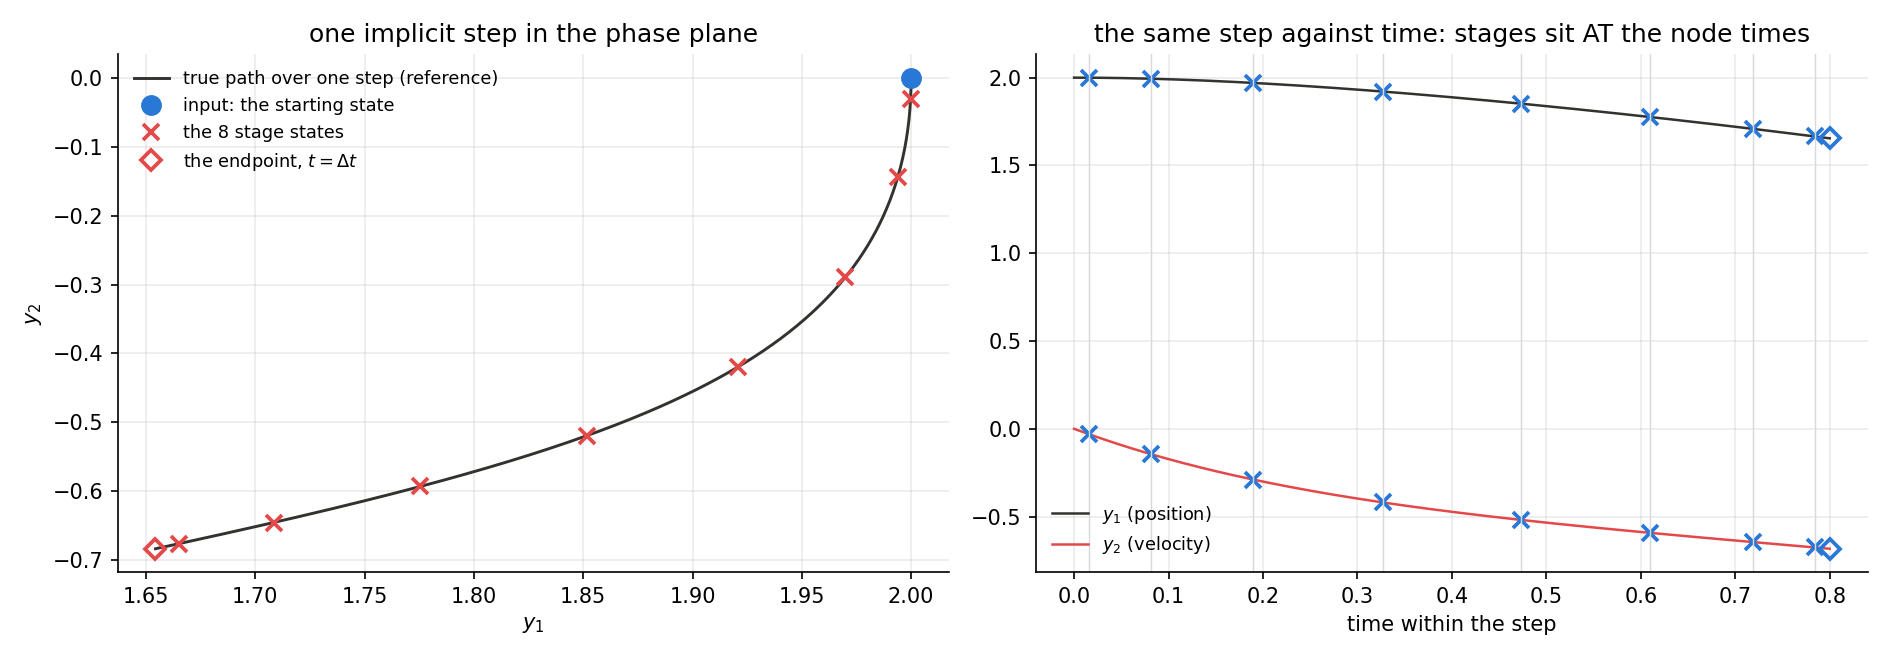
\includegraphics[width=0.8\linewidth]{fig_step_anatomy.png}
  \caption{Anatomy of one implicit step from $(2,0)$ at $q=8$: the true
  path over $[0, 0.8]$, the eight Gauss stage states (exact solver), and
  the endpoint. The stages lie on the true mini-trajectory, crowding toward
  the ends of the step where the Legendre roots sit. Given the input state,
  the network must place all nine points.}
  \label{fig:anatomy}
\end{figure}

\subsection{The loss}

The source work's discrete-time construction replaces the root-finding
solve of Eq.~\eqref{eq:irk} by a network that proposes all $q+1$ unknowns
at once; each defining relation is rearranged to isolate the known state,
\begin{equation}
  \underbrace{y^{n+c_j} - \Delta t \sum_k a_{jk} f\big(y^{n+c_k}\big)}_{\text{reconstruction } j} = y^n
  \qquad\text{and}\qquad
  \underbrace{y^{n+1} - \Delta t \sum_j b_j f\big(y^{n+c_j}\big)}_{\text{reconstruction } q+1} = y^n ,
  \label{eq:recon}
\end{equation}
so that if the network's outputs really are the stage states of the scheme,
all $q+1$ reconstructions land exactly on $y^n$. The loss I use is the
mean of the squared reconstruction mismatches over outputs, components and
batch.
(In the source work the loss is a sum rather than a mean and carries an
additional boundary term; for an ordinary differential equation there is no
boundary, and at fixed batch size the mean is a rescaled sum. Both
differences are noted for exactness.) Nothing else is supervised: there is
no time derivative of the network, no collocation grid over time, and no
trajectory data. The tableau is fixed and known; only the stage values are
learned. The anchoring that the continuous-time formulation concentrates
in a single point is here built into every term of the loss: every output
is tied to a known state through the algebra of the step.

\subsection{The state as the input: a reusable one-step map}

In the source work the network input is a spatial coordinate and the known
$y^n$ is a measured snapshot of a field; an ordinary differential equation
has no spatial coordinate, so the input becomes \emph{the starting state
itself}: the network maps $(y_1, y_2)$ to the $q$ stage states plus the
endpoint, $2(q+1)$ numbers. Trained over a region of starting states, one
network becomes a reusable map for the fixed step: feed in any state
and receive the state $\Delta t = 0.8$ later; feed the endpoint back in
and a whole trajectory follows, without retraining. The step size 0.8 is
taken from the source work's own demonstration, so the comparison
inherits its setting; no other value is tested here, a limitation
Section~\ref{sec:future} takes up. This construction differs from the
sequential mode described in the source work, which retrains at every
step. The generalisation itself follows Fern\'andez Corral et
al.~\cite{fernandez2024}, who apply it to conservative and periodically
forced systems; the dissipative limit-cycle instantiation, the
exact-scheme error attribution, the seed and selection analysis, and the
head-to-head comparison with the continuous-time formulation below are, to
my knowledge, new.

\subsection{Protocol and guardrails}
\label{sec:guardrails}

I train on 2000 starting states per run, Latin-hypercube sampled over
the rectangle $y_1 \in [-2.5, 2.5]$, $y_2 \in [-3, 3]$, the limit cycle
with margin. The rectangle is a sampling region only; nothing constrains
a trajectory to remain inside it, unlike a boundary condition in a
partial differential equation. (This is the discrete-time
analogue of the collocation budget of Section~\ref{sec:collocation}: the
equations are enforced at 2000 points of the \emph{state space}, rather
than on a grid in time; Section~\ref{sec:baseline} varies this count and
finds the error flat from about 500 points.) The network body is
identical to the continuous-time experiments (4 hidden layers of 50
hyperbolic-tangent units, double precision) with a linear output layer
of $2(q+1)$ units; only the output layer grows with $q$. At $q = 8$ this
means 18 outputs and $8{,}718$ trainable parameters, and the interior
node times of the step are
$c_j\,\Delta t = \{0.016, 0.081, 0.190, 0.327, 0.473, 0.610, 0.719,
0.784\}$, the Gauss--Legendre nodes of
Section~\ref{sec:disc-method} scaled by $\Delta t = 0.8$. Each input
component is scaled by its half-range ($y_1$ by 2.5 and $y_2$ by
3), the discrete-time analogue of the declared time rescaling of
Section~\ref{sec:cont-method}. The optimiser, restart discipline and
epoch budget are identical to Section~\ref{sec:cont-protocol}, so
differences between the formulations are the formulation's. The sweep is
$q \in \{2, 4, 8, 16, 32\}$ times three seeds, fifteen runs.

Because the trained map will be judged against the scheme it imitates, the
scheme itself is verified first, independently of any network, in three
steps:
\begin{enumerate}
  \item the tableau is constructed for each $q$ from the Legendre roots
  and checked against every identity it must satisfy (row sums,
  quadrature exactness to degree $2q-1$, the collocation conditions, and
  a symplecticity identity that the construction never uses, which makes
  it an independent check); the worst violation up to $q = 32$ is
  $2\times10^{-16}$, machine precision;
  \item an exact solver (a root-finder on the $2q$ stage equations,
  convergence judged on the residual itself) then provides the scheme
  with no network in it, and its measured convergence order on problems
  with known solutions matches or exceeds the theoretical $2q$; and
  \item a single step of $0.8$ from 100 sampled states converged in 100
  of 100 cases at every $q$, establishing that the step is well-posed on
  the whole training region.
\end{enumerate}
Evaluation is on a held-out $21\times21$ uniform grid over
the rectangle (441 states, disjoint from the training samples by
construction, with the origin at its centre) and, for chained evaluation,
on a held-out test set of 108 starting states; all ground truths are
regenerated by the reference integrator, stopping exactly at each stage
time.

\subsection{Results: the error floor}
\label{sec:disc-results}

\begin{table}[tbp]
  \centering
  \caption{Endpoint relative $L_2$ error on the 441 held-out states versus
  the number of stages $q$ (median over three seeds), against the exactly
  solved scheme on the same states and metric.}
  \label{tab:floor}
  \small
  \begin{tabular}{ccc}
    \toprule
    $q$ (order $2q$) & trained network (median) & exact scheme, same grid \\
    \midrule
    2 (4)   & $3.94\times10^{-2}$ & $4.20\times10^{-2}$ \\
    4 (8)   & $4.57\times10^{-3}$ & $2.20\times10^{-4}$ \\
    8 (16)  & $3.61\times10^{-3}$ & $2.38\times10^{-8}$ \\
    16 (32) & $3.63\times10^{-3}$ & $8.9\times10^{-14}$ \\
    32 (64) & $3.63\times10^{-3}$ & $1.4\times10^{-13}$ \\
    \bottomrule
  \end{tabular}
\end{table}

\begin{figure}[tbp]
  \centering
  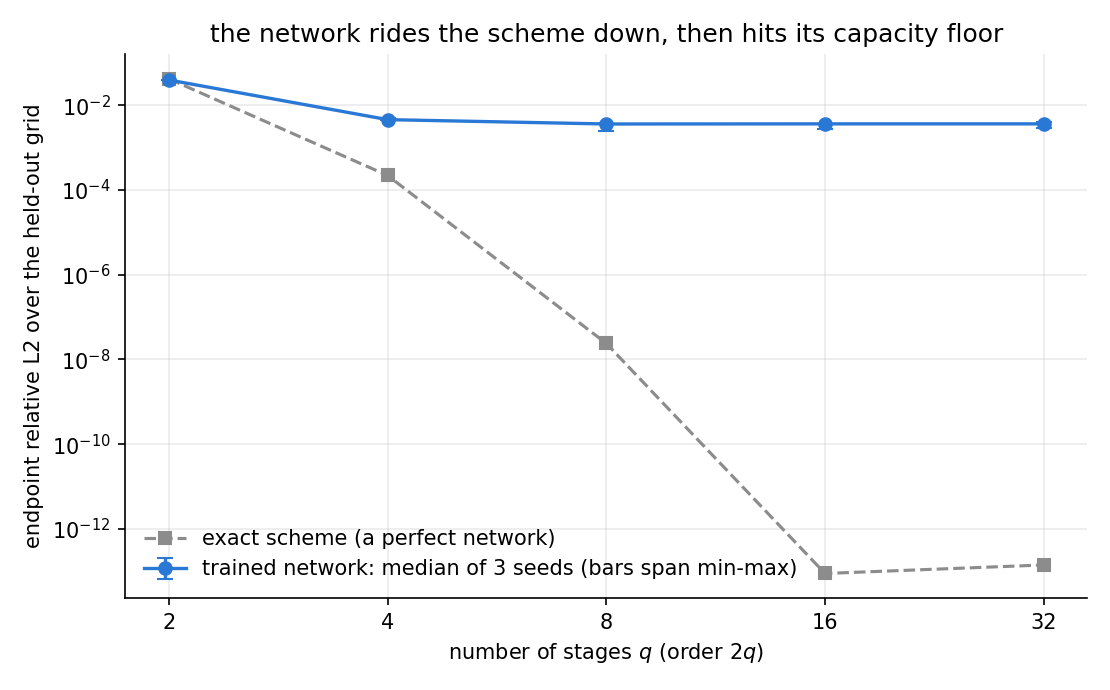
\includegraphics[width=0.72\linewidth]{fig_capacity_floor.png}
  \caption{Endpoint relative $L_2$ error versus number of stages: the
  trained network (median of three seeds, min--max whiskers) rides the
  scheme's error down and then flattens onto its floor, while the exactly
  solved scheme (grey) continues to machine precision.}
  \label{fig:floor}
\end{figure}

Training gives no trouble: all fifteen runs converge to
losses of $7\times10^{-6}$ to $2.6\times10^{-5}$ with no collapse and no
divergence, and, unlike every failed run of
Sections~\ref{sec:cont-results} and~\ref{sec:causal}, the loss is an
honest proxy for the error: a squared-residual loss of $10^{-5}$ resolves
outputs to roughly its square root, $3$--$5\times10^{-3}$, which is where
the held-out error lands.

Table~\ref{tab:floor} and Figure~\ref{fig:floor} give the central result
of this section. At $q = 2$ the trained network sits
\emph{on} the exactly solved scheme's own error: the map is
scheme-limited, and even a perfect fit would be that wrong. From $q = 4$
the curves part: the scheme drops ten orders of magnitude to roundoff
while the network stays flat at $3.6$--$4.6\times10^{-3}$ (within a factor
$1.27$ for all $q \ge 4$, all seeds agreeing). The remaining error belongs
to the network rather than the scheme, so more stages cannot help; the
lever is the network itself, and Section~\ref{sec:disc-size} shows that
the binding constraint there is the optimisation rather than capacity. The
stages are learned as accurately as the endpoint at every $q$ (asking for
66 outputs at $q = 32$ instead of 18 at $q = 8$ degrades nothing), the
largest errors sit at the corners of the training region where the
dynamics are fastest, and the three seeds agree on this pattern (observed
in the saved per-state error maps; not shown). The floor is a property of
the method rather than an initialisation accident. All later
discrete-time studies fix $q = 8$: from $q = 4$ the network sets the
error, and at $q = 8$ the scheme's own error is five orders of magnitude
below the network's, so nothing about the network is masked by the
scheme.

\subsection{The capped measure, and the error as a distribution}
\label{sec:disc-rho}

\begin{table}[tbp]
  \centering
  \caption{The capped measure of Eq.~\eqref{eq:rho} on the 441-state grid
  (median over three seeds of the per-run values; exactly one capped
  point per run, the state whose true image is the origin). The mean
  column is pinned at that point's fixed $1/441 \approx 2.3\times10^{-3}$
  contribution from $q \ge 4$ and resolves nothing below it; this is the
  reporting rule of Section~\ref{sec:metrics} in action.}
  \label{tab:rho}
  \small
  \begin{tabular}{ccc}
    \toprule
    $q$ & median $\rho$ & mean $\rho$ (dominated by the capped point) \\
    \midrule
    2  & $7.2\times10^{-5}$ & $3.5\times10^{-3}$ \\
    4  & $1.0\times10^{-5}$ & $2.3\times10^{-3}$ \\
    8  & $6.5\times10^{-6}$ & $2.3\times10^{-3}$ \\
    16 & $6.0\times10^{-6}$ & $2.3\times10^{-3}$ \\
    32 & $5.1\times10^{-6}$ & $2.3\times10^{-3}$ \\
    \bottomrule
  \end{tabular}
\end{table}

In the capped measure (Table~\ref{tab:rho}) the median column tracks the
floor: $\sqrt{6.5\times10^{-6}} \approx 2.5\times10^{-3}$ at $q=8$,
consistent with the relative $L_2$ floor as it must be. On the test
set (108 held-out starting states, each chained 50 steps, six periods, by
the three $q=8$ networks of Section~\ref{sec:disc-results}, 16{,}200
(state, time, seed) values) not a
single value reaches the cap: the pooled median is $1.8\times10^{-4}$ at
two periods and $1.7\times10^{-3}$ at six, the worst single value anywhere
in the set is $6.6\times10^{-2}$, and the smallest true state modulus
encountered is $0.063$, so the measure is defined everywhere with no
exclusions (Figure~\ref{fig:testset}).

\begin{figure}[tbp]
  \centering
  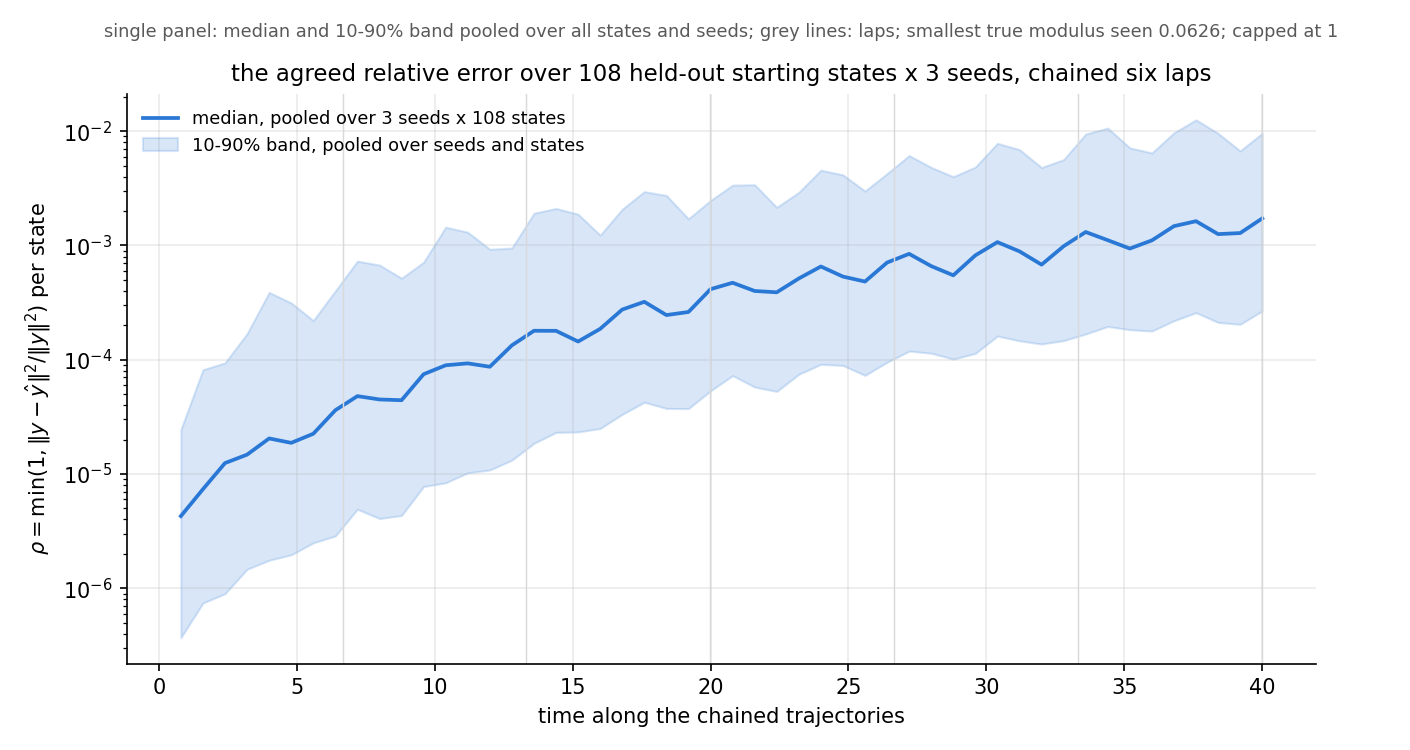
\includegraphics[width=\linewidth]{fig_test_set.png}
  \caption{The error as a distribution rather than a single trajectory:
  the capped measure $\rho$ over the pooled test set (three seeds
  $\times$ 108 held-out starting states, each chained 50 steps) against
  time; median and 10--90\% band. The drift is slow and repeats with the
  oscillator's period; nothing is excluded.}
  \label{fig:testset}
\end{figure}

\subsection{Network size, the seed, and selection}
\label{sec:disc-size}

The continuous-time route's size study has a discrete-time twin, with a
different question to test: is the $3.6\times10^{-3}$ floor a capacity
limit? The design crosses depth $\{2,\dots,10\}$ with width
$\{16, 32, 64, 128, 256\}$ (45 architectures) at fixed $q = 8$, three
seeds each, 135 runs, everything else frozen; each network is scored
one-step on the 441-state grid and chained fifty steps (six periods) over
the 108-start test set. Seven architectures spanning the usable band and
its edges (2$\times$64, 4$\times$32, 4$\times$50, 4$\times$64,
4$\times$128, 4$\times$256, 8$\times$128) were then trained at ten seeds
each. For honesty the 108 test starts are split: 50 of the
Latin-hypercube starts form a validation set used only to rank trained
networks, and the remaining 58 (the 8 named reference starts plus 50
Latin-hypercube starts) are held out and used only to report the chosen
network, so the reported numbers cannot be flattered by the selection. A
network's six-period error ranks almost identically on the two halves
(rank correlation $+0.989$), which is what makes selection meaningful.
Four findings.

\emph{The floor does not move.} The best of 45 architectures
(3 layers $\times$ 128 units) reaches $2.5\times10^{-3}$, a factor 1.5
below the 4$\times$50 configuration's $3.6\times10^{-3}$, and still five
orders of magnitude above the exact scheme
(Figure~\ref{fig:size-map-discrete}).
Depth beyond about 5 hurts sharply (depths 2--5: median $4.6\times10^{-3}$;
depths 7--10: median $1.8\times10^{-2}$); width stops helping beyond
64--128; the worst corner (10 $\times$ 16) sits at $1.3\times10^{-1}$.

\emph{The binding constraint is the optimiser, not capacity.} Across the
135-run grid, the Spearman rank correlation between converged training
loss and held-out one-step error (the correlation of the two quantities'
rank orderings, so that $+1$ means the run with the $k$-th smallest loss
also has the $k$-th smallest error for every $k$) is $+0.974$:
architectures that fail also fail to train. There is no capacity-rich,
badly-generalising regime, and every run used its full budget of six
restarts. The floor of Section~\ref{sec:disc-results} is an optimisation
floor. (The same training loss ranks six-period chained error at only
$+0.35$; the distinction between the two errors matters and is the
subject of the next two findings.)

\emph{Long horizons are decided by the seed, not the architecture.} I
measure error growth under chaining as the ratio of a network's median
six-period $\rho$ to its median one-period $\rho$. This ratio varies
${\sim}13\times$ between seeds of a single architecture and
${\sim}300\times$ across the grid; the 4$\times$50 configuration's
ten-seed median ratio is 28, with only one seed in ten staying within a
factor 3 of its one-period error. For no architecture does the error
reliably stop growing. Comparing each candidate's ten-seed six-period
errors against the 4$\times$50 configuration with Mann--Whitney tests,
Bonferroni-corrected across the candidates (threshold $p < 0.0083$), the
width-64 architectures' absolute improvement is significant
($p \approx 0.006$) while the three-seed grid's apparent best,
4$\times$128, is not ($p = 0.12$); and even the significant
architectures' seed spreads span decades
(Figure~\ref{fig:seed-replication}).

\emph{But growth is a measurable, transferable property of the trained
network.} A validation chain to the target horizon predicts held-out
six-period error at Spearman $+0.98$; the training loss and the one-step
error predict it at only $+0.35$, and a one-period chain at $+0.67$.
Hence the selection protocol:
\begin{enumerate}
  \item train about ten seeds of the chosen architecture;
  \item chain each on the validation starts to the target horizon; and
  \item keep the seed with the smallest validation error.
\end{enumerate}
Selection beats the median seed by 3--96$\times$ per architecture.
Ranked by the six-period validation chain and reported on the held-out
half, the selected seeds of the seven candidates reach six-period $\rho$
between $2.0\times10^{-6}$ (4$\times$32) and $4.8\times10^{-5}$
(8$\times$128); the 4$\times$32 candidate gave the smallest held-out
six-period error. A far-horizon check then separated the front-runners:
chained to thirty periods ($t = 200$) from twenty fresh starts, the
4$\times$32 choice moved from $3.1\times10^{-6}$ to $3.4\times10^{-6}$
(a factor 1.1), while the 4$\times$64, 4$\times$128 and 4$\times$50
choices grew by factors 11.3, 8.7 and 24
(Figure~\ref{fig:selection}). On this basis the 4$\times$32 seed-9
network ($3{,}858$ parameters) is the network reported throughout the
rest of the paper. The far-horizon check also carries a caveat: a
six-period validation window does not guarantee thirty periods for every
candidate, so the protocol's window should match the horizon the map
will be used at.

\begin{figure}[tbp]
  \centering
  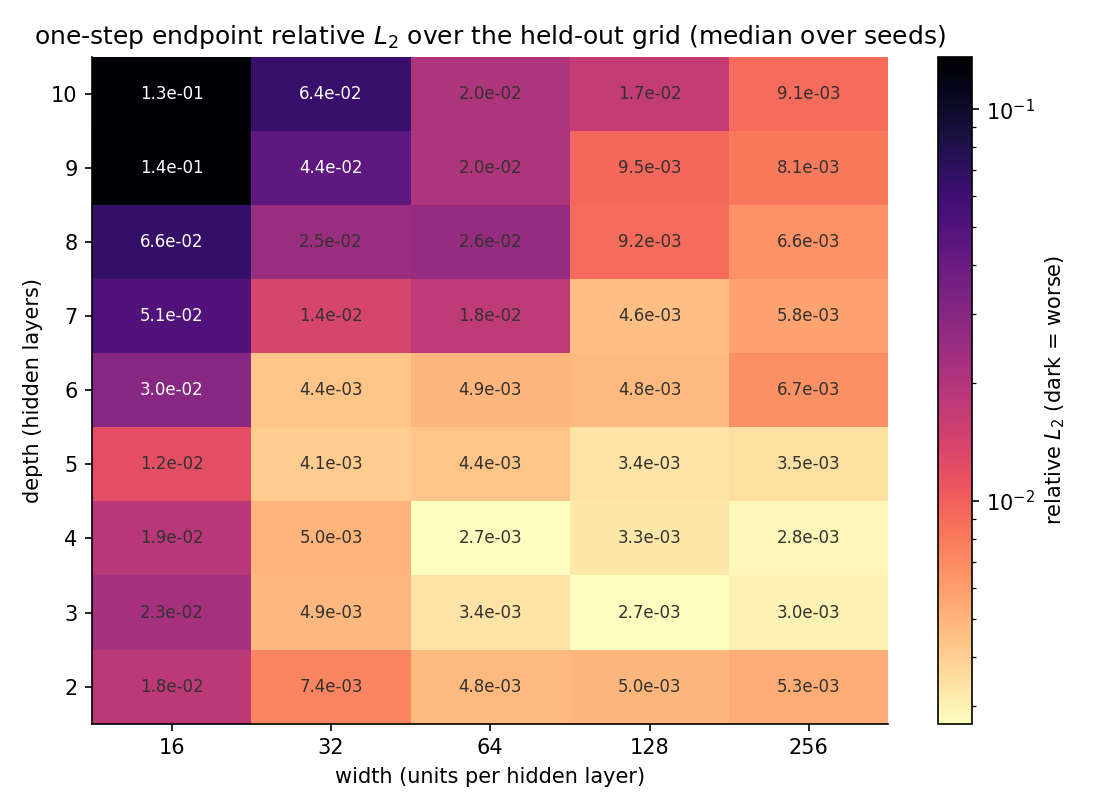
\includegraphics[width=\linewidth]{fig_size_map_discrete.png}
  \caption{One-step error over the architecture grid at fixed $q=8$: no
  entry approaches the exactly solved scheme; depth harms, width stops
  helping beyond 64--128. The floor is not a capacity floor.}
  \label{fig:size-map-discrete}
\end{figure}

\begin{figure}[tbp]
  \centering
  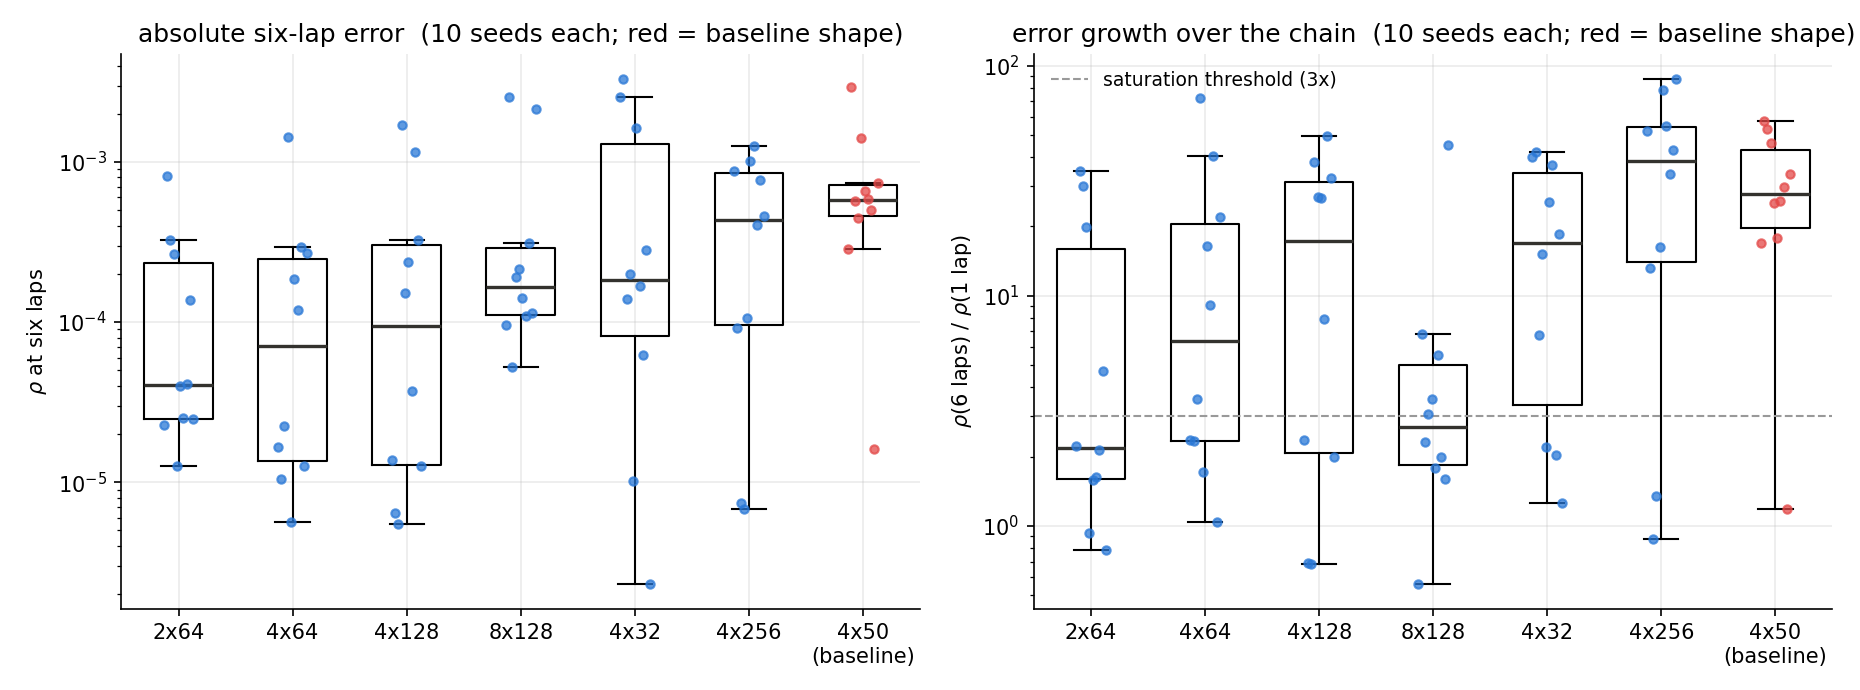
\includegraphics[width=\linewidth]{fig_seed_replication.png}
  \caption{Ten seeds for seven architectures, six-period chained error:
  the seed-to-seed spread within one architecture rivals the whole
  grid's spread. The seed, not the shape, decides the horizon.}
  \label{fig:seed-replication}
\end{figure}

\begin{figure}[tbp]
  \centering
  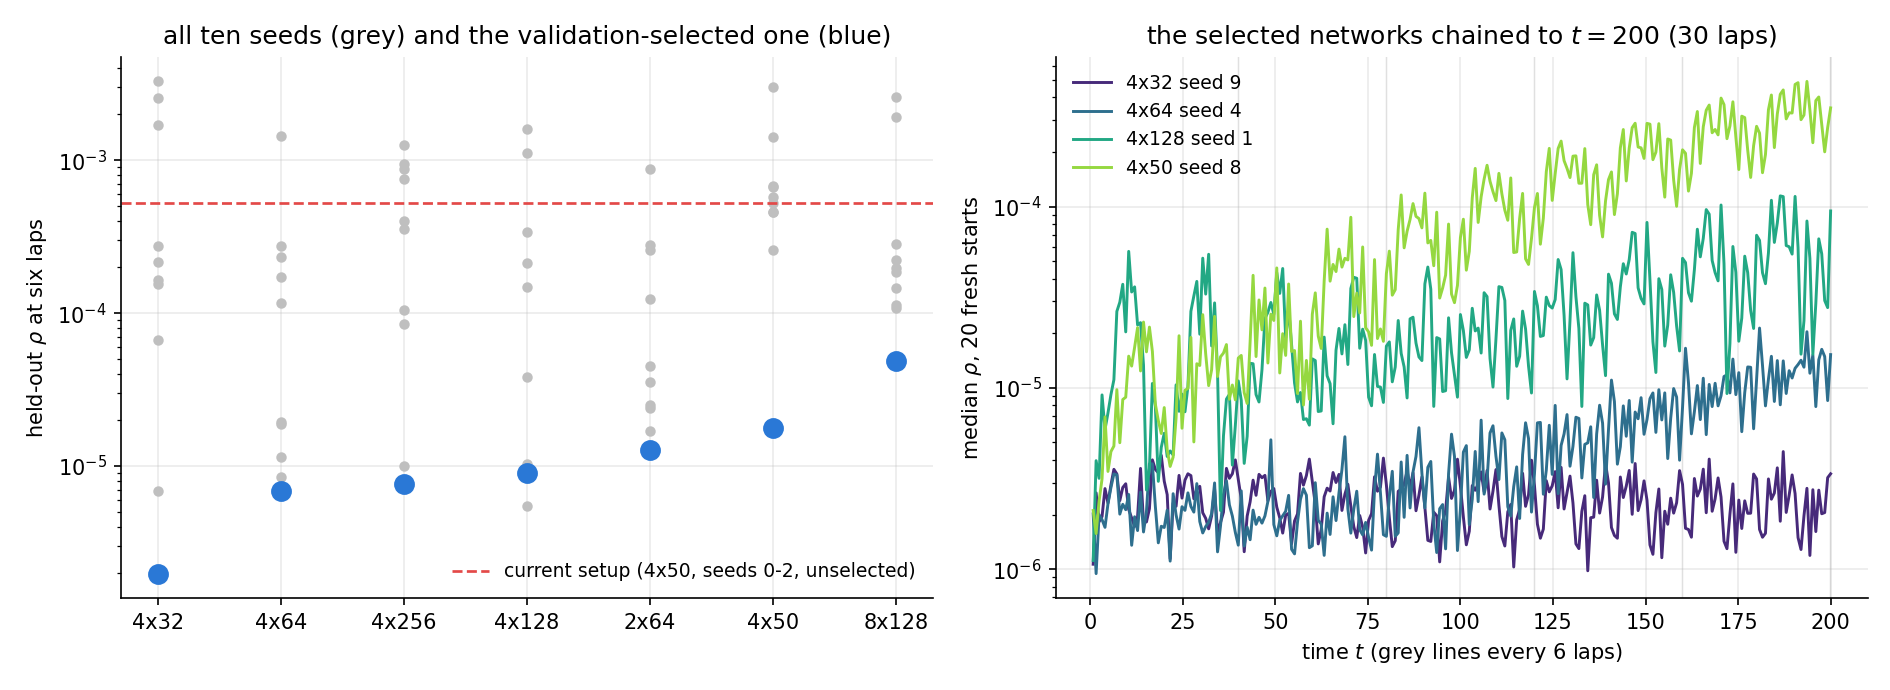
\includegraphics[width=\linewidth]{fig_selection.png}
  \caption{The selection payoff and the far-horizon check:
  validation-selected networks against their unselected siblings, and the
  selected 4 $\times$ 32 network holding $\rho \approx 3\times10^{-6}$
  flat to thirty periods on fresh starts.}
  \label{fig:selection}
\end{figure}

\subsection{Whole trajectories: chaining versus one large step}
\label{sec:disc-routes}

How should the one-step technique deliver the actual goal, a starting
state in and a whole trajectory out? The source work's discrete-time
formulation can be read in two ways. Route A chains the trained one-step
map: feed the endpoint back in, no retraining, reaching a horizon $T$ in
steps of $\Delta t = 0.8$ (50 chained steps at $T = 40$, six periods).
Route B generalises the source work's demonstration on the Allen--Cahn
equation, which it solves with a single large implicit step: here, one
network learns one large step whose stage states are the trajectory
readout. Route B's feasibility was checked first with the exact solver:
at a full period in one step ($\Delta t = 6.66$) the stage equations
stop being reliably solvable even at $q = 64$ (solver success 90 of 100
states). A-stability is a linear property; what actually binds is
nonlinear solvability. The largest feasible large step is half a period
($\Delta t = 3.2$ at $q = 64$), and Route B was trained there (three
seeds). The classical comparison of Section~\ref{sec:cont-results} sits
on the other side of the same trade: at $\Delta t = 0.8$ the explicit
order-6 method is not finite past $t = 8.8$, while the implicit scheme
the network imitates takes that step at $2.4\times10^{-8}$ one-step
error, and the trained map at $3.6\times10^{-3}$.

\begin{table}[tbp]
  \centering
  \caption{Whole trajectories over the continuous-time sweep's horizons:
  relative $L_2$ error over all chained step times up to $T$, per start,
  with the median pooled over the three seeds and the 108 test starts
  (single network for the selected column). The last column lists, for
  scale, the plain variant's dedicated single-start fits of
  Section~\ref{sec:cont-results}; the causally weighted variant reaches
  $7.6\times10^{-5}$ at $T=7$ and $2.1\times10^{-4}$ at $T=14$ for its
  single training start (Section~\ref{sec:causal}) and exceeds unity at
  $T \ge 27$.}
  \label{tab:routes}
  \small
  \begin{tabular}{cccl}
    \toprule
    $T$ & Route A, 4$\times$50 seeds & Route A, selected 4$\times$32 & continuous-time, plain \\
    \midrule
    3  & $2.6\times10^{-3}$ & $1.6\times10^{-3}$ & $3.8\times10^{-5}$ (dedicated fit, one start) \\
    7  & $4.8\times10^{-3}$ & $2.1\times10^{-3}$ & $6.6\times10^{-4}$ (dedicated fit, one start) \\
    14 & $9.0\times10^{-3}$ & $2.1\times10^{-3}$ & $0.79$ \\
    27 & $1.8\times10^{-2}$ & $2.1\times10^{-3}$ & $0.90$ \\
    40 & $2.6\times10^{-2}$ & $2.0\times10^{-3}$ & $0.94$ \\
    \bottomrule
  \end{tabular}
\end{table}

Table~\ref{tab:routes} and Figures~\ref{fig:headtohead}
and~\ref{fig:route-a-selected} give the result. The 4$\times$50 seeds
compound gently, from $2.6\times10^{-3}$ at half a period to
$2.6\times10^{-2}$ at six; the selected network's column is flat at
$1.6$--$2.1\times10^{-3}$ from half a period to six periods (the $T=40$
value over the $T=3$ value is a factor 1.3). The map has stopped
compounding, and at six periods it is twelve times better than the best
unselected seed. Against Route B at the matched horizon ($T = 3.2$,
i.e.\ four chained steps of $0.8$ against one large step of $3.2$):
Route A selected $2.1\times10^{-3}$ versus Route B $2.0\times10^{-2}$,
so chaining beats the one-step-per-horizon mode by a factor 10 (already
6.6$\times$ with the 4$\times$50 seeds, $3.0\times10^{-3}$ versus
$2.0\times10^{-2}$; Figure~\ref{fig:route-b-vs-a}). Chained trajectories
may briefly leave the training rectangle (4 starts of 108, per seed);
all return within one step. The loop's attraction corrects the radial
direction on its own, and the surviving error is mostly slow drift in
where along the loop the state sits at a given time, visible as the
settled period: $6.6573$ measured against the true $6.663287$
($-0.09\%$).

Two caveats apply to the comparison with the continuous-time column.
The continuous-time error is evaluated on the dense reference grid while
the chained error is evaluated at the step times, and each
continuous-time network was trained for its specific horizon and single
starting state while a single discrete map serves all horizons and all
108 starts: the comparison is between formulations rather than matched
estimators. The other direction is also visible in
Table~\ref{tab:routes}: below one period the dedicated continuous-time
fits are more accurate (up to forty times, for the plain fits at
$T = 3$), and the causally weighted fit at $T=14$ beats the chained
map's pooled median for its one trained start. The chained map's
advantage is that it serves every start in the region at every horizon;
from four periods onward no continuous-time variant produces a usable
trajectory while the chained map's pooled median stays at
$2\times10^{-3}$.

\begin{figure}[tbp]
  \centering
  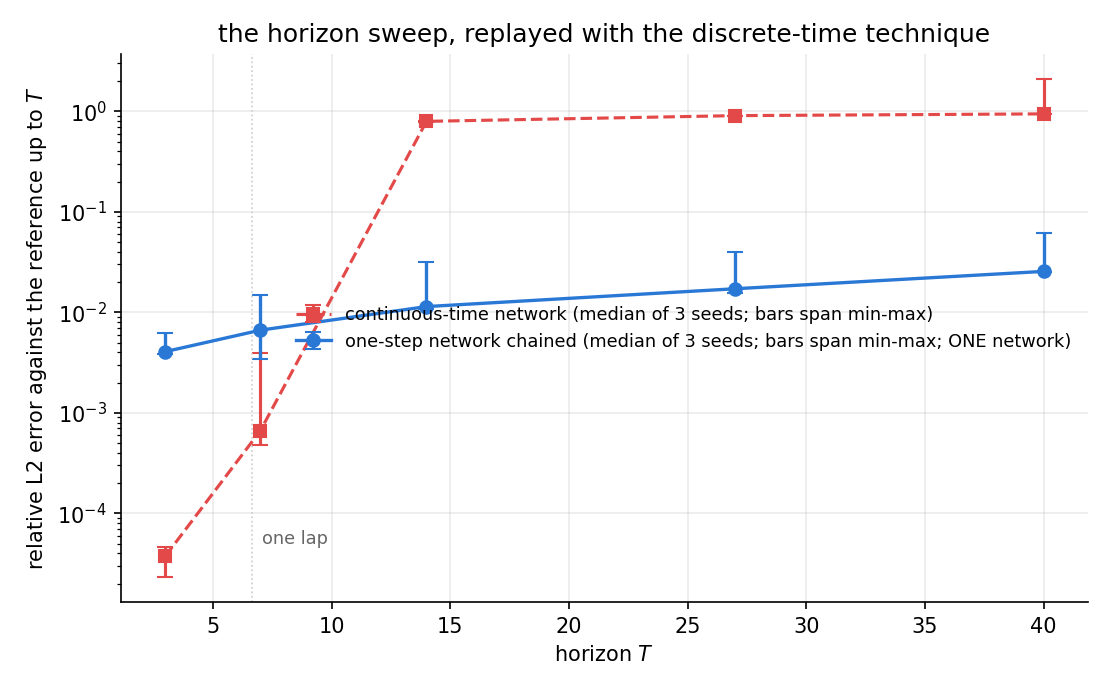
\includegraphics[width=0.8\linewidth]{fig_head_to_head.png}
  \caption{Both formulations on one axis, at the continuous-time sweep's
  horizons; the continuous-time points show the plain variant (the
  causally weighted variant reaches $2.1\times10^{-4}$ at two periods
  for its single training start and exceeds unity from four). The
  chained map's pooled median rises gently where the continuous-time
  fits fail at order one; below one period the dedicated fits are the
  more accurate.}
  \label{fig:headtohead}
\end{figure}

\begin{figure}[tbp]
  \centering
  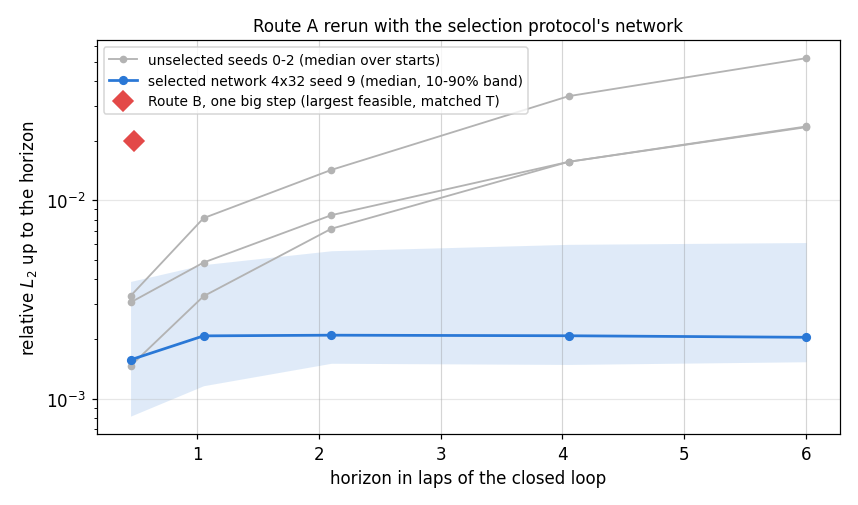
\includegraphics[width=\linewidth]{fig_route_a_selected.png}
  \caption{The selected network against the unselected 4$\times$50
  seeds, chained over the test set: a compounding
  $2.3$--$5.2\times10^{-2}$ six-period map becomes a flat
  $2.0\times10^{-3}$ one.}
  \label{fig:route-a-selected}
\end{figure}

\begin{figure}[tbp]
  \centering
  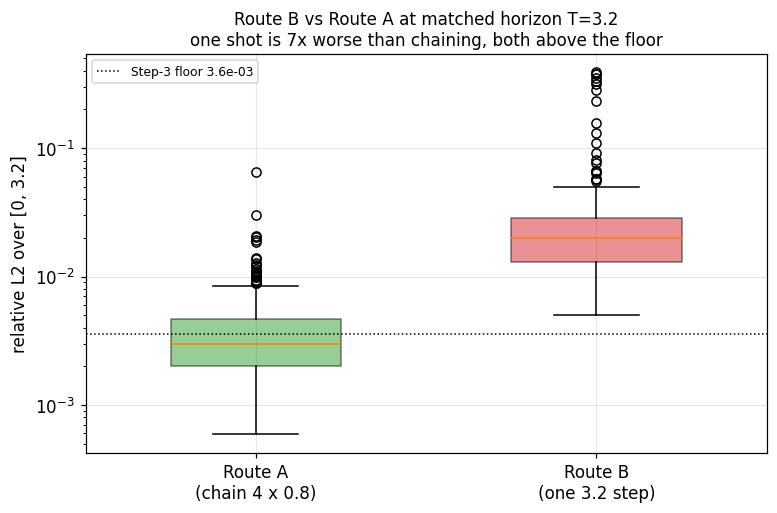
\includegraphics[width=\linewidth]{fig_route_b_vs_a.png}
  \caption{Route B (one large half-period step, stage states as the
  trajectory readout) against Route A at the matched horizon: the
  one-step-per-horizon mode is an order of magnitude worse, and a
  full-period step is not even reliably solvable.}
  \label{fig:route-b-vs-a}
\end{figure}

\subsection{Training from labels instead: a matched comparison}
\label{sec:baseline}

If perfect solution data were available, would it beat the physics? The
test is a matched pair: identical network, identical seeded initial
weights, identical optimiser and budget; the only differences are the
loss, \emph{physics} (the reconstructions of Eq.~\eqref{eq:recon}, as
everywhere above) versus \emph{data} (mean squared error to the true
stage states and endpoint, computed by the reference integrator), and
the training-set size $n \in \{50, 125, 250, 500, 1000, 2000\}$, three
seeds each, 36 runs.

\begin{table}[tbp]
  \centering
  \caption{Physics-trained versus data-trained (perfect labels) at matched
  everything else: endpoint relative $L_2$ on the 441-state grid, medians
  over three seeds, against training-set size $n$. The last column is the
  reference-integrator work needed to label the data variant's training
  set, at 799 steps per state.}
  \label{tab:baseline}
  \small
  \begin{tabular}{cccc}
    \toprule
    $n$ & physics (median) & data (median) & integrator steps for labels \\
    \midrule
    50   & $9.2\times10^{-3}$ & $9.8\times10^{-3}$ & $39{,}950$ \\
    125  & $6.3\times10^{-3}$ & $3.0\times10^{-3}$ & $99{,}875$ \\
    250  & $4.1\times10^{-3}$ & $1.8\times10^{-3}$ & $199{,}750$ \\
    500  & $3.4\times10^{-3}$ & $1.6\times10^{-3}$ & $399{,}500$ \\
    1000 & $3.4\times10^{-3}$ & $1.7\times10^{-3}$ & $799{,}000$ \\
    2000 & $3.6\times10^{-3}$ & $1.6\times10^{-3}$ & $1{,}598{,}000$ \\
    \bottomrule
  \end{tabular}
\end{table}

Both variants flatten from $n \approx 500$: the physics medians read
$3.4$, $3.4$, $3.6\times10^{-3}$ at $n = 500$, $1000$, $2000$ and the
data medians $1.6$, $1.7$, $1.6\times10^{-3}$, a stable factor of about
2.1 apart, with the physics variant ahead only at $n = 50$
(Table~\ref{tab:baseline} and Figure~\ref{fig:data-baseline}; the
$n = 2000$ physics entry is the run of Section~\ref{sec:disc-results}).
The last column is the important one, and its accounting is explicit:
the labels for one training state are the eight true stage states plus
the true endpoint, produced by running the reference integrator of
Section~\ref{sec:problem} across the step at its working step size
$10^{-3}$, halting exactly at each stage time; that is 799 integrator
steps of $10^{-3}$ to traverse the step of $0.8$ once, so the column
reads $799\,n$.\footnote{Outside synthetic tests, labels of this quality
are not available; even these carry the full reference method inside
them.} The physics variant's reference cost is exactly zero at every
$n$. The physics loss therefore gives up a factor of about 2.1 in
accuracy relative to perfect labels and in exchange needs no reference
data at all. On the source of the remaining gap: the data loss's
minimiser is the true stage states, while the physics loss's minimiser
is the scheme's stage states; at $q=8$ these differ by about
$2.4\times10^{-8}$ on this grid (Table~\ref{tab:floor}), five orders
below either variant's error, so at this accuracy the gap between the
variants is not an information gap, and the findings are consistent with
the two losses differing in the path the optimiser takes rather than in
what they specify.

\begin{figure}[tbp]
  \centering
  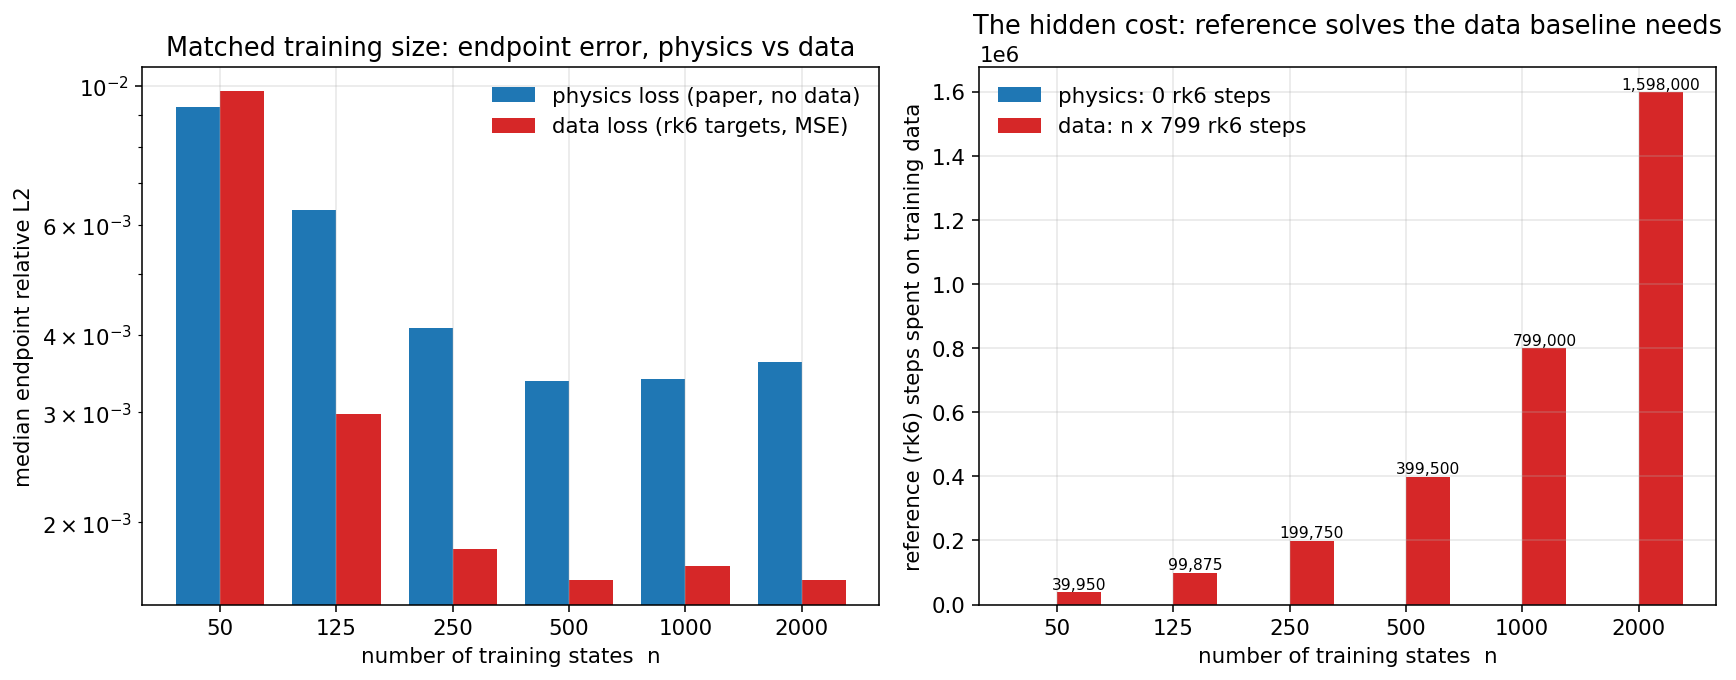
\includegraphics[width=\linewidth]{fig_data_baseline.png}
  \caption{Accuracy against training-set size for the matched pair (left)
  and the reference-integrator work behind the data variant's labels
  (right): the physics variant's reference-data bill is zero everywhere.}
  \label{fig:data-baseline}
\end{figure}

% ===========================================================================
\section{Discussion}
\label{sec:discussion}

\paragraph{Relation to the source work.}
Where the regimes overlap, the reproduction agrees: on sub-period
horizons, the same regime as the source work's continuous-time solution
demonstrations (the Burgers equation on $t \in [0,1]$; the Schr\"odinger
equation on $t \in [0, \pi/2]$), the
transcription meets or betters the reported accuracy of a few $10^{-4}$ to
$2\times10^{-3}$. Where the source work stops, the measurements sharpen it
in three ways. First, it frames the continuous-time formulation's principal
limitation as the \emph{cost} of collocation in higher dimensions. On this
problem the collocation budget is trivial and fully paid
(Section~\ref{sec:collocation}), was then varied 64-fold and re-placed
with no effect (Sections~\ref{sec:density}
and~\ref{sec:placement}), and the formulation fails anyway, through
optimisation collapse onto zero-residual spurious solutions with a
converged loss. This runs directly against its stated expectation, and
across 733 runs rather than the 15 of the reproduction alone, so cost is
not the binding limitation on long horizons even in one dimension.
Second, on the discrete-time side
the source work attributes its Allen--Cahn error to network capacity, and
its appendix tables already contain a visible error floor (its $q$-sweep
at $\Delta t = 0.8$ flattens at $7\times10^{-4}$--$1.2\times10^{-3}$ from
$q = 16$ to $q = 500$); what it lacks is the exactly solved scheme on the
same states and metric, which is what turns a plateau in a table into an
attribution (scheme-limited at $q = 2$, network-limited from $q = 4$).
The 135-run architecture sweep then goes one step further than the source
work's capacity attribution: the $+0.974$ rank correlation between
training loss and one-step error makes the floor an optimisation floor,
which no network size fixes. Third, its stage-count prescription (choose
$q$ so that the theoretical $\mathcal{O}(\Delta t^{2q})$ truncation
reaches machine precision, giving $q \approx 81$ at $\Delta t = 0.8$) is
far past the point of usefulness once the optimisation binds: at $q = 8$
the scheme already sits five orders of magnitude below the floor.
Finally, the source work's suggestion that a single large implicit step
can resolve the entire solution does not transfer unconditionally: on
this system the nonlinear stage equations stop being reliably solvable
near a full-period step, a solvability limit, distinct from stability,
that the source work does not discuss, and at the largest feasible step
chaining beats the single-step mode by a factor 10
(Section~\ref{sec:disc-routes}).

\paragraph{Relation to the causal-weighting literature.}
Causal weighting behaves as its authors report~\cite{wang2024causal}: it
addresses the pathology it targets, the simultaneous fitting of all
times, at a training cost that grows quickly with the domain, and their
own guidance that causal weighting complements rather than replaces
time-marching~\cite{wang2023expert} is precisely what
Sections~\ref{sec:causal} and~\ref{sec:disc-routes} measure from the two
sides. A fixed look-back window (weighting each point only by the residual
of the preceding period) was considered and rejected without an
experiment: a fit that jumps once and then follows a different genuine
solution of the equation has zero residual inside every window older than
the jump, so windowing re-admits exactly the silent failures of
Section~\ref{sec:cont-results}. The whole-history
integral in Eq.~\eqref{eq:causal} is what keeps the not-yet-reached part
of the domain out of the fit, and the same integral is what makes the
weight condition harder to meet as the horizon grows. The density study
adds one fact to this literature: the weight condition itself has a
density floor (about 20 points per unit time here) below which it is met
on wrong solutions (Section~\ref{sec:density}). The failure
modes measured here sit within the broader literature on PINN optimisation
pathologies~\cite{wang2021gradient,krishnapriyan2021}, with more instrumentation per failure than is usual.

\paragraph{Relation to the fixed-point literature.}
The failure study places this chapter's measurements inside the account of Rohrhofer et al.~\cite{rohrhofer2023}, who showed that fixed points of the dynamical system are global minima of the physics loss, and extends it: the fixed point is the cheapest member of a family of exactly zero-residual splices, any trajectory of the flow can be spliced in, and the family's price under resampling is of order $1/T$, which the parked runs of Section~\ref{sec:axes} reproduce to within a few percent from four to fifteen periods. The regulariser of Babic et al.~\cite{babic2025} does exactly what its construction says and no more: it prices sitting still at an unstable fixed point, cures the horizons where the origin was the only member in play, and at four periods and beyond hands the optimiser the next member of the family, an off-loop trajectory joined in the first unsampled gap, in every variant including their published protocol. Their van der Pol horizons stopped at two periods, which is why they did not see this. Pseudo-time stepping~\cite{wang2026pseudo} is the only method tested whose mechanism prices the whole family, and it is the only one that works past two periods; its authors tested partial differential equations and did not consider fixed points or phase, so the van der Pol result is a new instance of their theorem rather than a reproduction. What none of the three papers gives, and this chapter adds, is the converged failure anatomy: which member of the family each objective settles on, at what loss, and the fact that the loss keeps falling on the wrong member while the error does not move.

\paragraph{The recurring observation.}
The equation alone admits many solutions, and any stretch of the domain the
loss cannot see is eventually exploited by the optimiser: late times in the
plain formulation, the intervals between collocation points in the causally
weighted one. Each modification closed one such opening and exposed the
next, at increasing cost. The resource axes are all measured and none changes the outcome at four periods; what does change it is the objective: pricing the whole family of spliced solutions, as pseudo-time stepping does, moves the wall from two periods to six, and nothing tested moves it past ten.
Two corollaries deserve emphasis. Phase-plane
agreement is necessary but never sufficient: an orbit can lie exactly on
the limit cycle and be order-one wrong in time
(Figure~\ref{fig:extended-phase}). And in every failure the training loss
was small: the verdict must always come from the error against a trusted
reference at points the training never saw, and never from the loss. The
discrete-time formulation removes the disease rather than treating it:
every output is tied to a known state through the algebra of the step, so
a spurious solution has nowhere to live. Consistently with that, it is
also the only formulation here whose loss predicts its one-step error, all
the way to a rank correlation of $+0.974$ across 135 architectures.

% ===========================================================================
\section{Future work}
\label{sec:future}

Six studies follow naturally from these measurements; I list them in the
order I would run them.

\begin{itemize}
  \item \textbf{A sweep of the step size.} Every discrete-time result in
  this paper is at the single step $\Delta t = 0.8$ taken from the
  source work. The trade between step size, stage count, solvability and
  network error is unmeasured, and the chained map's error budget per
  period depends directly on it; this is the axis I would test first.
  \item \textbf{Attribution of the optimisation floor.} The 135-run sweep
  rules out capacity; what it does not yet separate is optimiser dynamics
  from the loss landscape: whether a different optimiser class, training
  schedule, or curriculum over the training region moves the
  $3.6\times10^{-3}$ floor at fixed architecture.
  \item \textbf{The late parks of pseudo-time stepping.} Its failures at six to fifteen periods ride the loop for four to eight periods and then park. What sets that position, the adaptive $\tau$ schedule, the anchor's fading influence or the $1/T$ price finally undercutting the truth, is unmeasured; the per-run telemetry of Section~\ref{sec:arms} is the instrument, and a fixed-$\tau$ arm and a starting-state sweep are the first two runs.
  \item \textbf{An extension check of the regulariser protocol.} Its three successes at four periods and density 80 are budget-limited; extending them, and the causal $\varepsilon \propto 1/T$ variant suggested by the weight condition's hardening with horizon, closes the two loose ends of the continuous route.
  \item \textbf{Inverse problems.} The source work's data-driven discovery
  setting, recovering the damping parameter $\mu$ from noisy
  observations, has a natural discrete-time variant that reuses exactly
  the trained reconstructions with $\mu$ as a free parameter.
  \item \textbf{Learned quadrature.} A variant in which the network
  predicts the step's weights rather than its states, for which the
  fine-grained single-step reference built for this study provides the
  supervision.
\end{itemize}

% ===========================================================================
\section{Conclusion}
\label{sec:conclusion}

On a fully controlled nonlinear oscillator with a reference solution
trusted to $10^{-13}$, the continuous-time PINN formulation is excellent
below one period of the limit cycle and fails structurally beyond it,
collapsing onto zero-residual spurious solutions while its training loss
converges. In these measurements, no resource changed that outcome: ample
collocation, a four-fold optimisation budget, 25 network architectures at
600 runs, a 64-fold density range, and targeted re-placement of the collocation points. A supervised control showed the same networks fitting four periods from data, so the fault lies in the objective: it is exactly satisfied by a family of spliced trajectories of which the fixed point is the cheapest, at a price that falls like $1/T$ and is measured to do so. Every published fix works at two periods; the fixed-point regulariser, in every variant, converges onto the next member of the family past them, and only pseudo-time stepping, which prices the whole family, carries the formulation to six periods, with its own wall short of ten. The strongest loss-level modification short of that moves the
failure out by one period at a cost that grows faster than linearly, and
what orders the outcomes is the starting state: success at two periods
occurred in 19 of 150 causally weighted runs at the 1\% threshold, and at
four periods in none of 300. The
discrete-time formulation, generalised into a reusable one-step map over
starting states, inherited none of this in these tests. Its supervision
is anchored to a known state by the algebra of an implicit Runge--Kutta
step, its training loss predicts its one-step error, and its accuracy is
cleanly attributable: scheme-limited at two stages, floored at
$3.6\times10^{-3}$ from four by the optimisation rather than by
capacity. Its long-horizon quality, decided by the training seed, is
measurable on a validation chain and controlled by a simple selection
protocol. The selected network, chained without retraining, carried 108
held-out starting states through six periods at $2.0\times10^{-3}$
relative error, held flat to thirty periods on fresh starts, and beat
the single-large-step reading of the source work by a factor 10 at the
largest step the nonlinear algebra allowed; a matched data-trained twin
shows the physics loss costing a factor of about 2.1 in accuracy against
perfect labels, with no reference data needed in exchange. For
initial-value problems on long horizons, these findings favour
formulations that re-anchor the physics on known states step by step;
and on this problem the binding failure of the continuous-time
formulation was not the cost of enforcing the equation, but the optimiser's freedom to satisfy it on the wrong solution, a freedom this chapter has now measured, priced, and, up to six periods, removed.

% ---------------------------------------------------------------------------
\section*{Data availability}

All training scripts, saved results, and the notebooks that generate every
figure and number in this paper are available at
\url{https://github.com/GeorgeWilliam1999/Van_Der_Pole}. All experiments
are seeded and reproduce deterministically; the reference solution and its
verification are included.

% \section*{Acknowledgements}
% TODO before submission.

\bibliographystyle{unsrtnat}
\bibliography{references}

\end{document}
